
%preamble
\documentclass[11pt, mathserif, aspectratio=169]{beamer}
\usetheme{Boadilla}
\usefonttheme{serif}

\addtobeamertemplate{frametitle}{\vspace*{0.2in}\hspace*{0.5in}}{\vspace*{0.3cm}}
\setbeamersize{text margin left=.7in,text margin right=.7in}
\setbeamercolor{author in head/foot}{fg=black!50!white, bg=white}
\setbeamercolor{title in head/foot}{fg=black!50!white, bg=white}
\setbeamerfont{footline}{size=\scriptsize,shape=\itshape}
\makeatother
\setbeamertemplate{footline}
{
  \leavevmode%
  \hbox{%
  \begin{beamercolorbox}[wd=.3\paperwidth,ht=2.5ex,dp=1.5ex,center]{author in head/foot}%
    \usebeamerfont{author in head/foot}\insertshortauthor
  \end{beamercolorbox}%
  \begin{beamercolorbox}[wd=.7\paperwidth,ht=2.5ex,dp=1.5ex,center]{title in head/foot}%
    \usebeamerfont{title in head/foot}\insertshorttitle\hspace*{3em}
    \insertframenumber{} / \inserttotalframenumber\hspace*{1.5ex}
  \end{beamercolorbox}}%
  \vskip0pt%
}
\makeatletter
\setbeamertemplate{navigation symbols}{}

%% Method to add QR code onto every slide
%\addtobeamertemplate{footline}{%
%  \setlength\unitlength{1ex}%
%  \begin{picture}(0,0) 
%    % \put{} defines the position of the frame
%    \put(132,55){\makebox(0,0)[br]{
%    \includegraphics[scale=.045]{pics/QG2019-qr-code.png}
%    }}%
%  \end{picture}%
%}{}

\usepackage{amsmath, amsthm, graphicx, amssymb}
\usepackage{color}
\usepackage{colortbl}
\usepackage{setspace}
\usepackage{tabularx,booktabs,adjustbox}
\usepackage{pifont}
\usepackage{tikz}
\usetikzlibrary{calc,fit,arrows,decorations.pathmorphing,decorations.footprints,backgrounds,fit,positioning}
\usetikzlibrary{shapes.symbols}
\usepackage[style=authoryear]{biblatex}
%\usepackage{cellspace}
%\setlength\cellspacetoplimit{1.5ex}
%\setlength\cellspacebottomlimit{1.5ex}

% Define a colour-blind-friendly palette.
%
% From:
% http://wiki.stdout.org/rcookbook/Graphs/Colors%20%28ggplot2%29/
\definecolor{Cblack}{rgb}{0,0,0}
\definecolor{Corange}{rgb}{0.9,0.6,0}
\definecolor{Cskyblue}{rgb}{0.35,0.7,0.9}
\definecolor{Cbluegreen}{rgb}{0,0.6,0.5}
\definecolor{Cyellow}{rgb}{0.95,0.9,0.25}
\definecolor{Cblue}{rgb}{0,0.45,0.7}
\definecolor{Cvermillion}{rgb}{0.8,0.4,0}
\definecolor{Cpurple}{rgb}{0.8,0.6,0.7}

% Define other colours.
\definecolor{grey}{gray}{0.8}

% Convenient colouring commands.
\newcommand{\red}[1]{\textcolor{red}{#1}}
\newcommand{\green}[1]{\textcolor{green}{#1}}
\newcommand{\blue}[1]{\textcolor{blue}{#1}}
\newcommand{\grey}[1]{\textcolor{grey}{#1}}
\newcommand{\white}[1]{\textcolor{white}{#1}}
\newcommand{\Cblack}[1]{\textcolor{Cblack}{#1}}
\newcommand{\Corange}[1]{\textcolor{Corange}{#1}}
\newcommand{\Cskyblue}[1]{\textcolor{Cskyblue}{#1}}
\newcommand{\Cbluegreen}[1]{\textcolor{Cbluegreen}{#1}}
\newcommand{\Cyellow}[1]{\textcolor{Cyellow}{#1}}
\newcommand{\Cblue}[1]{\textcolor{Cblue}{#1}}
\newcommand{\Cvermillion}[1]{\textcolor{Cvermillion}{#1}}
\newcommand{\Cpurple}[1]{\textcolor{Cpurple}{#1}}
\newcommand{\magenta}[1]{\textcolor{magenta}{#1}}
\newcommand{\gray}[1]{\textcolor{gray}{#1}}


%commands
\newcommand{\lt}{\left(}
\newcommand{\ls}{\left[}
\newcommand{\rt}{\right)}
\newcommand{\rs}{\right]}
\newcommand{\ts}{\thinspace}
\newcommand{\emp}[0]{\it}
\newcommand{\R}{\mathbb{R}}
\newcommand{\N}{\mathbb{N}}
\newcommand{\Var}{\mathrm{Var}}
\newcommand{\ds}{\displaystyle}
\newcommand{\be}{\beta}
\newcommand{\al}{\alpha}
\newcommand{\ga}{\gamma}
\newcommand{\p}{\mathbf{P}}
\newcommand{\E}{\mathbf{E}}
\newcommand{\Vari}{\mathrm{Var}}
\newcommand{\Cov}{\mathrm{Cov}}
\newcommand{\Corr}{\mathrm{Corr}}
\newcommand{\as}{\overset{a.s.}{\longrightarrow}}
\newcommand{\distn}{\overset{d}{\longrightarrow}}
% Checks and crosses
\newcommand{\crossmark}{\ding{55}}

% Rotating column headings in tables
\newcolumntype{R}[2]{%
    >{\adjustbox{angle=#1,lap=\width-(#2)}\bgroup}%
    l%
    <{\egroup}%
}
\newcommand*\rot{\multicolumn{1}{R{30}{1em}}}% no optional argument here, please!
% https://tex.stackexchange.com/questions/32683/rotated-column-titles-in-tabular

\AtBeginSection[]{
  \begin{frame}
  \vfill
  \centering
  \begin{beamercolorbox}[sep=8pt,center,shadow=true,rounded=true]{title}
    \usebeamerfont{title}\insertsectionhead\par%
  \end{beamercolorbox}
  \vfill
  \end{frame}
}

% environments
\newenvironment{wideitemize}{\itemize\addtolength{\itemsep}{10pt}}{\enditemize}


% packages
\usepackage{booktabs, hyperref}

% title
\titlegraphic{
\includegraphics[scale=.5]{pics/unimelb-logo.jpg}}
\title{Efficient simulation of introgression,\\ admixture and local ancestry}
\author{Georgia Tsambos}
\institute{{\normalsize University of Melbourne, Australia}}
\date{Quantitative Genomics, 10 June 2019}
% information

% tikz colour settings
\tikzset{pop1/.style={blue!40},pop2/.style={red!40}}


% start of document

\begin{document}

\maketitle

\begin{frame}
\frametitle{Talk outline}

\begin{enumerate}
\itemsep7mm
\item[1. ] Introduction to admixture and local ancestry
\item[2. ] Tree sequences
\item[3. ] Simulating local ancestry with tree sequences: existing methods
\item[4. ] Simulating local ancestry with tree sequences: new method
\end{enumerate}
\end{frame}

\section{Intro to admixture and local ancestry}


\begin{frame}
\frametitle{What is admixture?}
%\begin{minipage}[t][2cm][t]{\textwidth}
%\begin{center}
%
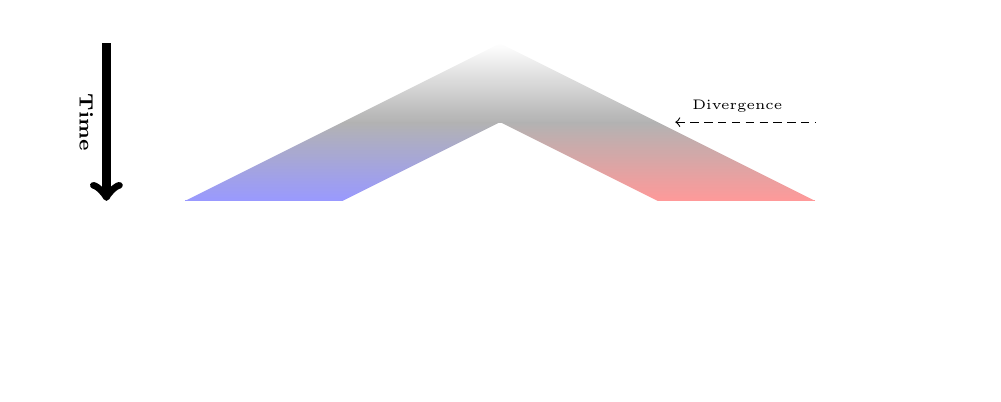
\begin{tikzpicture}[xscale=.4,yscale=.2,auto]

\clip (-15, 1) rectangle (15,-21);

% Nodes
\node (mcra) at (0,0) {};
\node (admix-event) at (0,10) {};
\node (pop1) at (-10,0) {};
\node (pop2) at (10,0) {};
\node (popsize) at (5,0) {};
\node (admix-gens) at (0,10) {};
\node (split-time) at (0,5) {};
\node (adm-popsize) at ($0.5*(popsize)$) {};

% The Population tree
\node[inner sep=0] (transition1) at ($-1*(popsize) - (split-time)$) {};
\node[inner sep=0] (transition2) at ($(popsize) - (split-time)$) {};
\shade[top color=white,bottom color=black!30] (mcra.center) -- (transition1.center) -- (transition2.center) -- cycle;
\shade[top color=black!30,bottom color=blue!40] (transition1.center) -- ++(transition1.center) -- ++(popsize.center) -- ++($-1*(transition1)$) -- cycle;
\shade[top color=black!30,bottom color=red!40] (transition2.center) -- ++(transition2.center) -- ++($-1*(popsize.center)$) -- ++($-1*(transition2)$) -- cycle;
%\shade[top color=blue!40,bottom color=blue!80] ($2*(transition1)$) -- ++($-1*(admix-gens)$) -- ++(popsize.center) -- ++(admix-gens.center) -- cycle;
%\shade[top color=red!40,bottom color=red!80] ($2*(transition2)$) -- ++($-1*(admix-gens)$) -- ++($-1*(popsize.center)$) -- ++(admix-gens.center) -- cycle;

%% The admixed population
%\shade[top color=purple!40,bottom color=purple!80] ($(mcra) - 2*(split-time) - 0.5*(adm-popsize)$) -- ++(adm-popsize.center) -- ++($-1*(admix-gens)$) -- ++($-1*(adm-popsize)$) -- cycle;
%
%% The admixture arrows
%\draw[->,>=stealth,blue,semithick,shorten <=1mm,shorten >=1mm] ($-1*(split-time) + (transition1)$) -- +($0.75*(popsize)$);
%\draw[->,>=stealth,red,semithick,shorten <=1mm,shorten >=1mm] ($-1*(split-time) + (transition2)$) -- +($-0.75*(popsize)$);

% The time arrows
\draw[->,line width=3pt] ($(mcra) - 2.5*(popsize)$) -- node[below,rotate=270] {\bf\scriptsize Time} ++($-2*(split-time)$) ;;

% Time labels
\draw[<-,densely dashed,shorten <=2mm] (transition2) -- node[above] {\tiny Divergence}  ++(5,0);
%\draw[<-,densely dashed,shorten <=2mm] ($2*(transition2)$) -- node[above] {\tiny Admixture}   ++(5,0);
%\draw[<-,densely dashed,shorten <=2mm] ($2*(transition2) - (admix-gens)$) -- node[above] {\tiny Present day}   ++(5,0);

% Fill in annoying white lines
\draw[black!30] (transition1) -- (transition2);
\draw[blue!40] ($2*(transition1)$) -- +(5,0);
\draw[red!40] ($2*(transition2)$) -- +(-5,0);


\end{tikzpicture}  


%\end{center}
%\end{minipage}

\begin{wideitemize}
%\item In the context of my work: {\it a group of people.}
%\item {\it Recombination, mutation, selection and drift} act over time to differentiate  populations that have split from each other.
%\item Analysing these differences are the basis for methods that infer the ancestry of DNA from people with mixed, or unknown backgrounds...
    \item An organism has \magenta{ancestry} with a given population if they have inherited some genetic material from ancestors who belonged to that population. 
    \item Any organism with $>1$ ancestry is \magenta{admixed}.
    \item \magenta{Introgression} is admixture between different species.
\end{wideitemize}

\end{frame}

%\begin{frame}
%\frametitle{What is admixture?}
%\begin{minipage}[t][2cm][t]{\textwidth}
%\begin{center}
%
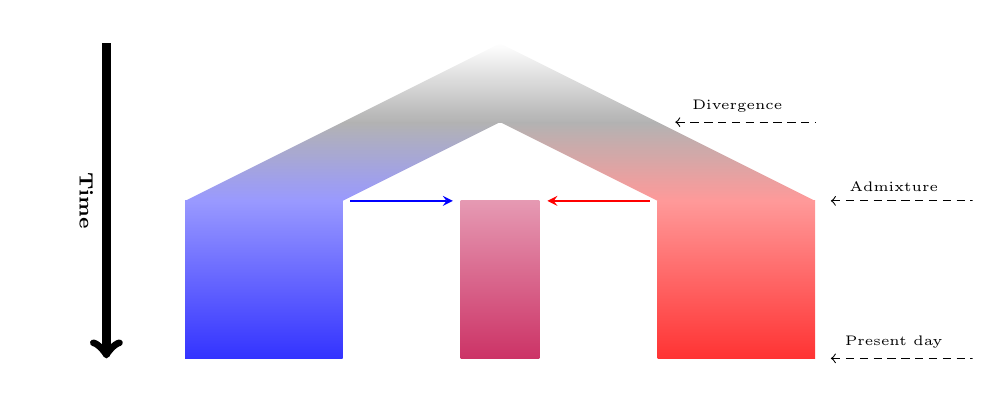
\begin{tikzpicture}[xscale=.4,yscale=.2,auto]

\clip (-15, 1) rectangle (15,-21);

% Nodes
\node (mcra) at (0,0) {};
\node (admix-event) at (0,10) {};
\node (pop1) at (-10,0) {};
\node (pop2) at (10,0) {};
\node (popsize) at (5,0) {};
\node (admix-gens) at (0,10) {};
\node (split-time) at (0,5) {};
\node (adm-popsize) at ($0.5*(popsize)$) {};

% The Population tree
\node[inner sep=0] (transition1) at ($-1*(popsize) - (split-time)$) {};
\node[inner sep=0] (transition2) at ($(popsize) - (split-time)$) {};
\shade[top color=white,bottom color=black!30] (mcra.center) -- (transition1.center) -- (transition2.center) -- cycle;
\shade[top color=black!30,bottom color=blue!40] (transition1.center) -- ++(transition1.center) -- ++(popsize.center) -- ++($-1*(transition1)$) -- cycle;
\shade[top color=black!30,bottom color=red!40] (transition2.center) -- ++(transition2.center) -- ++($-1*(popsize.center)$) -- ++($-1*(transition2)$) -- cycle;
\shade[top color=blue!40,bottom color=blue!80] ($2*(transition1)$) -- ++($-1*(admix-gens)$) -- ++(popsize.center) -- ++(admix-gens.center) -- cycle;
\shade[top color=red!40,bottom color=red!80] ($2*(transition2)$) -- ++($-1*(admix-gens)$) -- ++($-1*(popsize.center)$) -- ++(admix-gens.center) -- cycle;

% The admixed population
\shade[top color=purple!40,bottom color=purple!80] ($(mcra) - 2*(split-time) - 0.5*(adm-popsize)$) -- ++(adm-popsize.center) -- ++($-1*(admix-gens)$) -- ++($-1*(adm-popsize)$) -- cycle;

% The admixture arrows
\draw[->,>=stealth,blue,semithick,shorten <=1mm,shorten >=1mm] ($-1*(split-time) + (transition1)$) -- +($0.75*(popsize)$);
\draw[->,>=stealth,red,semithick,shorten <=1mm,shorten >=1mm] ($-1*(split-time) + (transition2)$) -- +($-0.75*(popsize)$);

% The time arrows
\draw[->,line width=3pt] ($(mcra) - 2.5*(popsize)$) -- node[below,rotate=270] {\bf\scriptsize Time} ++($-4*(split-time)$) ;;

% Time labels
\draw[<-,densely dashed,shorten <=2mm] (transition2) -- node[above] {\tiny Divergence}  ++(5,0);
\draw[<-,densely dashed,shorten <=2mm] ($2*(transition2)$) -- node[above] {\tiny Admixture}   ++(5,0);
\draw[<-,densely dashed,shorten <=2mm] ($2*(transition2) - (admix-gens)$) -- node[above] {\tiny Present day}   ++(5,0);

% Fill in annoying white lines
\draw[black!30] (transition1) -- (transition2);
\draw[blue!40] ($2*(transition1)$) -- +(5,0);
\draw[red!40] ($2*(transition2)$) -- +(-5,0);


\end{tikzpicture}  


%\end{center}
%\end{minipage}
%
%%{\small
%%\begin{wideitemize}
%%    \item A person has {\bf ancestry} with a given population if they have inherited some genetic material from ancestors who belonged to that population. 
%%    \item Any person with $>1$ ancestry is {\bf admixed}.
%%    \item Migrations that bring together historically distinct populations are {\bf admixture~events}.
%%\end{wideitemize}
%%}
%\end{frame}

\begin{frame}
%\frametitle{What is admixture?}
\begin{center}


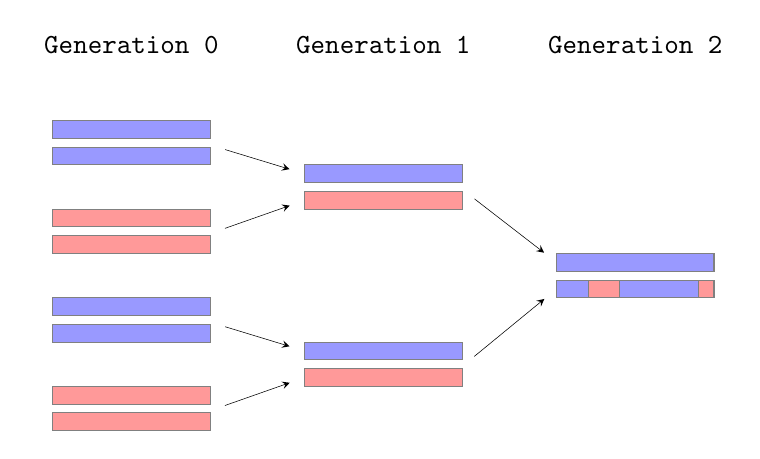
\begin{tikzpicture}[yscale=0.15, xscale=0.2]

\tikzset{
pop1/.style={fill=blue!40,draw=black!50},
pop2/.style={fill=red!40,draw=black!50},
inherit/.style={->,>=stealth,ultra thin,shorten <=2mm,shorten >=2mm,very thin},
recomb/.style={thick,draw=black!70}
}

% Nodes
\node (hapx) at (1,0) {};
\node (hapy) at (0,1.5) {};
\node (hapxy) at ($10*(hapx) + (hapy)$) {};

\node (gen1) at (0,0) {};
\node (gen2) at ($8*(hapx) + 0*(hapx)$) {};
\node (gen3) at ($8*(hapx) + 8*(hapx)$) {};

\node (ind1gen3) at ($(gen3) + (0,0)$) {};
\node (indsep) at ($5*(hapy)$) {};

\node (ind1gen2) at ($(gen2) + 1*(indsep)$) {};
\node (ind2gen2) at ($(gen2) - 1*(indsep)$) {};

\node (ind1gen1) at ($(gen1) + 1.5*(indsep)$) {};
\node (ind2gen1) at ($(gen1) + 0.5*(indsep)$) {};
\node (ind3gen1) at ($(gen1) - 0.5*(indsep)$) {};
\node (ind4gen1) at ($(gen1) - 1.5*(indsep)$) {};

\node (chr1) at ($0.25*(hapy)$)  {};
\node (chr2) at ($-1.25*(hapy)$) {};


% Haplotypes

\filldraw[pop1] ($(gen1) + (ind1gen1) + (chr1)$) rectangle +(hapxy);
\filldraw[pop1] ($(gen1) + (ind1gen1) + (chr2)$) rectangle +(hapxy);

\filldraw[pop2] ($(gen1) + (ind2gen1) + (chr1)$) rectangle +(hapxy);
\filldraw[pop2] ($(gen1) + (ind2gen1) + (chr2)$) rectangle +(hapxy);

\filldraw[pop1] ($(gen1) + (ind3gen1) + (chr1)$) rectangle +(hapxy);
\filldraw[pop1] ($(gen1) + (ind3gen1) + (chr2)$) rectangle +(hapxy);

\filldraw[pop2] ($(gen1) + (ind4gen1) + (chr1)$) rectangle +(hapxy);
\filldraw[pop2] ($(gen1) + (ind4gen1) + (chr2)$) rectangle +(hapxy);


\filldraw[pop1] ($(gen2) + (ind1gen2) + (chr1)$) rectangle +(hapxy);
\filldraw[pop2] ($(gen2) + (ind1gen2) + (chr2)$) rectangle +(hapxy);

\filldraw[pop1] ($(gen2) + (ind2gen2) + (chr1)$) rectangle +(hapxy);
\filldraw[pop2] ($(gen2) + (ind2gen2) + (chr2)$) rectangle +(hapxy);


\filldraw[pop1] ($(gen3) + (ind1gen3) + (chr1)$) rectangle +(hapxy);
\fill[pop1] ($(gen3) + (ind1gen3) + (chr2)$) rectangle +(hapxy);
\fill[pop2] ($(gen3) + (ind1gen3) + (chr2)+ 2*(hapx)$) rectangle ($(gen3) + (ind1gen3) + (chr2)+ (hapxy)$);
\fill[pop1] ($(gen3) + (ind1gen3) + (chr2)+ 4*(hapx)$) rectangle ($(gen3) + (ind1gen3) + (chr2)+ (hapxy)$);
\fill[pop2] ($(gen3) + (ind1gen3) + (chr2)+ 9*(hapx)$) rectangle ($(gen3) + (ind1gen3) + (chr2)+ (hapxy)$);
%\draw ($(gen3) + (ind1gen3) + (chr2)$) rectangle +(hapxy);


% Copying lines

\node (startline) at ($-1*(hapx) + 0.5*(hapy)$) {};
\node (chrdiff) at ($(chr1) - (chr2)$) {};

%\node (hapx) at (1,0) {};

%\draw[recomb] ($(gen1) + (ind1gen1) + (chr1) + (startline)$) -- ++($(hapx)$) --  ++($4*(hapx)$) --  ++($-1*(chrdiff)$) -- ++($2*(hapx)$) -- ++($(chrdiff)$) -- ++($4*(hapx)$) -- ++($1*(hapx)$);
%\draw[recomb] ($(gen1) + (ind2gen1) + (chr2) + (startline)$) -- ++($(hapx)$) -- ++($10*(hapx)$) --  ++($(hapx)$);
%\draw[recomb] ($(gen1) + (ind3gen1) + (chr1) + (startline)$) -- ++($(hapx)$) -- ++($10*(hapx)$) --  ++($(hapx)$);
%\draw[recomb] ($(gen1) + (ind4gen1) + (chr2) + (startline)$) -- ++($(hapx)$) --  ++($5*(hapx)$) --  ++($(chrdiff)$) -- ++($2*(hapx)$) -- ++($3*(hapx)$) -- ++($1*(hapx)$);
%
%\draw[recomb] ($(gen2) + (ind1gen2) + (chr1) + (startline)$) -- ++($(hapx)$) -- ++($10*(hapx)$) --  ++($(hapx)$);
%\draw[recomb] ($(gen2) + (ind2gen2) + (chr1) + (startline)$) -- ++($(hapx)$) --  ++($2*(hapx)$) --  ++($-1*(chrdiff)$) -- ++($2*(hapx)$) -- ++($(chrdiff)$) -- ++($3*(hapx)$) -- ++($2*(hapx)$) -- ++($-1*(chrdiff)$) -- ++($(hapx)$) -- ++($(hapx)$) ;


% Arrows
\draw[inherit] ($(gen1) + (ind1gen1) + (chr2) + 10*(hapx) + 0.75*(chrdiff)$) -- ($(gen2) + (ind1gen2) + (chr1) + 0.5*(hapy)$);
\draw[inherit] ($(gen1) + (ind2gen1) + (chr2) + 10*(hapx) + 0.75*(chrdiff)$) -- ($(gen2) + (ind1gen2) + (chr2) + 0.5*(hapy)$);
\draw[inherit] ($(gen1) + (ind3gen1) + (chr2) + 10*(hapx) + 0.75*(chrdiff)$) -- ($(gen2) + (ind2gen2) + (chr1) + 0.5*(hapy)$);
\draw[inherit] ($(gen1) + (ind4gen1) + (chr2) + 10*(hapx) + 0.75*(chrdiff)$) -- ($(gen2) + (ind2gen2) + (chr2) + 0.5*(hapy)$);

\draw[inherit] ($(gen2) + (ind1gen2) + (chr2) + 10*(hapx) + 0.75*(chrdiff)$) -- ($(gen3) + (ind1gen3) + (chr1) + 0.5*(hapy)$);
\draw[inherit] ($(gen2) + (ind2gen2) + (chr2) + 10*(hapx) + 0.75*(chrdiff)$) -- ($(gen3) + (ind1gen3) + (chr2) + 0.5*(hapy)$);


% Labels
\node (lab1) at ($(gen1) + 2.5*(indsep) + 0.5*(hapxy)$) {$\texttt{Generation 0}$};
\node (lab2) at ($2*(gen2) + 2.5*(indsep) + 0.5*(hapxy)$) {$\texttt{Generation 1}$};
\node (lab3) at ($4*(gen2) + 2.5*(indsep) + 0.5*(hapxy)$) {$\texttt{Generation 2}$};

\end{tikzpicture}

\end{center}
\end{frame}


\begin{frame}
\frametitle{Reporting ancestry}
\begin{center}

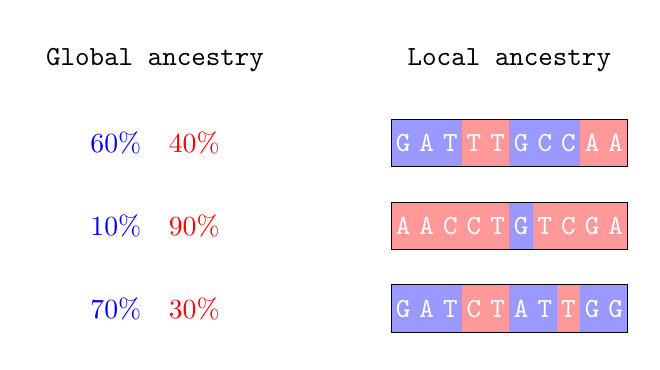
\begin{tikzpicture}[scale=0.3]

% Nodes
\node (glo) at (-12.5,0) {};
\node (loc) at (2.5,0)  {};

\node (rowheight) at (0,-3.5) {};
\node (row1) at ($(0,0) + (rowheight)$)   {};
\node (row2) at ($(0,0) + 2*(rowheight)$) {};
\node (row3) at ($(0,0) + 3*(rowheight)$) {};

\node (hapx) at (10,0) {};
\node (hapy) at (0,2)  {};
\node (hap)  at ($(hapx) + (hapy)$) {};


% Haplotype 1
\fill[pop1] ($(loc) + (row1)$) rectangle ($(loc) + (row1) + (hap)$) {};
\fill[pop2] ($(loc) + (row1) + 0.3*(hapx)$) rectangle ($(loc) + (row1) + (hap)$) {};
\fill[pop1] ($(loc) + (row1) + 0.5*(hapx)$) rectangle ($(loc) + (row1) + (hap)$) {};
\fill[pop2] ($(loc) + (row1) + 0.8*(hapx)$) rectangle ($(loc) + (row1) + (hap)$) {};
\draw ($(loc) + (row1)$) rectangle ($(loc) + (row1) + (hap)$) {};

% Haplotype 2
\fill[pop2] ($(loc) + (row2)$) rectangle ($(loc) + (row2) + (hap)$) {};
\fill[pop1] ($(loc) + (row2) + 0.5*(hapx)$) rectangle ($(loc) + (row2) + (hap)$) {};
\fill[pop2] ($(loc) + (row2) + 0.6*(hapx)$) rectangle ($(loc) + (row2) + (hap)$) {};
\draw ($(loc) + (row2)$) rectangle ($(loc) + (row2) + (hap)$) {};

% Haplotype 3
\fill[pop1] ($(loc) + (row3)$) rectangle ($(loc) + (row3) + (hap)$) {};
\fill[pop2] ($(loc) + (row3) + 0.3*(hapx)$) rectangle ($(loc) + (row3) + (hap)$) {};
\fill[pop1] ($(loc) + (row3) + 0.5*(hapx)$) rectangle ($(loc) + (row3) + (hap)$) {};
\fill[pop2] ($(loc) + (row3) + 0.7*(hapx)$) rectangle ($(loc) + (row3) + (hap)$) {};
\fill[pop1] ($(loc) + (row3) + 0.8*(hapx)$) rectangle ($(loc) + (row3) + (hap)$) {};
\draw ($(loc) + (row3)$) rectangle ($(loc) + (row3) + (hap)$) {};

% Global ancestry labels
\node (glo1) at ($(glo) + (row1) + 0.5*(hap)$)  {$\textcolor{blue}{60\%}\quad\textcolor{red}{40\%}$};
\node (glo2) at ($(glo) + (row2) + 0.5*(hap)$)  {$\textcolor{blue}{10\%}\quad\textcolor{red}{90\%}$};
\node (glo3) at ($(glo) + (row3) + 0.5*(hap)$)  {$\textcolor{blue}{70\%}\quad\textcolor{red}{30\%}$};

% Allele labels
\node (midpt) at ($0.05*(hapx) + 0.5*(hapy)$) {};

\node (hap1-0) at ($(loc) + (row1)$)  {};
\node (l) at ($(hap1-0) + (midpt)$) {$\textcolor{white}{\texttt{G}}$};
\node (l) at ($(hap1-0) + (midpt) + 0.1*(hapx)$) {$\textcolor{white}{\texttt{A}}$};
\node (l) at ($(hap1-0) + (midpt) + 0.2*(hapx)$) {$\textcolor{white}{\texttt{T}}$};
\node (l) at ($(hap1-0) + (midpt) + 0.3*(hapx)$) {$\textcolor{white}{\texttt{T}}$};
\node (l) at ($(hap1-0) + (midpt) + 0.4*(hapx)$) {$\textcolor{white}{\texttt{T}}$};
\node (l) at ($(hap1-0) + (midpt) + 0.5*(hapx)$) {$\textcolor{white}{\texttt{G}}$};
\node (l) at ($(hap1-0) + (midpt) + 0.6*(hapx)$) {$\textcolor{white}{\texttt{C}}$};
\node (l) at ($(hap1-0) + (midpt) + 0.7*(hapx)$) {$\textcolor{white}{\texttt{C}}$};
\node (l) at ($(hap1-0) + (midpt) + 0.8*(hapx)$) {$\textcolor{white}{\texttt{A}}$};
\node (l) at ($(hap1-0) + (midpt) + 0.9*(hapx)$) {$\textcolor{white}{\texttt{A}}$};

\node (hap2-0) at ($(loc) + (row2)$)  {};
\node (l) at ($(hap2-0) + (midpt)$) {$\textcolor{white}{\texttt{A}}$};
\node (l) at ($(hap2-0) + (midpt) + 0.1*(hapx)$) {$\textcolor{white}{\texttt{A}}$};
\node (l) at ($(hap2-0) + (midpt) + 0.2*(hapx)$) {$\textcolor{white}{\texttt{C}}$};
\node (l) at ($(hap2-0) + (midpt) + 0.3*(hapx)$) {$\textcolor{white}{\texttt{C}}$};
\node (l) at ($(hap2-0) + (midpt) + 0.4*(hapx)$) {$\textcolor{white}{\texttt{T}}$};
\node (l) at ($(hap2-0) + (midpt) + 0.5*(hapx)$) {$\textcolor{white}{\texttt{G}}$};
\node (l) at ($(hap2-0) + (midpt) + 0.6*(hapx)$) {$\textcolor{white}{\texttt{T}}$};
\node (l) at ($(hap2-0) + (midpt) + 0.7*(hapx)$) {$\textcolor{white}{\texttt{C}}$};
\node (l) at ($(hap2-0) + (midpt) + 0.8*(hapx)$) {$\textcolor{white}{\texttt{G}}$};
\node (l) at ($(hap2-0) + (midpt) + 0.9*(hapx)$) {$\textcolor{white}{\texttt{A}}$};

\node (hap3-0) at ($(loc) + (row3)$)  {};
\node (l) at ($(hap3-0) + (midpt)$) {$\textcolor{white}{\texttt{G}}$};
\node (l) at ($(hap3-0) + (midpt) + 0.1*(hapx)$) {$\textcolor{white}{\texttt{A}}$};
\node (l) at ($(hap3-0) + (midpt) + 0.2*(hapx)$) {$\textcolor{white}{\texttt{T}}$};
\node (l) at ($(hap3-0) + (midpt) + 0.3*(hapx)$) {$\textcolor{white}{\texttt{C}}$};
\node (l) at ($(hap3-0) + (midpt) + 0.4*(hapx)$) {$\textcolor{white}{\texttt{T}}$};
\node (l) at ($(hap3-0) + (midpt) + 0.5*(hapx)$) {$\textcolor{white}{\texttt{A}}$};
\node (l) at ($(hap3-0) + (midpt) + 0.6*(hapx)$) {$\textcolor{white}{\texttt{T}}$};
\node (l) at ($(hap3-0) + (midpt) + 0.7*(hapx)$) {$\textcolor{white}{\texttt{T}}$};
\node (l) at ($(hap3-0) + (midpt) + 0.8*(hapx)$) {$\textcolor{white}{\texttt{G}}$};
\node (l) at ($(hap3-0) + (midpt) + 0.9*(hapx)$) {$\textcolor{white}{\texttt{G}}$};

% Column labels
\node (hapmidpt) at ($0.5*(hapx) + 0.5*(hapy)$) {};
\node (lab1) at ($(glo) + (hapmidpt)$) {$\texttt{Global ancestry}$};
\node (lab1) at ($(loc) + (hapmidpt)$) {$\texttt{Local ancestry}$};

\end{tikzpicture}

\end{center}
My PhD work is about \magenta{simulating} and inferring local ancestry.\\[2mm]

%Understanding local ancestry is important in studies of demography and history, medicine and genetic pipelines.
\end{frame}

\begin{frame}
\frametitle{Being able to simulate genetic ancestry is useful!}
\begin{wideitemize}
\item {\bf Benchmarking and evaluating method performance\\}
To assess the accuracy of methods that infer ancestry, we need test datasets in which we know the true local ancestry.
\item {\bf Model training\\}
Some methods for ancestry inference are trained on simulated data.
\item {\bf Exploration\\}
Simulations allow us to explore the influence of various historical scenarios on observed patterns of genetic variation and inheritance.
\end{wideitemize}
\end{frame}

%\begin{frame}
%\frametitle{Why is understanding admixture and ancestry important?}
%
%\begin{wideitemize}
%\item {\bf Demography and history\\} Inference about the dates and composition of historical migrations and admixture events. 
%\item {\bf Medicine\\} GWAS and risk prediction studies, admixture mapping studies.
%\item {\bf Genetic pipelines\\} Phasing and imputation.
%\end{wideitemize}
%
%\end{frame}


\section{Tree sequences: the data format}

\begin{frame}
\frametitle{Context: genetic data is BIG and REPETITIVE}
 \begin{center}
{\tt
%\ldots GTAACGCGATAAGAGATTAGCCCAAAAACACAGACATGGAAATAGCGTA\ldots \\
%\ldots GTAACGCGATAAGAGATTAGCCCAAAAACACAGACATGGAAATAGCGTA\ldots \\
\ldots GTAACGCGATAAGAGATTAGCCCAAAAACACAGACATGGAAATAGCGTA\ldots \\
\ldots GTAACGCGATAAGAGATTAGCCCAAAAACACAGACATGGAAATAGCGTA\ldots \\
\ldots GTAACGCGATAAGATATTAGCCCAAAAACACAGACATGGAAATAGCGTA\ldots \\
\ldots GTAACGCGATAAGATATTAGCCCAAAAACACAGACATGGAAATAGCGTA\ldots \\
\ldots GTAACGCGATAAGATATTAGCCCAAAAACACAGACATGGAAATAGCGTA\ldots \\
\ldots GTAACGCGATAAGATATTAGCCCAAAAACACAGACATGGTAATAGCGTA\ldots \\
%\ldots GTAACGCGATAAGATATTAGCCCAAAAACACAGACATGGTAATAGCGTA\ldots \\
%\ldots GTAACGCGATAAGATATTAGCCCAAAAACACAGACATGGTAATAGCGTA\ldots \\
\ldots GTAACGCGATAAGATATTAGCCCAAAAACACAGACATGGTAATAGCGTA\ldots \\[3mm]
}
\gray{\footnotesize $\leftarrow 5\times 10^7$ bases for small human chromosome $\rightarrow$}
\end{center}
Repeated haplotypes are often just a consequence of shared history.\\[3mm]
\magenta{\bf Q. Can we use this history to represent DNA sequences more compactly?}
\end{frame}

%\begin{frame}
%\frametitle{Context - genetic data is BIG and REPETITIVE}
%\begin{center}
%{\tt
%%\ldots GTAACGCGATAAGA\Cvermillion{G}ATTAGCCCAAAAACACAGACATGG\Cvermillion{A}AATAGCGTA\ldots \\
%%\ldots GTAACGCGATAAGA\Cvermillion{G}ATTAGCCCAAAAACACAGACATGG\Cvermillion{A}AATAGCGTA\ldots \\
%\ldots GTAACGCGATAAGA\Cvermillion{G}ATTAGCCCAAAAACACAGACATGG\Cvermillion{A}AATAGCGTA\ldots \\
%\ldots GTAACGCGATAAGA\Cvermillion{G}ATTAGCCCAAAAACACAGACATGG\Cvermillion{A}AATAGCGTA\ldots \\
%\ldots GTAACGCGATAAGA\Cskyblue{T}ATTAGCCCAAAAACACAGACATGG\Cvermillion{A}AATAGCGTA\ldots \\
%\ldots GTAACGCGATAAGA\Cskyblue{T}ATTAGCCCAAAAACACAGACATGG\Cvermillion{A}AATAGCGTA\ldots \\
%\ldots GTAACGCGATAAGA\Cskyblue{T}ATTAGCCCAAAAACACAGACATGG\Cvermillion{A}AATAGCGTA\ldots \\
%\ldots GTAACGCGATAAGA\Cskyblue{T}ATTAGCCCAAAAACACAGACATGG\Cskyblue{T}AATAGCGTA\ldots \\
%%\ldots GTAACGCGATAAGA\Cskyblue{T}ATTAGCCCAAAAACACAGACATGG\Cskyblue{T}AATAGCGTA\ldots \\
%%\ldots GTAACGCGATAAGA\Cskyblue{T}ATTAGCCCAAAAACACAGACATGG\Cskyblue{T}AATAGCGTA\ldots \\
%\ldots GTAACGCGATAAGA\Cskyblue{T}ATTAGCCCAAAAACACAGACATGG\Cskyblue{T}AATAGCGTA\ldots \\
%}
%\end{center}
%Shared haplotypes are often due to shared history.\\[3mm]
%
%\magenta{\bf Q. Can we use this history to store DNA more compactly?}
%\end{frame}


%\begin{frame}
%\frametitle{Tree sequences are the future!}
%\begin{wideitemize}
%\item Tree sequences contain rich information about the \magenta{history} of a sample, not just the genotypes.
%\item We can \magenta{simulate} this data structure using well-established software  (\texttt{msprime}, \texttt{SLiM}). (With some caveats...)
%\item We can \magenta{infer} this data structure with some success (\texttt{tsinfer}).
%%\item In Kelleher et al. (2018), a tree-sequence holding an estimated history of chrom 22 for $\approx$ 500K individuals in the UK Biobank is constructed. It is of comparable size to the corresponding BCF!  
%\end{wideitemize}
%\end{frame}

\begin{frame}
\frametitle{Trees show genealogy at a single locus}
\begin{minipage}{.48\textwidth}
\begin{center}

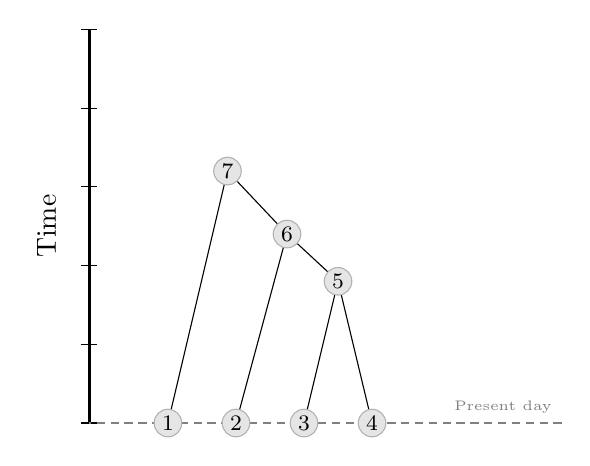
\begin{tikzpicture}[node distance=5mm and 5mm]

\tikzset{greynode/.style={font=\footnotesize,node distance=1cm and 1 cm,fill=black!10,draw=black!30,inner sep=0pt,minimum size=3.5mm,shape=circle},
mutations/.style={shape=starburst,fill=red!50!blue,inner sep=0.8pt,starburst points=11,starburst point height=.2cm}}

% Axis
\node (leftAx) at (-1,0) {};
\draw[very thick] (-1,0) -- +(0, 5);
\foreach \y in {0, 1, 2, 3, 4, 5} \draw ($(leftAx) + (-0.1, \y)$) -- ($(leftAx) + (0.1, \y)$); % tick marks
%\node[anchor=east] at ($(leftAx)$) {0}; \node[anchor=east] at ($(leftAx) + (0,5)$) {5};
\node[rotate=90,anchor=south] (leftLabel) at ($(leftAx) + (-0.3,2.5)$) {$\textrm{Time}$};

% Time arrow
\draw[densely dashed,color=gray] (5,0) node[above left] {\tiny Present day} -- (-1,0);
%\draw[densely dashed,color=gray] (5, 3.6) node[above left] {\tiny Admixture} -- (-1, 3.6);
%\draw[densely dashed,color=gray] (5, 4.5) node[above left] {\tiny Divergence} -- (-1, 4.5);

% sample nodes
\node (s1) [greynode] {1};
\node (s2) [right=of s1,greynode] {2};
\node (s3) [right=of s2,greynode] {3};
\node (s4) [right=of s3,greynode] {4};

% Non-sample nodes
\node [greynode] (s5) at ($0.5*(s3) + 0.5*(s4) + (0,1.8)$) {5};
\node [greynode] (s6) at ($0.5*(s2) + 0.5*(s5) + (0,1.5)$) {6};
\node [greynode] (s7) at ($0.5*(s1) + 0.5*(s6) + (0,2)$) {7};


% Edges 
\draw (s5) -- (s3); \draw (s5) -- (s4); \draw (s6) -- (s2); \draw (s6) -- (s5); \draw (s7) -- (s1); \draw (s7) -- (s6);

\end{tikzpicture} 

\end{center}
\end{minipage}\hfill
\begin{minipage}{.48\textwidth}
\begin{wideitemize}
\item Nodes = haplotypes
\item Edge heights = time
\end{wideitemize}
\end{minipage}
\end{frame}

\begin{frame}
\frametitle{Tree sequences show genealogy over an interval of loci}
\begin{center}

\begin{center}

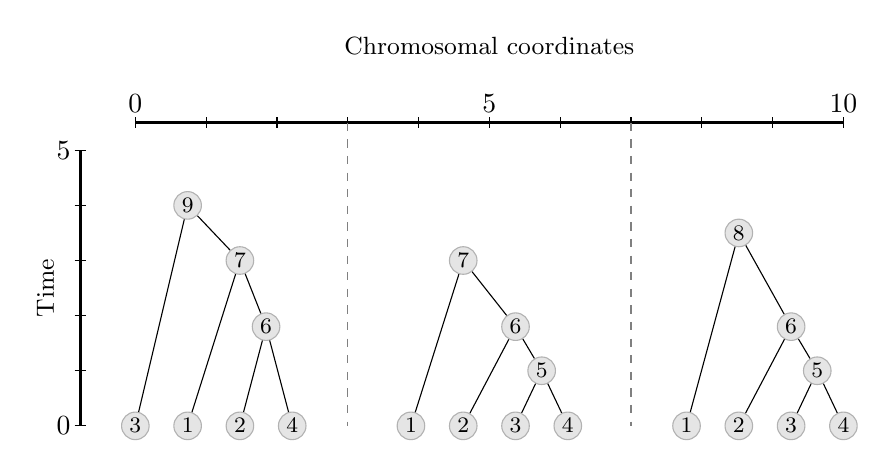
\begin{tikzpicture}[node distance=3mm and 3mm,scale=.7]

\tikzset{greynode/.style={font=\footnotesize,node distance=1cm and 1 cm,fill=black!10,draw=black!30,inner sep=0pt,minimum size=3.5mm,shape=circle},
mutations/.style={shape=starburst,fill=red!50!blue,inner sep=0.8pt,starburst points=11,starburst point height=.2cm}}

% Middle sample nodes
\node (s1) [greynode] {1};
\node (s2) [right=of s1,greynode] {2};
\node (s3) [right=of s2,greynode] {3};
\node (s4) [right=of s3,greynode] {4};

% Left sample nodes
\node (leftTree) at (-5, 0) {};
\node[greynode] (s3l) at ($(s1) + (leftTree)$) {3};
\node[greynode] (s1l) at ($(s2) + (leftTree)$) {1};
\node[greynode] (s2l) at ($(s3) + (leftTree)$) {2};
\node[greynode] (s4l) at ($(s4) + (leftTree)$) {4};

% Right sample nodes
\node (rightTree) at (5, 0) {};
\node [greynode] (s1r) at ($(s1) + (rightTree)$) {1};
\node [greynode] (s2r) at ($(s2) + (rightTree)$) {2};
\node [greynode] (s3r) at ($(s3) + (rightTree)$) {3};
\node [greynode] (s4r) at ($(s4) + (rightTree)$) {4};

% Non-sample nodes
\node [greynode] (s5) at ($0.5*(s3) + 0.5*(s4) + (0,1)$) {5};
\node [greynode] (s5r) at ($(s5) + (rightTree)$) {5};
\node [greynode] (s6) at ($(s3) + (0,1.8)$) {6};
\node [greynode] (s6r) at ($(s6) + (rightTree)$) {6};
\node [greynode] (s6l) at ($0.5*(s2l) + 0.5*(s4l) + (0,1.8)$) {6};
\node [greynode] (s7) at ($(s2) + (0,3)$) {7};
\node [greynode] (s7l) at ($(s2l) + (0,3)$) {7};
\node [greynode] (s8r) at ($(s2r) + (0,3.5)$) {8};
\node [greynode] (s9l) at ($(s1l) + (0,4)$) {9};

% Edges 
\draw (s6l) -- (s2l); \draw (s6l) -- (s4l); \draw (s7l) -- (s1l); \draw (s7l) -- (s6l); \draw (s3l) -- (s9l); \draw (s9l) -- (s7l); %tree 1
\draw (s5) -- (s3); \draw (s5) -- (s4); \draw (s6) -- (s2); \draw (s6) -- (s5); \draw (s7) -- (s1); \draw (s7) -- (s6); % tree 2
\draw (s5r) -- (s3r); \draw (s5r) -- (s4r); \draw (s6r) -- (s2r); \draw (s6r) -- (s5r); \draw (s8r) -- (s1r); \draw (s8r) -- (s6r); % tree 3

% Axes
\node (leftAx) at (-6,0) {};
\draw[very thick] (-6,0) -- +(0, 5);
\foreach \y in {0, 1, 2, 3, 4, 5} \draw ($(leftAx) + (-0.1, \y)$) -- ($(leftAx) + (0.1, \y)$); % tick marks
\draw[very thick] ($(s3l) + (0,5.5)$) -- ($(s4r) + (0,5.5)$);
\node (topAx) at (0,5.5) {};
\node (topLeft) at ($(s3l) + (0,5.5)$) {};
\node (genUnit) at ($0.1*(s4r) - 0.1*(s3l)$) {};
\foreach \x in {0, 1, 2, 3, 4, 5, 6, 7, 8, 9, 10} \draw ($(topLeft) + \x*(genUnit) + (0,0.1)$) -- +(0, -0.2); % tick marks
\node[anchor=east] at ($(leftAx)$) {0}; \node[anchor=east] at ($(leftAx) + (0,5)$) {5};
\node[anchor=south] at ($(topLeft)$) {0}; \node[anchor=south] at ($(topLeft) + 5*(genUnit)$) {5}; \node[anchor=south] at ($(topLeft) + 10*(genUnit)$) {10};

% Interval endpoints
\draw[thin,color=black!50,dashed] ($(topLeft) + 3*(genUnit)$) -- +(0, -5.5);
\draw[thin,color=black!50,dashed] ($(topLeft) + 7*(genUnit)$) -- +(0, -5.5);

%% Mutations
%\node[mutations] (m1) at ($(s3l)!0.3!(s9l)$) {};
%\node[mutations] (m2) at ($(s6l)!0.5!(s7l)$) {};
%\node[mutations] (m3) at ($(s2)!0.6!(s6)$) {};
%\node[mutations] (m4) at ($(s3)!0.5!(s5)$) {};
%\node[mutations] (m5) at ($(s5)!0.5!(s6)$) {};
%\node[mutations] (m6) at ($(s6r)!0.5!(s8r)$) {};
%
%\foreach \x in {1.2, 2.5, 3.3, 3.9, 6.4, 8.4} \node[mutations] at ($(topLeft) + \x*(genUnit) + (0, -0.2)$) {};

% Axis titles
\node (topLabel) at ($(topLeft) + 5*(genUnit) + (0,1.4)$) {$\small\textrm{Chromosomal coordinates}$};
\node[rotate=90,anchor=south] (leftLabel) at ($(leftAx) + (-0.3,2.5)$) {$\small\textrm{Time}$};

%% Haplotypes
%\node[font=\footnotesize] (hap1) at ($(topLeft) + (0,5)$) {$\textrm{Sample }1$};
%\node[font=\footnotesize] (hap2) at ($(topLeft) + (0,4)$) {$\textrm{Sample }2$};
%\node[font=\footnotesize] (hap3) at ($(topLeft) + (0,3)$) {$\textrm{Sample }3$};
%\node[font=\footnotesize] (hap4) at ($(topLeft) + (0,2)$) {$\textrm{Sample }4$};
%
%\foreach \x in {1.2, 2.5, 3.3, 3.9, 6.4, 8.4} \node () at ($(hap1) + \x*(genUnit)$) {0};
%\foreach \x in {2.5, 3.9, 6.4} \node () at ($(hap2) + \x*(genUnit)$) {0};
%\foreach \x in {1.2, 3.3, 8.4} \node () at ($(hap2) + \x*(genUnit)$) {1};
%\foreach \x in {1.2, 3.3} \node () at ($(hap3) + \x*(genUnit)$) {0};
%\foreach \x in {2.5, 3.9, 6.4, 8.4} \node () at ($(hap3) + \x*(genUnit)$) {1};
%\foreach \x in {2.5, 3.3, 3.9} \node () at ($(hap4) + \x*(genUnit)$) {0};
%\foreach \x in {1.2, 6.4, 8.4} \node () at ($(hap4) + \x*(genUnit)$) {1};

\end{tikzpicture}

%\vspace{5mm}
%
%{\footnotesize
%\begin{tabularx}{1\textwidth}{p{0.5cm}p{0.8cm}|p{0.8cm}p{0.8cm}p{0.8cm}p{0.8cm}|p{1.5cm}p{1cm}X}
%\toprule
%\multicolumn{2}{c}{\bf Nodes} & \multicolumn{4}{c}{\bf Edges} & \multicolumn{3}{c}{\bf Mutations}\\
%\midrule
%id & time &
%left & right & parent & child &
%location & time & nearest node\\
%\midrule
%1 & 0.0 &
%0.0 & 7.0 & 5 & 3 &
%1.2 & 2.5 & 6 \\
%2 & 0.0 &
%0.0 & 7.0 & 5 & 4 &
%2.5 & 1.2 & 3\\
%3 & 0.0 &
%0.0 & 10.0 & 6 & 2 &
%3.3 & 1.3 & 2\\
%4 & 0.0 &
%0.0 & 3.0 & 6 & 4 &
%3.9 & 0.4 & 3\\
%5 & 1.1 &
%3.0 & 10.0 & 6 & 5 &
%6.4 & 1.4 & 5\\
%6 & 1.8 &
%0.0 & 7.0 & 7 & 1 &
%8.4 & 2.7 & 6 \\
%7 & 3.0 &
%0.0 & 7.0 & 7 & 6 &
%& &\\
%8 & 3.5 &
%1.0 & 10.0 & 8 & 1 &
%& &\\
%9 & 4.0 &
%7.0 & 10.0 & 8 & 6 &
%& &\\
%& & 
%0.0 & 3.0 & 9 & 3 &
%& &\\
%& & 
%0.0 & 3.0 & 9 & 7 &
%& &\\
%\bottomrule
%\end{tabularx}
%}
\end{center}

\end{center}
%\begin{wideitemize}
%\item 
%The set of genealogies over the entire chromosome can be recorded in a \magenta{tree sequence}.
%\end{wideitemize}
\end{frame}

\begin{frame}
\frametitle{Tree sequences can encode haplotypes}
\begin{center}

\begin{center}

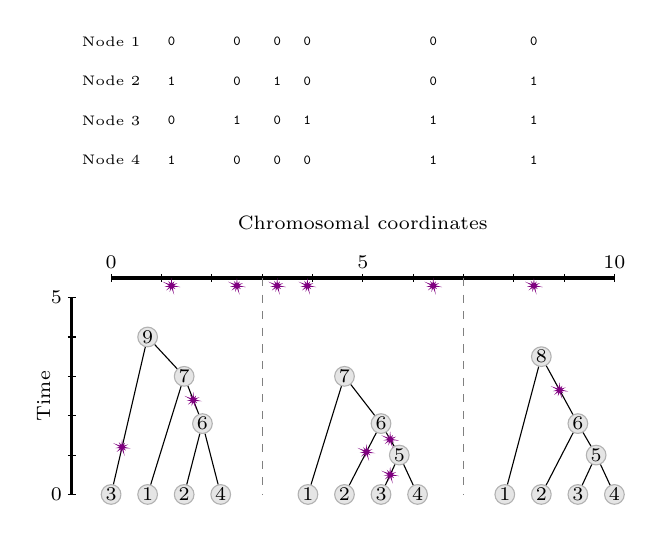
\begin{tikzpicture}[node distance=2mm and 2mm,scale=.5,font=\scriptsize]

\tikzset{greynode/.style={font=\scriptsize,node distance=1cm and 1 cm,fill=black!10,draw=black!30,inner sep=0pt,minimum size=2.5mm,shape=circle},
mutations/.style={shape=starburst,fill=red!50!blue,inner sep=0.6pt,starburst points=11,starburst point height=.1cm}}

% Middle sample nodes
\node (s1) [greynode] {1};
\node (s2) [right=of s1,greynode] {2};
\node (s3) [right=of s2,greynode] {3};
\node (s4) [right=of s3,greynode] {4};

% Left sample nodes
\node (leftTree) at (-5, 0) {};
\node[greynode] (s3l) at ($(s1) + (leftTree)$) {3};
\node[greynode] (s1l) at ($(s2) + (leftTree)$) {1};
\node[greynode] (s2l) at ($(s3) + (leftTree)$) {2};
\node[greynode] (s4l) at ($(s4) + (leftTree)$) {4};

% Right sample nodes
\node (rightTree) at (5, 0) {};
\node [greynode] (s1r) at ($(s1) + (rightTree)$) {1};
\node [greynode] (s2r) at ($(s2) + (rightTree)$) {2};
\node [greynode] (s3r) at ($(s3) + (rightTree)$) {3};
\node [greynode] (s4r) at ($(s4) + (rightTree)$) {4};

% Non-sample nodes
\node [greynode] (s5) at ($0.5*(s3) + 0.5*(s4) + (0,1)$) {5};
\node [greynode] (s5r) at ($(s5) + (rightTree)$) {5};
\node [greynode] (s6) at ($(s3) + (0,1.8)$) {6};
\node [greynode] (s6r) at ($(s6) + (rightTree)$) {6};
\node [greynode] (s6l) at ($0.5*(s2l) + 0.5*(s4l) + (0,1.8)$) {6};
\node [greynode] (s7) at ($(s2) + (0,3)$) {7};
\node [greynode] (s7l) at ($(s2l) + (0,3)$) {7};
\node [greynode] (s8r) at ($(s2r) + (0,3.5)$) {8};
\node [greynode] (s9l) at ($(s1l) + (0,4)$) {9};

% Edges 
\draw (s6l) -- (s2l); \draw (s6l) -- (s4l); \draw (s7l) -- (s1l); \draw (s7l) -- (s6l); \draw (s3l) -- (s9l); \draw (s9l) -- (s7l); %tree 1
\draw (s5) -- (s3); \draw (s5) -- (s4); \draw (s6) -- (s2); \draw (s6) -- (s5); \draw (s7) -- (s1); \draw (s7) -- (s6); % tree 2
\draw (s5r) -- (s3r); \draw (s5r) -- (s4r); \draw (s6r) -- (s2r); \draw (s6r) -- (s5r); \draw (s8r) -- (s1r); \draw (s8r) -- (s6r); % tree 3

% Axes
\node (leftAx) at (-6,0) {};
\draw[very thick] (-6,0) -- +(0, 5);
\foreach \y in {0, 1, 2, 3, 4, 5} \draw ($(leftAx) + (-0.1, \y)$) -- ($(leftAx) + (0.1, \y)$); % tick marks
\draw[very thick] ($(s3l) + (0,5.5)$) -- ($(s4r) + (0,5.5)$);
\node (topAx) at (0,5.5) {};
\node (topLeft) at ($(s3l) + (0,5.5)$) {};
\node (genUnit) at ($0.1*(s4r) - 0.1*(s3l)$) {};
\foreach \x in {0, 1, 2, 3, 4, 5, 6, 7, 8, 9, 10} \draw ($(topLeft) + \x*(genUnit) + (0,0.1)$) -- +(0, -0.2); % tick marks
\node[anchor=east] at ($(leftAx)$) {0}; \node[anchor=east] at ($(leftAx) + (0,5)$) {5};
\node[anchor=south] at ($(topLeft)$) {0}; \node[anchor=south] at ($(topLeft) + 5*(genUnit)$) {5}; \node[anchor=south] at ($(topLeft) + 10*(genUnit)$) {10};

% Interval endpoints
\draw[thin,color=black!50,dashed] ($(topLeft) + 3*(genUnit)$) -- +(0, -5.5);
\draw[thin,color=black!50,dashed] ($(topLeft) + 7*(genUnit)$) -- +(0, -5.5);

% Mutations
\node[mutations] (m1) at ($(s3l)!0.3!(s9l)$) {};
\node[mutations] (m2) at ($(s6l)!0.5!(s7l)$) {};
\node[mutations] (m3) at ($(s2)!0.6!(s6)$) {};
\node[mutations] (m4) at ($(s3)!0.5!(s5)$) {};
\node[mutations] (m5) at ($(s5)!0.5!(s6)$) {};
\node[mutations] (m6) at ($(s6r)!0.5!(s8r)$) {};

\foreach \x in {1.2, 2.5, 3.3, 3.9, 6.4, 8.4} \node[mutations] at ($(topLeft) + \x*(genUnit) + (0, -0.2)$) {};

% Axis titles
\node (topLabel) at ($(topLeft) + 5*(genUnit) + (0,1.4)$) {\scriptsize$\textrm{Chromosomal coordinates}$};
\node[rotate=90,anchor=south] (leftLabel) at ($(leftAx) + (-0.3,2.5)$) {\scriptsize$\textrm{Time}$};

% Haplotypes
\node[font=\footnotesize] (hap1) at ($(topLeft) + (0,6)$) {\tiny$\textrm{Node }1$};
\node[font=\footnotesize] (hap2) at ($(topLeft) + (0,5)$) {\tiny$\textrm{Node }2$};
\node[font=\footnotesize] (hap3) at ($(topLeft) + (0,4)$) {\tiny$\textrm{Node }3$};
\node[font=\footnotesize] (hap4) at ($(topLeft) + (0,3)$) {\tiny$\textrm{Node }4$};

\foreach \x in {1.2, 2.5, 3.3, 3.9, 6.4, 8.4} \node () at ($(hap1) + \x*(genUnit)$) {\tiny \texttt{0}};
\foreach \x in {2.5, 3.9, 6.4} \node () at ($(hap2) + \x*(genUnit)$) {\tiny \texttt{0}};
\foreach \x in {1.2, 3.3, 8.4} \node () at ($(hap2) + \x*(genUnit)$) {\tiny \texttt{1}};
\foreach \x in {1.2, 3.3} \node () at ($(hap3) + \x*(genUnit)$) {\tiny \texttt{0}};
\foreach \x in {2.5, 3.9, 6.4, 8.4} \node () at ($(hap3) + \x*(genUnit)$) {\tiny \texttt{1}};
\foreach \x in {2.5, 3.3, 3.9} \node () at ($(hap4) + \x*(genUnit)$) {\tiny \texttt{0}};
\foreach \x in {1.2, 6.4, 8.4} \node () at ($(hap4) + \x*(genUnit)$) {\tiny \texttt{1}};

\end{tikzpicture}

%\vspace{5mm}
%
%{\footnotesize
%\begin{tabularx}{1\textwidth}{p{0.5cm}p{0.8cm}|p{0.8cm}p{0.8cm}p{0.8cm}p{0.8cm}|p{1.5cm}p{1cm}X}
%\toprule
%\multicolumn{2}{c}{\bf Nodes} & \multicolumn{4}{c}{\bf Edges} & \multicolumn{3}{c}{\bf Mutations}\\
%\midrule
%id & time &
%left & right & parent & child &
%location & time & nearest node\\
%\midrule
%1 & 0.0 &
%0.0 & 7.0 & 5 & 3 &
%1.2 & 2.5 & 6 \\
%2 & 0.0 &
%0.0 & 7.0 & 5 & 4 &
%2.5 & 1.2 & 3\\
%3 & 0.0 &
%0.0 & 10.0 & 6 & 2 &
%3.3 & 1.3 & 2\\
%4 & 0.0 &
%0.0 & 3.0 & 6 & 4 &
%3.9 & 0.4 & 3\\
%5 & 1.1 &
%3.0 & 10.0 & 6 & 5 &
%6.4 & 1.4 & 5\\
%6 & 1.8 &
%0.0 & 7.0 & 7 & 1 &
%8.4 & 2.7 & 6 \\
%7 & 3.0 &
%0.0 & 7.0 & 7 & 6 &
%& &\\
%8 & 3.5 &
%1.0 & 10.0 & 8 & 1 &
%& &\\
%9 & 4.0 &
%7.0 & 10.0 & 8 & 6 &
%& &\\
%& & 
%0.0 & 3.0 & 9 & 3 &
%& &\\
%& & 
%0.0 & 3.0 & 9 & 7 &
%& &\\
%\bottomrule
%\end{tabularx}
%}
\end{center}

\end{center}
\end{frame}

\begin{frame}
\frametitle{Tree sequences can hold info on local ancestry}
\begin{minipage}{.38\textwidth}
\begin{center}


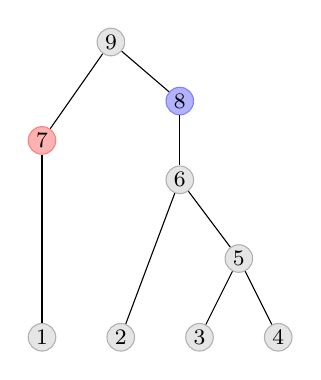
\begin{tikzpicture}[node distance=5mm and 5mm]

\tikzset{greynode/.style={font=\footnotesize,node distance=1cm and 1 cm,fill=black!10,draw=black!30,inner sep=0pt,minimum size=3.5mm,shape=circle},
rednode/.style={font=\footnotesize,node distance=1cm and 1 cm,fill=red!30,draw=red!50,inner sep=0pt,minimum size=3.5mm,shape=circle},
bluenode/.style={font=\footnotesize,node distance=1cm and 1 cm,fill=blue!30,draw=blue!50,inner sep=0pt,minimum size=3.5mm,shape=circle}}

% Sample nodes
\node[greynode] (s1) at (0,0) {1};
\node (s2) [greynode,right of=s1] {2};
\node (s3) [greynode,right of=s2] {3};
\node (s4) [greynode,right of=s3] {4};

% Ancestral nodes
\node[greynode] (s5) at ($0.5*(s3)+0.5*(s4)+ (0,1)$) {5};
\node[greynode] (s6) at ($0.5*(s2) + 0.5*(s5) + (0,1.5)$) {6};
\node[rednode] (s7) at ($(s1) + (0,2.5)$) {7};
\node[bluenode] (s8) at ($(s6) + (0,1)$) {8};
\node[greynode] (s9) at ($0.5*(s7) + 0.5*(s8) + (0,1)$) {9};

% Edges
\draw (s5) -- (s3); \draw (s5) -- (s4); \draw (s6) -- (s2); \draw (s6) -- (s5); \draw (s7) -- (s1); \draw (s8) -- (s6); \draw (s9) -- (s7); \draw (s9) -- (s8);

\end{tikzpicture} 

\end{center}
\end{minipage}\hfill
\begin{minipage}{.58\textwidth}
Nodes may be assigned to populations.\\
The branch joining a sample node to an ancestral node shows the sample's ancestry.
\end{minipage}
\end{frame}

%\begin{frame}
%\frametitle{Tree sequences are good, use them}
%\begin{wideitemize}
%\item $>100\times$ smaller than VCF files for simulated datasets!
%\item Quick to load and query
%\item \texttt{tskit}: a collection of software for creating and analysing tree sequence data
%\end{wideitemize}
%\end{frame}

%\begin{frame}
%\frametitle{Tree sequences can be stored in tables}
%\hspace{-1.5cm}
%\begin{minipage}{.48\textwidth}
%\begin{center}
%
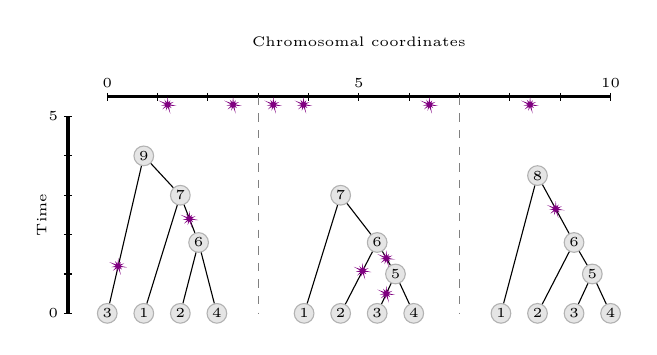
\begin{tikzpicture}[node distance=2mm and 2mm,scale=.5,font=\tiny]

\tikzset{greynode/.style={font=\tiny,node distance=1cm and 1 cm,fill=black!10,draw=black!30,inner sep=0pt,minimum size=2.5mm,shape=circle},
mutations/.style={shape=starburst,fill=red!50!blue,inner sep=0.6pt,starburst points=11,starburst point height=.1cm}}

% Middle sample nodes
\node (s1) [greynode] {1};
\node (s2) [right=of s1,greynode] {2};
\node (s3) [right=of s2,greynode] {3};
\node (s4) [right=of s3,greynode] {4};

% Left sample nodes
\node (leftTree) at (-5, 0) {};
\node[greynode] (s3l) at ($(s1) + (leftTree)$) {3};
\node[greynode] (s1l) at ($(s2) + (leftTree)$) {1};
\node[greynode] (s2l) at ($(s3) + (leftTree)$) {2};
\node[greynode] (s4l) at ($(s4) + (leftTree)$) {4};

% Right sample nodes
\node (rightTree) at (5, 0) {};
\node [greynode] (s1r) at ($(s1) + (rightTree)$) {1};
\node [greynode] (s2r) at ($(s2) + (rightTree)$) {2};
\node [greynode] (s3r) at ($(s3) + (rightTree)$) {3};
\node [greynode] (s4r) at ($(s4) + (rightTree)$) {4};

% Non-sample nodes
\node [greynode] (s5) at ($0.5*(s3) + 0.5*(s4) + (0,1)$) {5};
\node [greynode] (s5r) at ($(s5) + (rightTree)$) {5};
\node [greynode] (s6) at ($(s3) + (0,1.8)$) {6};
\node [greynode] (s6r) at ($(s6) + (rightTree)$) {6};
\node [greynode] (s6l) at ($0.5*(s2l) + 0.5*(s4l) + (0,1.8)$) {6};
\node [greynode] (s7) at ($(s2) + (0,3)$) {7};
\node [greynode] (s7l) at ($(s2l) + (0,3)$) {7};
\node [greynode] (s8r) at ($(s2r) + (0,3.5)$) {8};
\node [greynode] (s9l) at ($(s1l) + (0,4)$) {9};

% Edges 
\draw (s6l) -- (s2l); \draw (s6l) -- (s4l); \draw (s7l) -- (s1l); \draw (s7l) -- (s6l); \draw (s3l) -- (s9l); \draw (s9l) -- (s7l); %tree 1
\draw (s5) -- (s3); \draw (s5) -- (s4); \draw (s6) -- (s2); \draw (s6) -- (s5); \draw (s7) -- (s1); \draw (s7) -- (s6); % tree 2
\draw (s5r) -- (s3r); \draw (s5r) -- (s4r); \draw (s6r) -- (s2r); \draw (s6r) -- (s5r); \draw (s8r) -- (s1r); \draw (s8r) -- (s6r); % tree 3

% Axes
\node (leftAx) at (-6,0) {};
\draw[very thick] (-6,0) -- +(0, 5);
\foreach \y in {0, 1, 2, 3, 4, 5} \draw ($(leftAx) + (-0.1, \y)$) -- ($(leftAx) + (0.1, \y)$); % tick marks
\draw[very thick] ($(s3l) + (0,5.5)$) -- ($(s4r) + (0,5.5)$);
\node (topAx) at (0,5.5) {};
\node (topLeft) at ($(s3l) + (0,5.5)$) {};
\node (genUnit) at ($0.1*(s4r) - 0.1*(s3l)$) {};
\foreach \x in {0, 1, 2, 3, 4, 5, 6, 7, 8, 9, 10} \draw ($(topLeft) + \x*(genUnit) + (0,0.1)$) -- +(0, -0.2); % tick marks
\node[anchor=east] at ($(leftAx)$) {0}; \node[anchor=east] at ($(leftAx) + (0,5)$) {5};
\node[anchor=south] at ($(topLeft)$) {0}; \node[anchor=south] at ($(topLeft) + 5*(genUnit)$) {5}; \node[anchor=south] at ($(topLeft) + 10*(genUnit)$) {10};

% Interval endpoints
\draw[thin,color=black!50,dashed] ($(topLeft) + 3*(genUnit)$) -- +(0, -5.5);
\draw[thin,color=black!50,dashed] ($(topLeft) + 7*(genUnit)$) -- +(0, -5.5);

% Mutations
\node[mutations] (m1) at ($(s3l)!0.3!(s9l)$) {};
\node[mutations] (m2) at ($(s6l)!0.5!(s7l)$) {};
\node[mutations] (m3) at ($(s2)!0.6!(s6)$) {};
\node[mutations] (m4) at ($(s3)!0.5!(s5)$) {};
\node[mutations] (m5) at ($(s5)!0.5!(s6)$) {};
\node[mutations] (m6) at ($(s6r)!0.5!(s8r)$) {};

\foreach \x in {1.2, 2.5, 3.3, 3.9, 6.4, 8.4} \node[mutations] at ($(topLeft) + \x*(genUnit) + (0, -0.2)$) {};

% Axis titles
\node (topLabel) at ($(topLeft) + 5*(genUnit) + (0,1.4)$) {\tiny$\textrm{Chromosomal coordinates}$};
\node[rotate=90,anchor=south] (leftLabel) at ($(leftAx) + (-0.3,2.5)$) {\tiny$\textrm{Time}$};

%% Haplotypes
%\node[font=\footnotesize] (hap1) at ($(topLeft) + (0,6)$) {\tiny$\textrm{Node }1$};
%\node[font=\footnotesize] (hap2) at ($(topLeft) + (0,5)$) {\tiny$\textrm{Node }2$};
%\node[font=\footnotesize] (hap3) at ($(topLeft) + (0,4)$) {\tiny$\textrm{Node }3$};
%\node[font=\footnotesize] (hap4) at ($(topLeft) + (0,3)$) {\tiny$\textrm{Node }4$};
%
%\foreach \x in {1.2, 2.5, 3.3, 3.9, 6.4, 8.4} \node () at ($(hap1) + \x*(genUnit)$) {\tiny \texttt{0}};
%\foreach \x in {2.5, 3.9, 6.4} \node () at ($(hap2) + \x*(genUnit)$) {\tiny \texttt{0}};
%\foreach \x in {1.2, 3.3, 8.4} \node () at ($(hap2) + \x*(genUnit)$) {\tiny \texttt{1}};
%\foreach \x in {1.2, 3.3} \node () at ($(hap3) + \x*(genUnit)$) {\tiny \texttt{0}};
%\foreach \x in {2.5, 3.9, 6.4, 8.4} \node () at ($(hap3) + \x*(genUnit)$) {\tiny \texttt{1}};
%\foreach \x in {2.5, 3.3, 3.9} \node () at ($(hap4) + \x*(genUnit)$) {\tiny \texttt{0}};
%\foreach \x in {1.2, 6.4, 8.4} \node () at ($(hap4) + \x*(genUnit)$) {\tiny \texttt{1}};

\end{tikzpicture}


%\end{center}
%\end{minipage}\hfill
%\begin{minipage}{.48\textwidth}
%\begin{center}
%
{\tiny
\begin{tabularx}{.8\textwidth}{p{0.2cm}p{0.4cm}|p{0.4cm}p{0.4cm}p{0.4cm}X}
\toprule
\multicolumn{2}{c}{\bf Nodes} & \multicolumn{4}{c}{\bf Edges} \\
\midrule
id & time &
left & right & parent & child \\
\midrule
1 & 0.0 &
0.0 & 7.0 & 5 & 3 \\
2 & 0.0 &
0.0 & 7.0 & 5 & 4 \\
3 & 0.0 &
0.0 & 10.0 & 6 & 2 \\
4 & 0.0 &
0.0 & 3.0 & 6 & 4 \\
5 & 1.1 &
3.0 & 10.0 & 6 & 5 \\
6 & 1.8 &
0.0 & 7.0 & 7 & 1 \\
7 & 3.0 &
0.0 & 7.0 & 7 & 6 \\
8 & 3.5 &
1.0 & 10.0 & 8 & 1 \\
9 & 4.0 &
7.0 & 10.0 & 8 & 6 \\
& & 
0.0 & 3.0 & 9 & 3 \\
& & 
0.0 & 3.0 & 9 & 7 \\
%\bottomrule
\end{tabularx}
}\\
{\tiny
\begin{tabularx}{.8\textwidth}{p{.7cm}p{.5cm}X}
\toprule
\multicolumn{3}{c}{\bf Mutations}\\
\midrule
location & time & nearest node\\
\midrule
1.2 & 2.5 & 6 \\
2.5 & 1.2 & 3\\
3.3 & 1.3 & 2\\
3.9 & 0.4 & 3\\
6.4 & 1.4 & 5\\
8.4 & 2.7 & 6 \\
\bottomrule
\end{tabularx}
}


%\end{center}
%\end{minipage}
%\end{frame}

%\begin{frame}
%\frametitle{Local ancestry can be extracted from tree sequences}
%\begin{center}
%
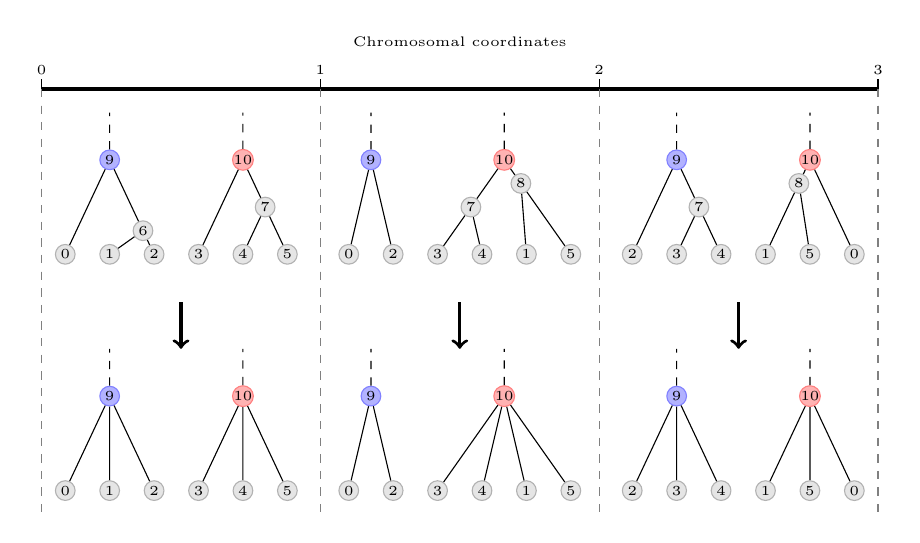
\begin{tikzpicture}[node distance=3mm and 3mm,scale=.6]

\tikzset{greynode/.style={font=\tiny,node distance=.5cm and .5 cm,fill=black!10,draw=black!30,inner sep=0pt,minimum size=2.5mm,shape=circle},
bluenode/.style={font=\tiny,node distance=.5cm and .5cm,fill=blue!30,draw=blue!50,inner sep=0pt,minimum size=2.5mm,shape=circle},
rednode/.style={font=\tiny,node distance=.5cm and .5cm,fill=red!30,draw=red!50,inner sep=0pt,minimum size=2.5mm,shape=circle}}

% Middle sample nodes
\node (s0) [greynode] {0};
\node (s2) [right=of s0,greynode] {2};
\node (s3) [right=of s2,greynode] {3};
\node (s4) [right=of s3,greynode] {4};
\node (s1) [right=of s4,greynode] {1};
\node (s5) [right=of s1,greynode] {5};

% Left sample nodes
\node (leftTree) at (-6, 0) {};
\node[greynode] (s0l) at ($(s0) + (leftTree)$) {0};
\node[greynode] (s1l) at ($(s2) + (leftTree)$) {1};
\node[greynode] (s2l) at ($(s3) + (leftTree)$) {2};
\node[greynode] (s3l) at ($(s4) + (leftTree)$) {3};
\node[greynode] (s4l) at ($(s1) + (leftTree)$) {4};
\node[greynode] (s5l) at ($(s5) + (leftTree)$) {5};

% Right sample nodes
\node (rightTree) at (6, 0) {};
\node [greynode] (s2r) at ($(s0) + (rightTree)$) {2};
\node [greynode] (s3r) at ($(s2) + (rightTree)$) {3};
\node [greynode] (s4r) at ($(s3) + (rightTree)$) {4};
\node [greynode] (s1r) at ($(s4) + (rightTree)$) {1};
\node [greynode] (s5r) at ($(s1) + (rightTree)$) {5};
\node [greynode] (s0r) at ($(s5) + (rightTree)$) {0};

% Ancestral nodes
\node (anc) at (0,2) {};
\node[bluenode] (s9) at ($0.5*(s0) + 0.5*(s2) + (anc)$) {9};
\node[bluenode] (s9l) at ($0.5*(s0l) + 0.5*(s2l) + (anc)$) {9};
\node[bluenode] (s9r) at ($0.5*(s2r) + 0.5*(s4r) + (anc)$) {9};
\node[rednode] (s10) at ($0.5*(s3)+0.5*(s5) + (anc)$) {10};
\node[rednode] (s10l) at ($0.5*(s3l)+0.5*(s5l) + (anc)$) {10};
\node[rednode] (s10r) at ($0.5*(s1r)+0.5*(s0r) + (anc)$) {10};

% Internal nodes
\node[greynode] (s6l) at ($(s2l)!0.25!(s9l)$) {6};
\node[greynode] (s7) at ($(s3)!.5!(s10)$) {7};
\node[greynode] (s7l) at ($(s5l)!.5!(s10l)$) {7};
\node[greynode] (s7r) at ($(s4r)!.5!(s9r)$) {7};
\node[greynode] (s8) at ($(s5)!.75!(s10)$) {8};
\node[greynode] (s8r) at ($(s1r)!.75!(s10r)$) {8};

% Edges
\draw (s0) -- (s9) -- (s2); \draw (s3) -- (s7) -- (s10) -- (s8) -- (s5); \draw (s4) -- (s7); \draw (s1) -- (s8); % middle tree
\draw (s0l) -- (s9l) -- (s6l) -- (s2l); \draw (s1l) -- (s6l); \draw ( s3l) -- (s10l) -- (s7l) -- (s5l); \draw (s4l) -- (s7l); % left tree
\draw (s2r) -- (s9r) -- (s7r) -- (s4r); \draw (s3r) -- (s7r); \draw (s1r) -- (s8r) -- (s10r) -- (s0r); \draw (s5r) -- (s8r); % right tree
\draw[dashed] (s9) -- +(0,1); \draw[dashed] (s9l) -- +(0,1); \draw[dashed] (s9r) -- +(0,1);
\draw[dashed] (s10) -- +(0,1); \draw[dashed] (s10l) -- +(0,1); \draw[dashed] (s10r) -- +(0,1);

% Axes
\node (topAx) at (0,3.5) {};
\node (topLeft) at ($(s0l) + (topAx) + (-0.5, 0)$) {};
\node (topRight) at ($(s0r) + (topAx) + (0.5,0)$) {};
\draw[very thick] (topLeft.center) -- (topRight.center);
\node (genunit) at ($0.3333*(topRight) - 0.3333*(topLeft)$) {};
\foreach \x in {0,1,2,3} \draw ($(topLeft) + \x*(genunit)$) -- +(0,.2);
\foreach \x in {0,1,2,3} \node at ($(topLeft) + \x*(genunit) + (0,.4)$) {\tiny\x};

% Interval endpoints
\foreach \x in {0,1,2,3} \draw[thin,color=black!50,dashed] ($(topLeft) + \x*(genunit)$) -- +(0, -9);
%\draw[thin,color=black!50,dashed] ($(topLeft) + 7*(genUnit)$) -- +(0, -5.5);

% Axis titles
\node (topLabel) at ($(topLeft) + 1.5*(genunit) + (0,1)$) {\tiny$\textrm{Chromosomal coordinates}$};

%%%%%
\node (after) at (0, -5) {};

% Middle sample nodes
\node[greynode] (s0) at (after) {0};
\node (s2) [right=of s0,greynode] {2};
\node (s3) [right=of s2,greynode] {3};
\node (s4) [right=of s3,greynode] {4};
\node (s1) [right=of s4,greynode] {1};
\node (s5) [right=of s1,greynode] {5};

% Left sample nodes
\node (leftTree) at (-6, 0) {};
\node[greynode] (s0l) at ($(s0) + (leftTree)$) {0};
\node[greynode] (s1l) at ($(s2) + (leftTree)$) {1};
\node[greynode] (s2l) at ($(s3) + (leftTree)$) {2};
\node[greynode] (s3l) at ($(s4) + (leftTree)$) {3};
\node[greynode] (s4l) at ($(s1) + (leftTree)$) {4};
\node[greynode] (s5l) at ($(s5) + (leftTree)$) {5};

% Right sample nodes
\node (rightTree) at (6, 0) {};
\node [greynode] (s2r) at ($(s0) + (rightTree)$) {2};
\node [greynode] (s3r) at ($(s2) + (rightTree)$) {3};
\node [greynode] (s4r) at ($(s3) + (rightTree)$) {4};
\node [greynode] (s1r) at ($(s4) + (rightTree)$) {1};
\node [greynode] (s5r) at ($(s1) + (rightTree)$) {5};
\node [greynode] (s0r) at ($(s5) + (rightTree)$) {0};

% Ancestral nodes
\node (anc) at (0,2) {};
\node[bluenode] (s9) at ($0.5*(s0) + 0.5*(s2) + (anc)$) {9};
\node[bluenode] (s9l) at ($0.5*(s0l) + 0.5*(s2l) + (anc)$) {9};
\node[bluenode] (s9r) at ($0.5*(s2r) + 0.5*(s4r) + (anc)$) {9};
\node[rednode] (s10) at ($0.5*(s3)+0.5*(s5) + (anc)$) {10};
\node[rednode] (s10l) at ($0.5*(s3l)+0.5*(s5l) + (anc)$) {10};
\node[rednode] (s10r) at ($0.5*(s1r)+0.5*(s0r) + (anc)$) {10};

%% Axes
%\node (topAx) at (0,3.5) {};
%\node (topLeft) at ($(s0l) + (topAx) + (-0.5, 0)$) {};
%\node (topRight) at ($(s0r) + (topAx) + (0.5,0)$) {};
%\draw[very thick] (topLeft.center) -- (topRight.center);
%\node (genunit) at ($0.3333*(topRight) - 0.3333*(topLeft)$) {};
%\foreach \x in {0,1,2,3} \draw ($(topLeft) + \x*(genunit)$) -- +(0,.2);
%\foreach \x in {0,1,2,3} \node at ($(topLeft) + \x*(genunit) + (0,.4)$) {\x};

% Edges
\draw (s0) -- (s9) -- (s2); \draw (s3) -- (s10) -- (s4); \draw (s1) -- (s10) --  (s5); % middle tree
\draw (s0l) -- (s9l) -- (s2l); \draw (s1l) -- (s9l); \draw (s3l) -- (s10l) -- (s5l); \draw (s4l) -- (s10l); % left tree
\draw (s2r) -- (s9r) -- (s3r); \draw (s4r) -- (s9r); \draw (s1r) -- (s10r) -- (s5r); \draw (s0r) -- (s10r);

\draw[dashed] (s9) -- +(0,1); \draw[dashed] (s9l) -- +(0,1); \draw[dashed] (s9r) -- +(0,1);
\draw[dashed] (s10) -- +(0,1); \draw[dashed] (s10l) -- +(0,1); \draw[dashed] (s10r) -- +(0,1);

% Interval endpoints
\foreach \x in {0,1,2,3} \draw[thin,color=black!50,dashed] ($(topLeft) + \x*(genunit)$) -- +(0, -4);
%\draw[thin,color=black!50,dashed] ($(topLeft) + 7*(genUnit)$) -- +(0, -5.5);

%% Axis titles
%\node (topLabel) at ($(topLeft) + 1.5*(genunit) + (0,1)$) {$\textrm{Chromosomal coordinates}$};

%% Arrows
\foreach \x in {0, 1, 2} \draw[<-,very thick] ($(topLeft) + \x*(genunit) + 0.5*(genunit) + (0,-5.5)$) -- +(0, 1);

\end{tikzpicture}

%\begin{center}
%{\footnotesize
%\begin{tabularx}{1\textwidth}{p{0.5cm}p{0.8cm}|p{0.8cm}p{0.8cm}p{0.8cm}p{0.8cm}|p{1.5cm}p{1cm}X}
%\toprule
%\multicolumn{2}{c}{\bf Nodes} & \multicolumn{4}{c}{\bf Edges} & \multicolumn{3}{c}{\bf Mutations}\\
%\midrule
%id & time &
%left & right & parent & child &
%location & time & nearest node\\
%\midrule
%1 & 0.0 &
%0.0 & 7.0 & 5 & 3 &
%1.2 & 2.5 & 6 \\
%2 & 0.0 &
%0.0 & 7.0 & 5 & 4 &
%2.5 & 1.2 & 3\\
%3 & 0.0 &
%0.0 & 10.0 & 6 & 2 &
%3.3 & 1.3 & 2\\
%4 & 0.0 &
%0.0 & 3.0 & 6 & 4 &
%3.9 & 0.4 & 3\\
%5 & 1.1 &
%3.0 & 10.0 & 6 & 5 &
%6.4 & 1.4 & 5\\
%6 & 1.8 &
%0.0 & 7.0 & 7 & 1 &
%8.4 & 2.7 & 6 \\
%7 & 3.0 &
%0.0 & 7.0 & 7 & 6 &
%& &\\
%8 & 3.5 &
%1.0 & 10.0 & 8 & 1 &
%& &\\
%9 & 4.0 &
%7.0 & 10.0 & 8 & 6 &
%& &\\
%& & 
%0.0 & 3.0 & 9 & 3 &
%& &\\
%& & 
%0.0 & 3.0 & 9 & 7 &
%& &\\
%\bottomrule
%\end{tabularx}
%}
%\end{center}
 

%\end{center}
%\end{frame}

%\begin{frame}
%\frametitle{But doing this efficiently is hard...}
%\begin{wideitemize}
%\item There are substiantial correlations in genealogy between individual nodes, and across genomes.
%\item Requires clever operations for altering tree sequences by `simplifying' the tables that represent them.
%\item More detail in an upcoming paper by Georgia, Damjan, Stephen, Jerome Kelleher (Oxford) \& Peter Ralph (Oregon).
%\end{wideitemize}
%\end{frame}

\section{Simulating admixture: existing methods}

\begin{frame}
\frametitle{\texttt{msprime} simulates \magenta{a sample} backwards-in-time}
\begin{minipage}{.48\textwidth}

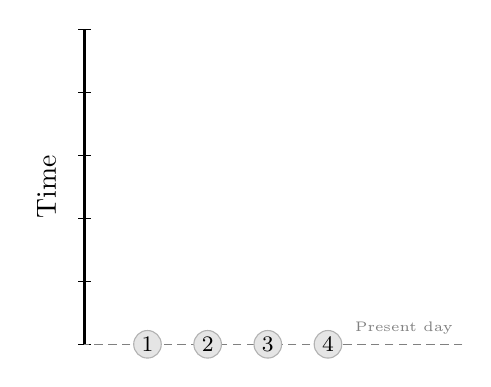
\begin{tikzpicture}[node distance=4mm and 4mm,scale=.8]

\tikzset{greynode/.style={font=\footnotesize,node distance=1cm and 1 cm,fill=black!10,draw=black!30,inner sep=0pt,minimum size=3.5mm,shape=circle},
mutations/.style={shape=starburst,fill=red!50!blue,inner sep=0.8pt,starburst points=11,starburst point height=.2cm}}

% Axis
\node (leftAx) at (-1,0) {};
\draw[very thick] (-1,0) -- +(0, 5);
\foreach \y in {0, 1, 2, 3, 4, 5} \draw ($(leftAx) + (-0.1, \y)$) -- ($(leftAx) + (0.1, \y)$); % tick marks
%\node[anchor=east] at ($(leftAx)$) {0}; \node[anchor=east] at ($(leftAx) + (0,5)$) {5};
\node[rotate=90,anchor=south] (leftLabel) at ($(leftAx) + (-0.3,2.5)$) {$\textrm{Time}$};

% Time arrow
\draw[densely dashed,color=gray] (5,0) node[above left] {\tiny Present day} -- (-1,0);
%\draw[densely dashed,color=gray] (5, 3.6) node[above left] {\tiny Admixture} -- (-1, 3.6);
%\draw[densely dashed,color=gray] (5, 4.5) node[above left] {\tiny Divergence} -- (-1, 4.5);

% sample nodes
\node (s1) [greynode] {1};
\node (s2) [right=of s1,greynode] {2};
\node (s3) [right=of s2,greynode] {3};
\node (s4) [right=of s3,greynode] {4};

% Non-sample nodes
%\node [greynode] (s5) at ($0.5*(s3) + 0.5*(s4) + (0,1.8)$) {5};
%\node [greynode] (s6) at ($0.5*(s2) + 0.5*(s5) + (0,1.5)$) {6};
%\node [greynode] (s7) at ($0.5*(s1) + 0.5*(s6) + (0,2)$) {7};


% Edges 
%\draw (s5) -- (s3); \draw (s5) -- (s4); \draw (s6) -- (s2); \draw (s6) -- (s5); \draw (s7) -- (s1); \draw (s7) -- (s6);

\end{tikzpicture} 

\end{minipage}\hfill
\begin{minipage}{.48\textwidth}
%\begin{wideitemize}
Simulates tree sequences under the coalescent model.\\[5mm]
%\end{wideitemize}
%\gray{\scriptsize Kelleher, J., Etheridge, A. M., \& McVean, G. (2016). Efficient Coalescent Simulation and Genealogical Analysis for Large Sample Sizes. PLOS Computational Biology, 12(5).}
\end{minipage}
\end{frame}

\begin{frame}
\frametitle{\texttt{msprime} simulates \magenta{a sample} backwards-in-time}
\begin{minipage}{.48\textwidth}

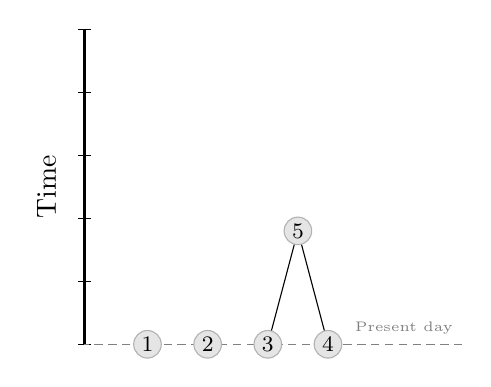
\begin{tikzpicture}[node distance=4mm and 4mm,scale=.8]

\tikzset{greynode/.style={font=\footnotesize,node distance=1cm and 1 cm,fill=black!10,draw=black!30,inner sep=0pt,minimum size=3.5mm,shape=circle},
mutations/.style={shape=starburst,fill=red!50!blue,inner sep=0.8pt,starburst points=11,starburst point height=.2cm}}

% Axis
\node (leftAx) at (-1,0) {};
\draw[very thick] (-1,0) -- +(0, 5);
\foreach \y in {0, 1, 2, 3, 4, 5} \draw ($(leftAx) + (-0.1, \y)$) -- ($(leftAx) + (0.1, \y)$); % tick marks
%\node[anchor=east] at ($(leftAx)$) {0}; \node[anchor=east] at ($(leftAx) + (0,5)$) {5};
\node[rotate=90,anchor=south] (leftLabel) at ($(leftAx) + (-0.3,2.5)$) {$\textrm{Time}$};

% Time arrow
\draw[densely dashed,color=gray] (5,0) node[above left] {\tiny Present day} -- (-1,0);
%\draw[densely dashed,color=gray] (5, 3.6) node[above left] {\tiny Admixture} -- (-1, 3.6);
%\draw[densely dashed,color=gray] (5, 4.5) node[above left] {\tiny Divergence} -- (-1, 4.5);

% sample nodes
\node (s1) [greynode] {1};
\node (s2) [right=of s1,greynode] {2};
\node (s3) [right=of s2,greynode] {3};
\node (s4) [right=of s3,greynode] {4};

% Non-sample nodes
\node [greynode] (s5) at ($0.5*(s3) + 0.5*(s4) + (0,1.8)$) {5};
%\node [greynode] (s6) at ($0.5*(s2) + 0.5*(s5) + (0,1.5)$) {6};
%\node [greynode] (s7) at ($0.5*(s1) + 0.5*(s6) + (0,2)$) {7};


% Edges 
\draw (s5) -- (s3); \draw (s5) -- (s4); %\draw (s6) -- (s2); \draw (s6) -- (s5); \draw (s7) -- (s1); \draw (s7) -- (s6);

\end{tikzpicture} 

\end{minipage}\hfill
\begin{minipage}{.48\textwidth}
%\begin{wideitemize}
Simulates tree sequences under the coalescent model.\\[5mm]
%\end{wideitemize}
%\gray{\scriptsize Kelleher, J., Etheridge, A. M., \& McVean, G. (2016). Efficient Coalescent Simulation and Genealogical Analysis for Large Sample Sizes. PLOS Computational Biology, 12(5).}
\end{minipage}
\end{frame}

\begin{frame}
\frametitle{\texttt{msprime} simulates \magenta{a sample} backwards-in-time}
\begin{minipage}{.48\textwidth}

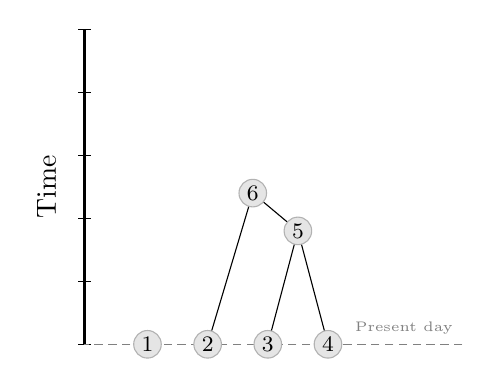
\begin{tikzpicture}[node distance=4mm and 4mm,scale=.8]

\tikzset{greynode/.style={font=\footnotesize,node distance=1cm and 1 cm,fill=black!10,draw=black!30,inner sep=0pt,minimum size=3.5mm,shape=circle},
mutations/.style={shape=starburst,fill=red!50!blue,inner sep=0.8pt,starburst points=11,starburst point height=.2cm}}

% Axis
\node (leftAx) at (-1,0) {};
\draw[very thick] (-1,0) -- +(0, 5);
\foreach \y in {0, 1, 2, 3, 4, 5} \draw ($(leftAx) + (-0.1, \y)$) -- ($(leftAx) + (0.1, \y)$); % tick marks
%\node[anchor=east] at ($(leftAx)$) {0}; \node[anchor=east] at ($(leftAx) + (0,5)$) {5};
\node[rotate=90,anchor=south] (leftLabel) at ($(leftAx) + (-0.3,2.5)$) {$\textrm{Time}$};

% Time arrow
\draw[densely dashed,color=gray] (5,0) node[above left] {\tiny Present day} -- (-1,0);
%\draw[densely dashed,color=gray] (5, 3.6) node[above left] {\tiny Admixture} -- (-1, 3.6);
%\draw[densely dashed,color=gray] (5, 4.5) node[above left] {\tiny Divergence} -- (-1, 4.5);

% sample nodes
\node (s1) [greynode] {1};
\node (s2) [right=of s1,greynode] {2};
\node (s3) [right=of s2,greynode] {3};
\node (s4) [right=of s3,greynode] {4};

% Non-sample nodes
\node [greynode] (s5) at ($0.5*(s3) + 0.5*(s4) + (0,1.8)$) {5};
\node [greynode] (s6) at ($0.5*(s2) + 0.5*(s5) + (0,1.5)$) {6};
%\node [greynode] (s7) at ($0.5*(s1) + 0.5*(s6) + (0,2)$) {7};


% Edges 
\draw (s5) -- (s3); \draw (s5) -- (s4); \draw (s6) -- (s2); \draw (s6) -- (s5); %\draw (s7) -- (s1); \draw (s7) -- (s6);

\end{tikzpicture} 

\end{minipage}\hfill
\begin{minipage}{.48\textwidth}
%\begin{wideitemize}
Simulates tree sequences under the coalescent model.\\[5mm]
%\end{wideitemize}
%\gray{\scriptsize Kelleher, J., Etheridge, A. M., \& McVean, G. (2016). Efficient Coalescent Simulation and Genealogical Analysis for Large Sample Sizes. PLOS Computational Biology, 12(5).}
\end{minipage}
\end{frame}

\begin{frame}
\frametitle{\texttt{msprime} simulates \magenta{a sample} backwards-in-time}
\begin{minipage}{.48\textwidth}

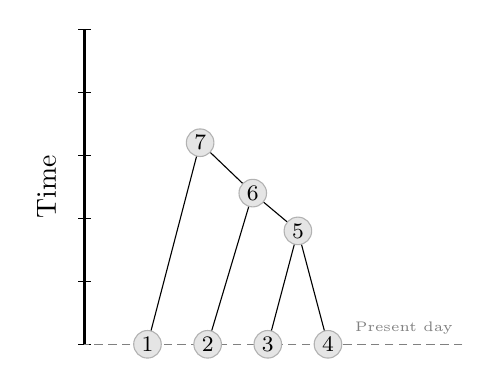
\begin{tikzpicture}[node distance=4mm and 4mm,scale=.8]

\tikzset{greynode/.style={font=\footnotesize,node distance=1cm and 1 cm,fill=black!10,draw=black!30,inner sep=0pt,minimum size=3.5mm,shape=circle},
mutations/.style={shape=starburst,fill=red!50!blue,inner sep=0.8pt,starburst points=11,starburst point height=.2cm}}

% Axis
\node (leftAx) at (-1,0) {};
\draw[very thick] (-1,0) -- +(0, 5);
\foreach \y in {0, 1, 2, 3, 4, 5} \draw ($(leftAx) + (-0.1, \y)$) -- ($(leftAx) + (0.1, \y)$); % tick marks
%\node[anchor=east] at ($(leftAx)$) {0}; \node[anchor=east] at ($(leftAx) + (0,5)$) {5};
\node[rotate=90,anchor=south] (leftLabel) at ($(leftAx) + (-0.3,2.5)$) {$\textrm{Time}$};

% Time arrow
\draw[densely dashed,color=gray] (5,0) node[above left] {\tiny Present day} -- (-1,0);
%\draw[densely dashed,color=gray] (5, 3.6) node[above left] {\tiny Admixture} -- (-1, 3.6);
%\draw[densely dashed,color=gray] (5, 4.5) node[above left] {\tiny Divergence} -- (-1, 4.5);

% sample nodes
\node (s1) [greynode] {1};
\node (s2) [right=of s1,greynode] {2};
\node (s3) [right=of s2,greynode] {3};
\node (s4) [right=of s3,greynode] {4};

% Non-sample nodes
\node [greynode] (s5) at ($0.5*(s3) + 0.5*(s4) + (0,1.8)$) {5};
\node [greynode] (s6) at ($0.5*(s2) + 0.5*(s5) + (0,1.5)$) {6};
\node [greynode] (s7) at ($0.5*(s1) + 0.5*(s6) + (0,2)$) {7};


% Edges 
\draw (s5) -- (s3); \draw (s5) -- (s4); \draw (s6) -- (s2); \draw (s6) -- (s5); \draw (s7) -- (s1); \draw (s7) -- (s6);

\end{tikzpicture} 

\end{minipage}\hfill
\begin{minipage}{.48\textwidth}
%\begin{wideitemize}
Simulates tree sequences under the coalescent model.\\[5mm]
%\end{wideitemize}
%\gray{\scriptsize Kelleher, J., Etheridge, A. M., \& McVean, G. (2016). Efficient Coalescent Simulation and Genealogical Analysis for Large Sample Sizes. PLOS Computational Biology, 12(5).}
\end{minipage}
\end{frame}

\begin{frame}
\frametitle{A simplified toy example: Neanderthal introgression}
\begin{center}
\begin{tabularx}{1\textwidth}{p{3cm}X}
\toprule
{\bf Generations} & {\bf Event}\\
\midrule
$\approx$ 240\ts 000 & Common ancestor of all modern Eurasians and Neanderthals at all loci.\\[1mm]
20\ts 000 & Divergence of Eurasians and Neanderthals.\\[1mm]
2\ts 500 & 2\% introgression of Neanderthals into Eurasians.\\[1mm]
0 & Samples from 100 Eurasian individuals obtained.\\
\bottomrule
\end{tabularx}
\end{center}
Chromosome of 50\ts 000\ts 000 base pairs, constant effective population sizes of 5000 individuals, uniform recombination rate $1\times 10^{-8}$ bp/generation, uniform mutation rate $1\times 10^{-8}$ bp/generation, all variation is neutral.
\end{frame}

\begin{frame}
\frametitle{\texttt{msprime} results: missing ancestry data}
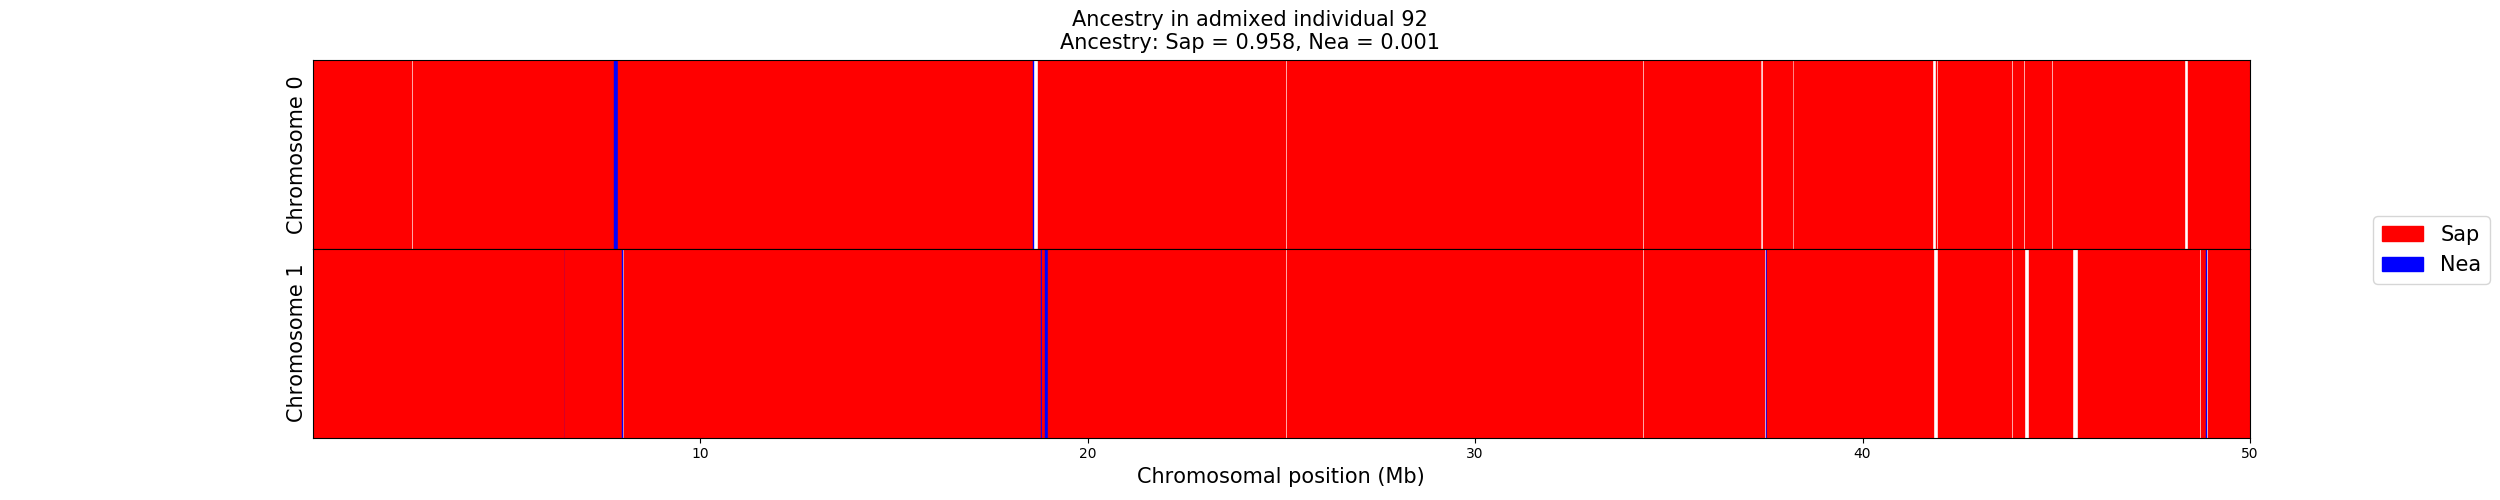
\includegraphics[scale=.22]{pics/msprime/msprime-sample.png}\quad\quad
Global ancestry averaged over all of the simulated samples was 
\begin{itemize}
\item $96.0\%$ Sapiens
\item $<0.05\%$ Neanderthal
\item \magenta{$4.0\%$ unassigned.}
\end{itemize}
%0.960 Sapiens, 0.000 Neanderthal, \magenta{0.040 unassigned.}
\end{frame}

\begin{frame}
\frametitle{Missing ancestry is due to incomplete lineage sorting}
\begin{center}

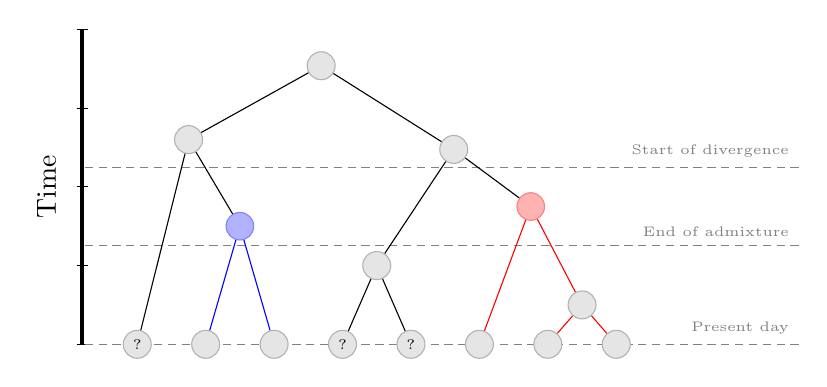
\begin{tikzpicture}[node distance=3mm and 5mm,xscale=.7,yscale=.5]

\tikzset{greynode/.style={font=\tiny,node distance=1cm and 1 cm,fill=black!10,draw=black!30,inner sep=0pt,minimum size=3.55mm,shape=circle},
bluenode/.style={font=\tiny,node distance=1cm and 1 cm,fill=blue!30,draw=blue!50,inner sep=0pt,minimum size=3.5mm,shape=circle},
rednode/.style={font=\tiny,node distance=1cm and 1 cm,fill=red!30,draw=red!50,inner sep=0pt,minimum size=3.5mm,shape=circle}}

% Axis
\node (leftAx) at (-1,0) {};
\draw[very thick] (-1,0) -- +(0, 8);
\foreach \y in {0, 2, 4, 6, 8} \draw ($(leftAx) + (-0.1, \y)$) -- ($(leftAx) + (0.1, \y)$); % tick marks
%\node[anchor=east] at ($(leftAx)$) {0}; \node[anchor=east] at ($(leftAx) + (0,5)$) {5};
\node[rotate=90,anchor=south] (leftLabel) at ($(leftAx) + (-0.3,4)$) {$\textrm{Time}$};

% Time arrow
\draw[densely dashed,color=gray] (12,0) node[above left] {\tiny Present day} -- (-1,0);
\draw[densely dashed,color=gray] (12, 2.5) node[above left] {\tiny End of admixture} -- (-1, 2.5);
\draw[densely dashed,color=gray] (12, 4.5) node[above left] {\tiny Start of divergence} -- (-1, 4.5);

% sample nodes
\node (s1) [greynode] {$\textrm{?}$};
\node (s2) [right=of s1,greynode] {};
\node (s3) [right=of s2,greynode] {};
\node (s4) [right=of s3,greynode] {$\textrm{?}$};
\node (s5) [right=of s4,greynode] {$\textrm{?}$};
\node (s6) [right=of s5,greynode] {};
\node (s7) [right=of s6,greynode] {};
\node (s8) [right=of s7,greynode] {};

% Non-sample nodes
\node[greynode] (s9) at ($0.5*(s7) + 0.5*(s8) + (0,1)$) {};
\node[greynode] (s10) at ($0.5*(s4) + 0.5*(s5) + (0,2)$) {};
\node[bluenode] (s11) at ($0.5*(s2)+0.5*(s3) + (0,3)$) {};
\node[rednode] (s12) at ($0.5*(s9)+0.5*(s6) +(0,3)$) {};
\node[greynode] (s13) at ($0.5*(s10)+0.5*(s12) + (0,2.2)$) {};
\node[greynode] (s14) at ($0.5*(s1)+0.5*(s11)+(0,3.7)$) {};
\node[greynode] (s15) at ($0.5*(s13) + 0.5*(s14) + (0,2)$) {};

% Coloured edges
\foreach \x in {2,3} \draw[color=blue] (s\x) -- (s11); 
\foreach \x in {7,8} \draw[color=red] (s\x) -- (s9);
\foreach \x in {6,9} \draw[color=red] (s\x) -- (s12);

% Black edges
\foreach \x in {4,5} \draw (s\x) -- (s10);
\foreach \x in {10,12} \draw (s\x) -- (s13);
\foreach \x in {1,11} \draw (s\x) -- (s14);
\foreach \x in {13,14} \draw (s\x) -- (s15);

\end{tikzpicture} 

\end{center}
Some samples do not have simulated ancestors in the given populations.
\end{frame}

\begin{frame}
\frametitle{\texttt{msprime} performance}
\begin{center}
\small
\centering
\setlength{\aboverulesep}{5pt}
\setlength{\belowrulesep}{5pt}
\begin{tabularx}{1\textwidth}{p{3.5cm}p{2cm}p{1.9cm}p{1.9cm}X}
\toprule
%& \multicolumn{3}{c}{{\bf Global ancestry}} \\[1mm]
 & Missing data & Run time & File size & Realism \\
\midrule 
{\bf default} & $4.0$\% & 6 sec &  9 Mb & \crossmark \\ \addlinespace
{\bf + all ancestors} & $0.0$\% & 53 sec  &  1700 Mb & \crossmark \\ \addlinespace
%{\bf + migration records} & $0.0$\% &  & & \crossmark \\ \addlinespace
\bottomrule
\end{tabularx}
\end{center}
\vspace{5mm}
Restricted by the limitations of the coalescent model: no selection, random mating, small sample sizes, no more than 1 mutation at any location \ldots
\end{frame}

%\begin{frame}
%\frametitle{}
%\begin{wideitemize}
%\item \texttt{msprime} simulates the sparsest set of haplotypes that are needed to represent the relative genealogical history of the samples.
%\item This sparsity makes it quick and memory-efficient to run.
%\item Limited by the assumptions of the coalescent model: infinite sites, no selection or deviations from random mating, small sample size relative to effective population size...
%\item See (Kelleher et al., 2016) for more details.
%\end{wideitemize}
%\end{frame}

\begin{frame}
\frametitle{\texttt{SLiM} simulates \magenta{an entire population} forward-in-time}
\begin{minipage}{.58\textwidth}

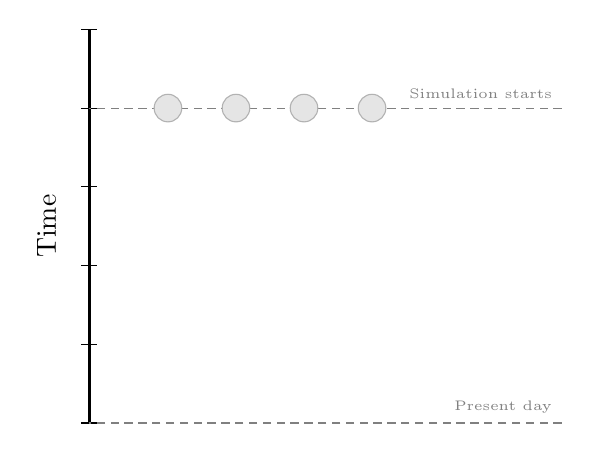
\begin{tikzpicture}[node distance=5mm and 5mm]

\tikzset{greynode/.style={font=\footnotesize,node distance=1cm and 1 cm,fill=black!10,draw=black!30,inner sep=0pt,minimum size=3.5mm,shape=circle},
mutations/.style={shape=starburst,fill=red!50!blue,inner sep=0.8pt,starburst points=11,starburst point height=.2cm}}

\node (timestart) at (0,-4) {};

% Axis
\node (leftAx) at ($(-1,0) + (timestart)$) {};
\draw[very thick] ($(-1,0) + (timestart)$) -- +(0, 5);
\foreach \y in {0, 1, 2, 3, 4, 5} \draw ($(leftAx) + (-0.1, \y)$) -- ($(leftAx) + (0.1, \y)$); % tick marks
%\node[anchor=east] at ($(leftAx)$) {0}; \node[anchor=east] at ($(leftAx) + (0,5)$) {5};
\node[rotate=90,anchor=south] (leftLabel) at ($(leftAx) + (-0.3,2.5)$) {$\textrm{Time}$};

% Time arrow
\draw[densely dashed,color=gray] ($(5,0) + (timestart)$) node[above left] {\tiny Present day} -- ($(-1,0) + (timestart)$);
\draw[densely dashed,color=gray] ($(5,4) + (timestart)$) node[above left] {\tiny Simulation starts} -- ($(-1,4) + (timestart)$);

% sample nodes
\node (s1) [greynode] {};
\node (s2) [right=of s1,greynode] {};
\node (s3) [right=of s2,greynode] {};
\node (s4) [right=of s3,greynode] {};

% Non-sample nodes
%\foreach \x in {1,2,3,4} \foreach \y in {1,2,3,4} \node[greynode] (s\x\y) at ($(s\x) + (0,-\y)$) {};


% Edges 


\end{tikzpicture} 

\end{minipage}\hfill
\begin{minipage}{.4\textwidth}
Alternates between
\begin{enumerate}
\item forward simulation
\item pruning of irrelevant history.
\end{enumerate}
\end{minipage}
\end{frame}

%\begin{frame}
%\frametitle{\texttt{SLiM} simulates \magenta{an entire population} forward-in-time}
%\begin{minipage}{.58\textwidth}
%
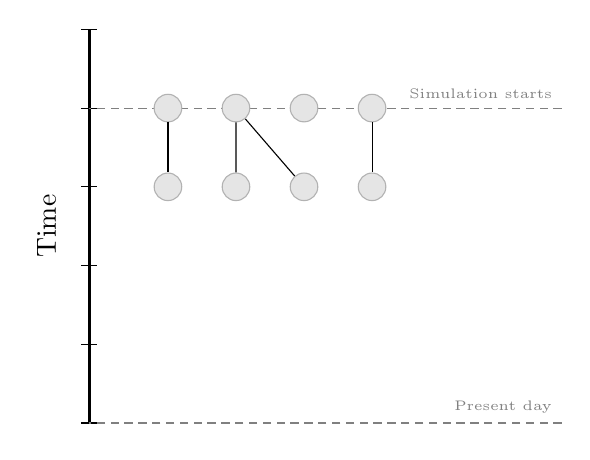
\begin{tikzpicture}[node distance=5mm and 5mm]

\tikzset{greynode/.style={font=\footnotesize,node distance=1cm and 1 cm,fill=black!10,draw=black!30,inner sep=0pt,minimum size=3.5mm,shape=circle},
mutations/.style={shape=starburst,fill=red!50!blue,inner sep=0.8pt,starburst points=11,starburst point height=.2cm}}

\node (timestart) at (0,-4) {};

% Axis
\node (leftAx) at ($(-1,0) + (timestart)$) {};
\draw[very thick] ($(-1,0) + (timestart)$) -- +(0, 5);
\foreach \y in {0, 1, 2, 3, 4, 5} \draw ($(leftAx) + (-0.1, \y)$) -- ($(leftAx) + (0.1, \y)$); % tick marks
%\node[anchor=east] at ($(leftAx)$) {0}; \node[anchor=east] at ($(leftAx) + (0,5)$) {5};
\node[rotate=90,anchor=south] (leftLabel) at ($(leftAx) + (-0.3,2.5)$) {$\textrm{Time}$};

% Time arrow
\draw[densely dashed,color=gray] ($(5,0) + (timestart)$) node[above left] {\tiny Present day} -- ($(-1,0) + (timestart)$);
\draw[densely dashed,color=gray] ($(5,4) + (timestart)$) node[above left] {\tiny Simulation starts} -- ($(-1,4) + (timestart)$);

% sample nodes
\node (s1) [greynode] {};
\node (s2) [right=of s1,greynode] {};
\node (s3) [right=of s2,greynode] {};
\node (s4) [right=of s3,greynode] {};

% Non-sample nodes
\foreach \x in {1,2,3,4} \foreach \y in {1} \node[greynode] (s\x\y) at ($(s\x) + (0,-\y)$) {};

% Edges 
\draw (s1) -- (s11); \draw (s21) -- (s2) -- (s31); \draw (s4) -- (s41);


\end{tikzpicture} 

%\end{minipage}\hfill
%\begin{minipage}{.4\textwidth}
%Alternates between
%\begin{enumerate}
%\item \magenta{forward simulation}
%\item pruning of irrelevant history.
%\end{enumerate}
%\end{minipage}
%\end{frame}

\begin{frame}
\frametitle{\texttt{SLiM} simulates \magenta{an entire population} forward-in-time}
\begin{minipage}{.58\textwidth}

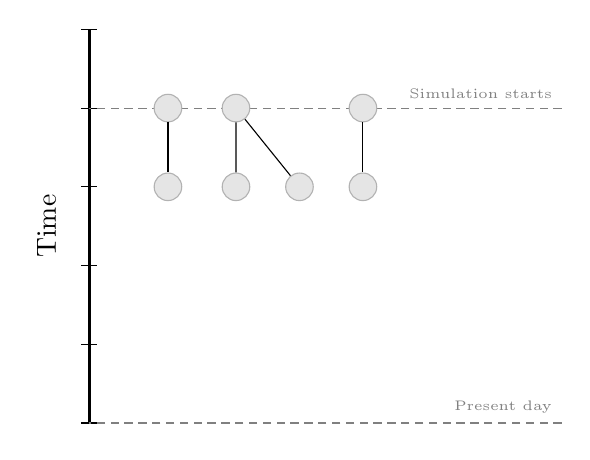
\begin{tikzpicture}[node distance=5mm and 5mm]

\tikzset{greynode/.style={font=\footnotesize,node distance=1cm and 1 cm,fill=black!10,draw=black!30,inner sep=0pt,minimum size=3.5mm,shape=circle},
mutations/.style={shape=starburst,fill=red!50!blue,inner sep=0.8pt,starburst points=11,starburst point height=.2cm}}

\node (timestart) at (0,-4) {};

% Axis
\node (leftAx) at ($(-1,0) + (timestart)$) {};
\draw[very thick] ($(-1,0) + (timestart)$) -- +(0, 5);
\foreach \y in {0, 1, 2, 3, 4, 5} \draw ($(leftAx) + (-0.1, \y)$) -- ($(leftAx) + (0.1, \y)$); % tick marks
%\node[anchor=east] at ($(leftAx)$) {0}; \node[anchor=east] at ($(leftAx) + (0,5)$) {5};
\node[rotate=90,anchor=south] (leftLabel) at ($(leftAx) + (-0.3,2.5)$) {$\textrm{Time}$};

% Time arrow
\draw[densely dashed,color=gray] ($(5,0) + (timestart)$) node[above left] {\tiny Present day} -- ($(-1,0) + (timestart)$);
\draw[densely dashed,color=gray] ($(5,4) + (timestart)$) node[above left] {\tiny Simulation starts} -- ($(-1,4) + (timestart)$);

% sample nodes
\node (s1) [greynode] {};
\node (s2) [right=of s1,greynode] {};
\node (s3) [right=of s2] {};
\node (s4) [right=of s3,greynode] {};

% Non-sample nodes
\foreach \x in {1,2,3,4} \foreach \y in {1} \node[greynode] (s\x\y) at ($(s\x) + (0,-\y)$) {};

% Edges 
\draw (s1) -- (s11); \draw (s21) -- (s2) -- (s31); \draw (s4) -- (s41);


\end{tikzpicture} 

\end{minipage}\hfill
\begin{minipage}{.4\textwidth}
Alternates between
\begin{enumerate}
\item forward simulation
\item pruning of irrelevant history.
\end{enumerate}
\end{minipage}
\end{frame}

%\begin{frame}
%\frametitle{\texttt{SLiM} simulates \magenta{an entire population} forward-in-time}
%\begin{minipage}{.58\textwidth}
%
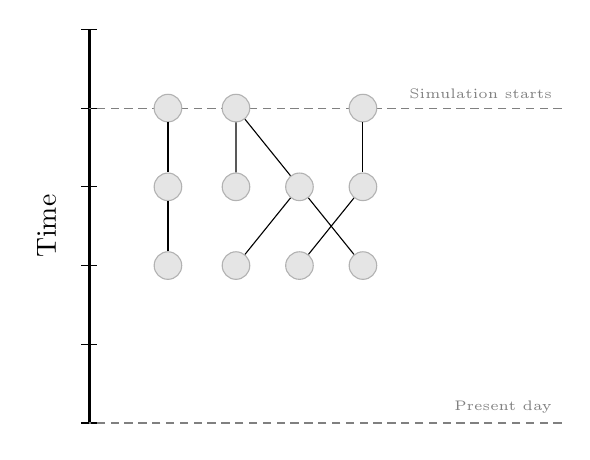
\begin{tikzpicture}[node distance=5mm and 5mm]

\tikzset{greynode/.style={font=\footnotesize,node distance=1cm and 1 cm,fill=black!10,draw=black!30,inner sep=0pt,minimum size=3.5mm,shape=circle},
whitenode/.style={font=\footnotesize,node distance=1cm and 1 cm,fill=white,draw=white,inner sep=0pt,minimum size=3.7mm,shape=circle},
mutations/.style={shape=starburst,fill=red!50!blue,inner sep=0.8pt,starburst points=11,starburst point height=.2cm}}

\node (timestart) at (0,-4) {};

% Axis
\node (leftAx) at ($(-1,0) + (timestart)$) {};
\draw[very thick] ($(-1,0) + (timestart)$) -- +(0, 5);
\foreach \y in {0, 1, 2, 3, 4, 5} \draw ($(leftAx) + (-0.1, \y)$) -- ($(leftAx) + (0.1, \y)$); % tick marks
%\node[anchor=east] at ($(leftAx)$) {0}; \node[anchor=east] at ($(leftAx) + (0,5)$) {5};
\node[rotate=90,anchor=south] (leftLabel) at ($(leftAx) + (-0.3,2.5)$) {$\textrm{Time}$};

% Time arrow
\draw[densely dashed,color=gray] ($(5,0) + (timestart)$) node[above left] {\tiny Present day} -- ($(-1,0) + (timestart)$);
\draw[densely dashed,color=gray] ($(5,4) + (timestart)$) node[above left] {\tiny Simulation starts} -- ($(-1,4) + (timestart)$);

% sample nodes
\node (s1) [greynode] {};
\node (s2) [right=of s1,greynode] {};
\node (s3) [right=of s2] {};
\node (s4) [right=of s3,greynode] {};

% Non-sample nodes
\foreach \x in {1,2,3,4} \foreach \y in {1,2} \node[greynode] (s\x\y) at ($(s\x) + (0,-\y)$) {};

% Edges 
\draw (s1) -- (s11); \draw (s21) -- (s2) -- (s31); \draw (s4) -- (s41);
\draw (s11) -- (s12); \draw (s22) -- (s31) -- (s42); \draw (s41) -- (s32);

% Remove some nodes
%\node[whitenode] at (s3) {};

\end{tikzpicture} 

%\end{minipage}\hfill
%\begin{minipage}{.4\textwidth}
%Alternates between
%\begin{enumerate}
%\item \magenta{forward simulation}
%\item pruning of irrelevant history.
%\end{enumerate}
%\end{minipage}
%\end{frame}

\begin{frame}
\frametitle{\texttt{SLiM} simulates \magenta{an entire population} forward-in-time}
\begin{minipage}{.58\textwidth}

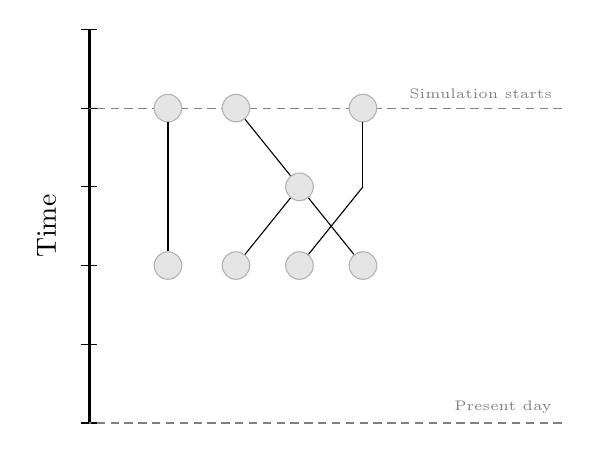
\begin{tikzpicture}[node distance=5mm and 5mm]

\tikzset{greynode/.style={font=\footnotesize,node distance=1cm and 1 cm,fill=black!10,draw=black!30,inner sep=0pt,minimum size=3.5mm,shape=circle},
whitenode/.style={font=\footnotesize,node distance=1cm and 1 cm,fill=white,draw=white,inner sep=0pt,minimum size=3.7mm,shape=circle},
mutations/.style={shape=starburst,fill=red!50!blue,inner sep=0.8pt,starburst points=11,starburst point height=.2cm}}

\node (timestart) at (0,-4) {};

% Axis
\node (leftAx) at ($(-1,0) + (timestart)$) {};
\draw[very thick] ($(-1,0) + (timestart)$) -- +(0, 5);
\foreach \y in {0, 1, 2, 3, 4, 5} \draw ($(leftAx) + (-0.1, \y)$) -- ($(leftAx) + (0.1, \y)$); % tick marks
%\node[anchor=east] at ($(leftAx)$) {0}; \node[anchor=east] at ($(leftAx) + (0,5)$) {5};
\node[rotate=90,anchor=south] (leftLabel) at ($(leftAx) + (-0.3,2.5)$) {$\textrm{Time}$};

% Time arrow
\draw[densely dashed,color=gray] ($(5,0) + (timestart)$) node[above left] {\tiny Present day} -- ($(-1,0) + (timestart)$);
\draw[densely dashed,color=gray] ($(5,4) + (timestart)$) node[above left] {\tiny Simulation starts} -- ($(-1,4) + (timestart)$);

% sample nodes
\node (s1) [greynode] {};
\node (s2) [right=of s1,greynode] {};
\node (s3) [right=of s2] {};
\node (s4) [right=of s3,greynode] {};

% Non-sample nodes
\foreach \x in {1,2,3,4} \foreach \y in {1,2} \node[greynode] (s\x\y) at ($(s\x) + (0,-\y)$) {};

% Remove some nodes
\node[whitenode] at (s21) {}; \node[whitenode] at (s11) {}; \node[whitenode] at (s41){};

% Edges 
\draw (s1) -- (s11.center); \draw (s2) -- (s31); \draw (s4) -- (s41.center);
\draw (s11.center) -- (s12); \draw (s22) -- (s31) -- (s42); \draw (s41.center) -- (s32);
%\draw (s13) -- (s22) -- (s33); \draw (s23) -- (s32) -- (s43);

\end{tikzpicture} 

\end{minipage}\hfill
\begin{minipage}{.4\textwidth}
Alternates between
\begin{enumerate}
\item forward simulation
\item pruning of irrelevant history.
\end{enumerate}
\end{minipage}
\end{frame}

%\begin{frame}
%\frametitle{\texttt{SLiM} simulates \magenta{an entire population} forward-in-time}
%\begin{minipage}{.58\textwidth}
%
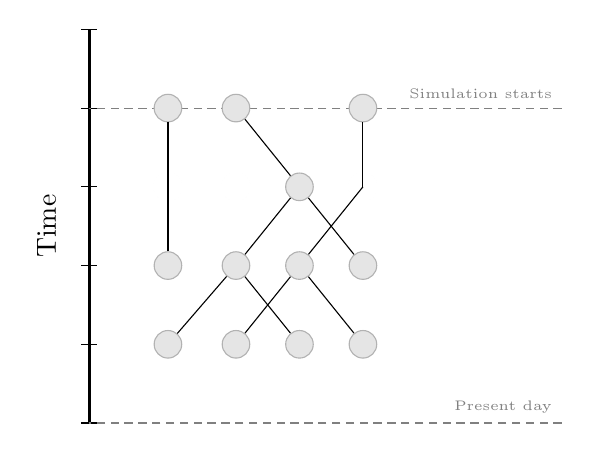
\begin{tikzpicture}[node distance=5mm and 5mm]

\tikzset{greynode/.style={font=\footnotesize,node distance=1cm and 1 cm,fill=black!10,draw=black!30,inner sep=0pt,minimum size=3.5mm,shape=circle},
whitenode/.style={font=\footnotesize,node distance=1cm and 1 cm,fill=white,draw=white,inner sep=0pt,minimum size=3.7mm,shape=circle},
mutations/.style={shape=starburst,fill=red!50!blue,inner sep=0.8pt,starburst points=11,starburst point height=.2cm}}

\node (timestart) at (0,-4) {};

% Axis
\node (leftAx) at ($(-1,0) + (timestart)$) {};
\draw[very thick] ($(-1,0) + (timestart)$) -- +(0, 5);
\foreach \y in {0, 1, 2, 3, 4, 5} \draw ($(leftAx) + (-0.1, \y)$) -- ($(leftAx) + (0.1, \y)$); % tick marks
%\node[anchor=east] at ($(leftAx)$) {0}; \node[anchor=east] at ($(leftAx) + (0,5)$) {5};
\node[rotate=90,anchor=south] (leftLabel) at ($(leftAx) + (-0.3,2.5)$) {$\textrm{Time}$};

% Time arrow
\draw[densely dashed,color=gray] ($(5,0) + (timestart)$) node[above left] {\tiny Present day} -- ($(-1,0) + (timestart)$);
\draw[densely dashed,color=gray] ($(5,4) + (timestart)$) node[above left] {\tiny Simulation starts} -- ($(-1,4) + (timestart)$);

% sample nodes
\node (s1) [greynode] {};
\node (s2) [right=of s1,greynode] {};
\node (s3) [right=of s2] {};
\node (s4) [right=of s3,greynode] {};

% Non-sample nodes
\foreach \x in {1,2,3,4} \foreach \y in {1,2,3} \node[greynode] (s\x\y) at ($(s\x) + (0,-\y)$) {};

% Remove some nodes
\node[whitenode] at (s21) {}; \node[whitenode] at (s11) {}; \node[whitenode] at (s41){};

% Edges 
\draw (s1) -- (s11.center); \draw (s2) -- (s31); \draw (s4) -- (s41.center);
\draw (s11.center) -- (s12); \draw (s22) -- (s31) -- (s42); \draw (s41.center) -- (s32);
\draw (s13) -- (s22) -- (s33); \draw (s23) -- (s32) -- (s43);

\end{tikzpicture} 

%\end{minipage}\hfill
%\begin{minipage}{.4\textwidth}
%Alternates between
%\begin{enumerate}
%\item \magenta{forward simulation}
%\item pruning of irrelevant history.
%\end{enumerate}
%\end{minipage}
%\end{frame}

\begin{frame}
\frametitle{\texttt{SLiM} simulates \magenta{an entire population} forward-in-time}
\begin{minipage}{.58\textwidth}

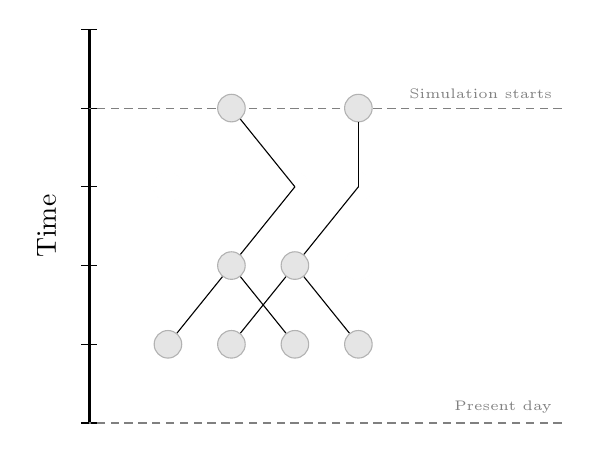
\begin{tikzpicture}[node distance=5mm and 5mm]

\tikzset{greynode/.style={font=\footnotesize,node distance=1cm and 1 cm,fill=black!10,draw=black!30,inner sep=0pt,minimum size=3.5mm,shape=circle},
whitenode/.style={font=\footnotesize,node distance=1cm and 1 cm,fill=white,draw=white,inner sep=0pt,minimum size=3.7mm,shape=circle},
mutations/.style={shape=starburst,fill=red!50!blue,inner sep=0.8pt,starburst points=11,starburst point height=.2cm}}

\node (timestart) at (0,-4) {};

% Axis
\node (leftAx) at ($(-1,0) + (timestart)$) {};
\draw[very thick] ($(-1,0) + (timestart)$) -- +(0, 5);
\foreach \y in {0, 1, 2, 3, 4, 5} \draw ($(leftAx) + (-0.1, \y)$) -- ($(leftAx) + (0.1, \y)$); % tick marks
%\node[anchor=east] at ($(leftAx)$) {0}; \node[anchor=east] at ($(leftAx) + (0,5)$) {5};
\node[rotate=90,anchor=south] (leftLabel) at ($(leftAx) + (-0.3,2.5)$) {$\textrm{Time}$};

% Time arrow
\draw[densely dashed,color=gray] ($(5,0) + (timestart)$) node[above left] {\tiny Present day} -- ($(-1,0) + (timestart)$);
\draw[densely dashed,color=gray] ($(5,4) + (timestart)$) node[above left] {\tiny Simulation starts} -- ($(-1,4) + (timestart)$);

% sample nodes
\node (s1) {};
\node (s2) [right=of s1,greynode] {};
\node (s3) [right=of s2] {};
\node (s4) [right=of s3,greynode] {};

% Non-sample nodes
\foreach \x in {1,2,3,4} \foreach \y in {1,2,3} \node[greynode] (s\x\y) at ($(s\x) + (0,-\y)$) {};

% Remove some nodes
\node[whitenode] at (s21) {};
\foreach \y in {1,2} \node[whitenode] at (s1\y) {};
\node[whitenode] at (s42){}; \node[whitenode] at (s12){};
\node[whitenode] at (s31){}; \node[whitenode] at (s41){};

% Edges 
\draw (s2) -- (s31.center); \draw (s4) -- (s41.center);
\draw (s22) -- (s31.center); \draw (s41.center) -- (s32);
\draw (s13) -- (s22) -- (s33); \draw (s23) -- (s32) -- (s43);

\end{tikzpicture} 

\end{minipage}\hfill
\begin{minipage}{.4\textwidth}
Alternates between
\begin{enumerate}
\item forward simulation
\item pruning of irrelevant history.
\end{enumerate}
\end{minipage}
\end{frame}

%\begin{frame}
%\frametitle{\texttt{SLiM} simulates \magenta{an entire population} forward-in-time}
%\begin{minipage}{.58\textwidth}
%
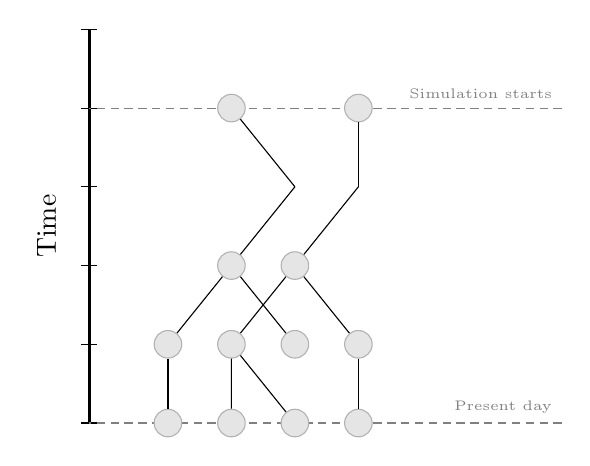
\begin{tikzpicture}[node distance=5mm and 5mm]

\tikzset{greynode/.style={font=\footnotesize,node distance=1cm and 1 cm,fill=black!10,draw=black!30,inner sep=0pt,minimum size=3.5mm,shape=circle},
whitenode/.style={font=\footnotesize,node distance=1cm and 1 cm,fill=white,draw=white,inner sep=0pt,minimum size=3.7mm,shape=circle},
mutations/.style={shape=starburst,fill=red!50!blue,inner sep=0.8pt,starburst points=11,starburst point height=.2cm}}

\node (timestart) at (0,-4) {};

% Axis
\node (leftAx) at ($(-1,0) + (timestart)$) {};
\draw[very thick] ($(-1,0) + (timestart)$) -- +(0, 5);
\foreach \y in {0, 1, 2, 3, 4, 5} \draw ($(leftAx) + (-0.1, \y)$) -- ($(leftAx) + (0.1, \y)$); % tick marks
%\node[anchor=east] at ($(leftAx)$) {0}; \node[anchor=east] at ($(leftAx) + (0,5)$) {5};
\node[rotate=90,anchor=south] (leftLabel) at ($(leftAx) + (-0.3,2.5)$) {$\textrm{Time}$};

% Time arrow
\draw[densely dashed,color=gray] ($(5,0) + (timestart)$) node[above left] {\tiny Present day} -- ($(-1,0) + (timestart)$);
\draw[densely dashed,color=gray] ($(5,4) + (timestart)$) node[above left] {\tiny Simulation starts} -- ($(-1,4) + (timestart)$);

% sample nodes
\node (s1) [] {};
\node (s2) [right=of s1,greynode] {};
\node (s3) [right=of s2] {};
\node (s4) [right=of s3,greynode] {};

% Non-sample nodes
\foreach \x in {1,2,3,4} \foreach \y in {1,2,3,4} \node[greynode] (s\x\y) at ($(s\x) + (0,-\y)$) {};

% Remove some nodes
\node[whitenode] at (s21) {}; \node[whitenode] at (s11) {}; \node[whitenode] at (s41){};
\node[whitenode] at (s31) {}; \node[whitenode] at (s42) {}; \node[whitenode] at (s12){};

% Edges 
 \draw (s2) -- (s31.center); \draw (s4) -- (s41.center);
\draw (s22) -- (s31.center); \draw (s41.center) -- (s32);
\draw (s13) -- (s22) -- (s33); \draw (s23) -- (s32) -- (s43);
\draw (s14) -- (s13); \draw (s24) -- (s23) -- (s34); \draw (s43) -- (s44);

\end{tikzpicture} 

%\end{minipage}\hfill
%\begin{minipage}{.4\textwidth}
%Alternates between
%\begin{enumerate}
%\item \magenta{forward simulation}
%\item pruning of irrelevant history.
%\end{enumerate}
%\end{minipage}
%\end{frame}

\begin{frame}
\frametitle{\texttt{SLiM} simulates \magenta{an entire population} forward-in-time}
\begin{minipage}{.58\textwidth}

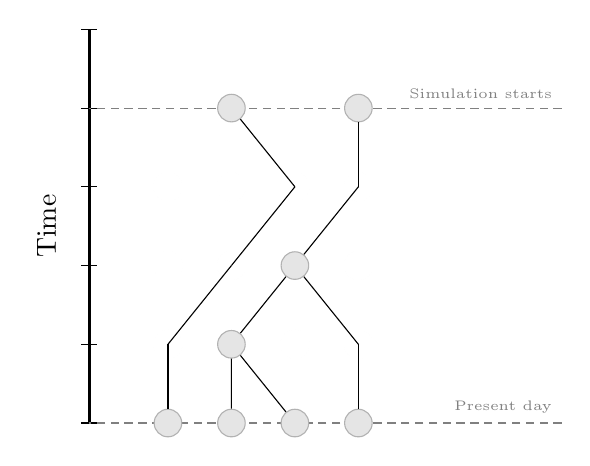
\begin{tikzpicture}[node distance=5mm and 5mm]

\tikzset{greynode/.style={font=\footnotesize,node distance=1cm and 1 cm,fill=black!10,draw=black!30,inner sep=0pt,minimum size=3.5mm,shape=circle},
whitenode/.style={font=\footnotesize,node distance=1cm and 1 cm,fill=white,draw=white,inner sep=0pt,minimum size=3.7mm,shape=circle},
mutations/.style={shape=starburst,fill=red!50!blue,inner sep=0.8pt,starburst points=11,starburst point height=.2cm}}

\node (timestart) at (0,-4) {};

% Axis
\node (leftAx) at ($(-1,0) + (timestart)$) {};
\draw[very thick] ($(-1,0) + (timestart)$) -- +(0, 5);
\foreach \y in {0, 1, 2, 3, 4, 5} \draw ($(leftAx) + (-0.1, \y)$) -- ($(leftAx) + (0.1, \y)$); % tick marks
%\node[anchor=east] at ($(leftAx)$) {0}; \node[anchor=east] at ($(leftAx) + (0,5)$) {5};
\node[rotate=90,anchor=south] (leftLabel) at ($(leftAx) + (-0.3,2.5)$) {$\textrm{Time}$};

% Time arrow
\draw[densely dashed,color=gray] ($(5,0) + (timestart)$) node[above left] {\tiny Present day} -- ($(-1,0) + (timestart)$);
\draw[densely dashed,color=gray] ($(5,4) + (timestart)$) node[above left] {\tiny Simulation starts} -- ($(-1,4) + (timestart)$);

% sample nodes
\node (s1) [] {};
\node (s2) [right=of s1,greynode] {};
\node (s3) [right=of s2] {};
\node (s4) [right=of s3,greynode] {};

% Non-sample nodes
\foreach \x in {1,2,3,4} \foreach \y in {1,2,3,4} \node[greynode] (s\x\y) at ($(s\x) + (0,-\y)$) {};

% Remove some nodes
\node[whitenode] at (s21) {}; \node[whitenode] at (s11) {}; \node[whitenode] at (s41){};
\node[whitenode] at (s31) {}; \node[whitenode] at (s42) {}; \node[whitenode] at (s12){};
\node[whitenode] at (s33){}; \node[whitenode] at (s13){}; \node[whitenode] at (s43){};
\node[whitenode] at (s22){};

% Edges 
 \draw (s2) -- (s31.center); \draw (s4) -- (s41.center);
\draw (s22.center) -- (s31.center); \draw (s41.center) -- (s32);
\draw (s13.center) -- (s22.center); \draw (s23) -- (s32) -- (s43.center);
\draw (s14) -- (s13.center); \draw (s24) -- (s23) -- (s34); \draw (s43.center) -- (s44);

\end{tikzpicture} 

\end{minipage}\hfill
\begin{minipage}{.4\textwidth}
Alternates between
\begin{enumerate}
\item forward simulation
\item pruning of irrelevant history.
\end{enumerate}
\end{minipage}
\end{frame}

%\begin{frame}
%\frametitle{\texttt{SLiM} simulates \magenta{an entire population} forward-in-time}
%\begin{minipage}{.58\textwidth}
%
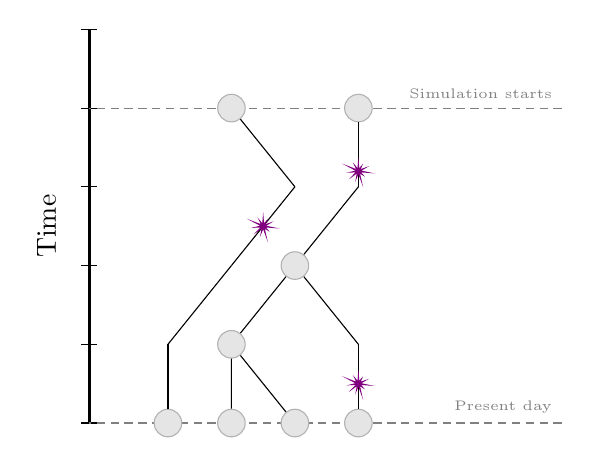
\begin{tikzpicture}[node distance=5mm and 5mm]

\tikzset{greynode/.style={font=\footnotesize,node distance=1cm and 1 cm,fill=black!10,draw=black!30,inner sep=0pt,minimum size=3.5mm,shape=circle},
whitenode/.style={font=\footnotesize,node distance=1cm and 1 cm,fill=white,draw=white,inner sep=0pt,minimum size=3.7mm,shape=circle},
mutations/.style={shape=starburst,fill=red!50!blue,inner sep=0.8pt,starburst points=11,starburst point height=.2cm}}

\node (timestart) at (0,-4) {};

% Axis
\node (leftAx) at ($(-1,0) + (timestart)$) {};
\draw[very thick] ($(-1,0) + (timestart)$) -- +(0, 5);
\foreach \y in {0, 1, 2, 3, 4, 5} \draw ($(leftAx) + (-0.1, \y)$) -- ($(leftAx) + (0.1, \y)$); % tick marks
%\node[anchor=east] at ($(leftAx)$) {0}; \node[anchor=east] at ($(leftAx) + (0,5)$) {5};
\node[rotate=90,anchor=south] (leftLabel) at ($(leftAx) + (-0.3,2.5)$) {$\textrm{Time}$};

% Time arrow
\draw[densely dashed,color=gray] ($(5,0) + (timestart)$) node[above left] {\tiny Present day} -- ($(-1,0) + (timestart)$);
\draw[densely dashed,color=gray] ($(5,4) + (timestart)$) node[above left] {\tiny Simulation starts} -- ($(-1,4) + (timestart)$);

% sample nodes
\node (s1) [] {};
\node (s2) [right=of s1,greynode] {};
\node (s3) [right=of s2] {};
\node (s4) [right=of s3,greynode] {};

% Non-sample nodes
\foreach \x in {1,2,3,4} \foreach \y in {1,2,3,4} \node[greynode] (s\x\y) at ($(s\x) + (0,-\y)$) {};

% Remove some nodes
\node[whitenode] at (s21) {}; \node[whitenode] at (s11) {}; \node[whitenode] at (s41){};
\node[whitenode] at (s31) {}; \node[whitenode] at (s42) {}; \node[whitenode] at (s12){};
\node[whitenode] at (s33){}; \node[whitenode] at (s13){}; \node[whitenode] at (s43){};
\node[whitenode] at (s22){};

% Edges 
 \draw (s2) -- (s31.center); \draw (s4) -- (s41.center);
\draw (s22.center) -- (s31.center); \draw (s41.center) -- (s32);
\draw (s13.center) -- (s22.center); \draw (s23) -- (s32) -- (s43.center);
\draw (s14) -- (s13.center); \draw (s24) -- (s23) -- (s34); \draw (s43.center) -- (s44);

% Mutations
\node[mutations] at ($(s22)!.5!(s31)$){};
\node[mutations] at ($(s4)!.8!(s41)$){};
\node[mutations] at ($(s43)!.5!(s44)$){};

\end{tikzpicture} 

%\end{minipage}\hfill
%\begin{minipage}{.4\textwidth}
%Mutations can be added during the simulation of the tree topologies, or generated independently and added afterwards.
%\end{minipage}
%\end{frame}

\begin{frame}
\frametitle{\texttt{SLiM} performance}
\begin{center}
\small
\centering
\setlength{\aboverulesep}{5pt}
\setlength{\belowrulesep}{5pt}
\begin{tabularx}{.9\textwidth}{p{2cm}p{2cm}p{1.9cm}p{1.9cm}X}
\toprule
%& \multicolumn{3}{c}{{\bf Global ancestry}} \\[1mm]
 & Missing data & Run time & File size & Realism \\
\midrule 
%{\bf default} & $4.0$\% & 6 sec &  9 Mb & \crossmark \\ \addlinespace
\texttt{msprime}& $0.0$\% & 53 sec  &  1700 Mb & \crossmark \\ \addlinespace
\magenta{\texttt{SLiM}} & \magenta{$0.0$\%} & \magenta{$>1$ hr} & \magenta{41 Mb} & \magenta{\checkmark}  \\
\bottomrule
\end{tabularx}
\end{center}
\vspace{5mm}
\end{frame}

\section{Simulating tree sequences: new method}

\begin{frame}
\begin{center}
\centering

\begin{tikzpicture}[node distance=2mm and 2mm,xscale=.8,yscale=.6,font=\tiny]

\tikzset{greynode/.style={font=\footnotesize,node distance=1cm and 1 cm,fill=black!10,draw=black!30,inner sep=0pt,minimum size=3mm,shape=circle},
rednode/.style={font=\footnotesize,node distance=1cm and 1 cm,fill=red!30,draw=red!50,inner sep=0pt,minimum size=3mm,shape=circle},
bluenode/.style={font=\footnotesize,node distance=1cm and 1 cm,fill=blue!30,draw=blue!50,inner sep=0pt,minimum size=3mm,shape=circle},
purplenode/.style={font=\footnotesize,node distance=1cm and 1cm,fill=purple!30,draw=purple!50,inner sep=0pt,minimum size=3mm,shape=circle},
whitenode/.style={font=\footnotesize,node distance=1cm and 1cm,fill=white,draw=white,inner sep=0pt,minimum size=3.3mm,shape=circle}}

% Axis
\node (leftAx) at (-6,0) {};
\draw[very thick] (-6,0) -- +(0, 10);
\foreach \y in {0, 1, 2, 3, 4, 5, 6, 7, 8, 9, 10} \draw ($(leftAx) + (-0.1, \y)$) -- ($(leftAx) + (0.1, \y)$); % tick marks
\node[rotate=90,anchor=south] (leftLabel) at ($(leftAx) + (-0.3,5)$) {$\footnotesize\textrm{Time}$};

% Important times
\draw[gray,densely dashed] ($(leftAx) + (0,4)$) -- +(16, 0);

% Sample nodes
\node(s1) [purplenode] at (0,0) {};
\node (s2) [purplenode,right of=s1] {};
\node (s3) [purplenode,right of=s2] {};
\node (s4) [purplenode,right of=s3] {};
%
%% Other purple nodes
%
%\foreach \x in {1,2,3,4} \foreach \y in {1,2,3} \node[purplenode] (u\x\y) at ($(s\x) + (0, \y)$) {};

% Ancestral nodes
\node (pop1) at (-5, 4) {};
\node (pop2) at (5, 4) {};
\foreach \x in {1,2,3,4} \node[bluenode] (b\x) at ($(pop1) + (s\x)$) {};
\foreach \x in {1,2,3,4} \node[rednode] (r\x) at ($(pop2) + (s\x)$) {};

% SLiM-simulated edges
%\draw (s1) -- (u11) -- (u32) -- (u43) -- (r2);
%\draw (s2) -- (u21) -- (u12) -- (u23) -- (b3);
%\draw (s3) -- (u31) -- (u22) -- (u13) -- (b2);
%\draw (s4) -- (u41) -- (u32) -- (u43);
%\draw (u42) -- (u33) -- (r1);

% Population labels
\node at ($0.5*(s2) + 0.5*(s3) + (0,-0.5)$) {$\tiny\textrm{Admixed population}$};
\node at ($(pop1) + 0.5*(s2) + 0.5*(s3) + (0,+0.5)$) {$\tiny\textrm{Blue ancestors}$};
\node at ($(pop2) + 0.5*(s2) + 0.5*(s3) + (0,+0.5)$) {$\tiny\textrm{Red ancestors}$};

% Cover the bottom bit
\foreach \x in {1,2,3,4} \node[whitenode] at (s\x) {};

% Time of admixture
\node[anchor=south,color=gray] at ($0.5*(b4) + 0.5*(r1)$) {{\tiny Start of admixture}};

\end{tikzpicture} 

\end{center}
\end{frame}

\begin{frame}
\begin{center}
\centering

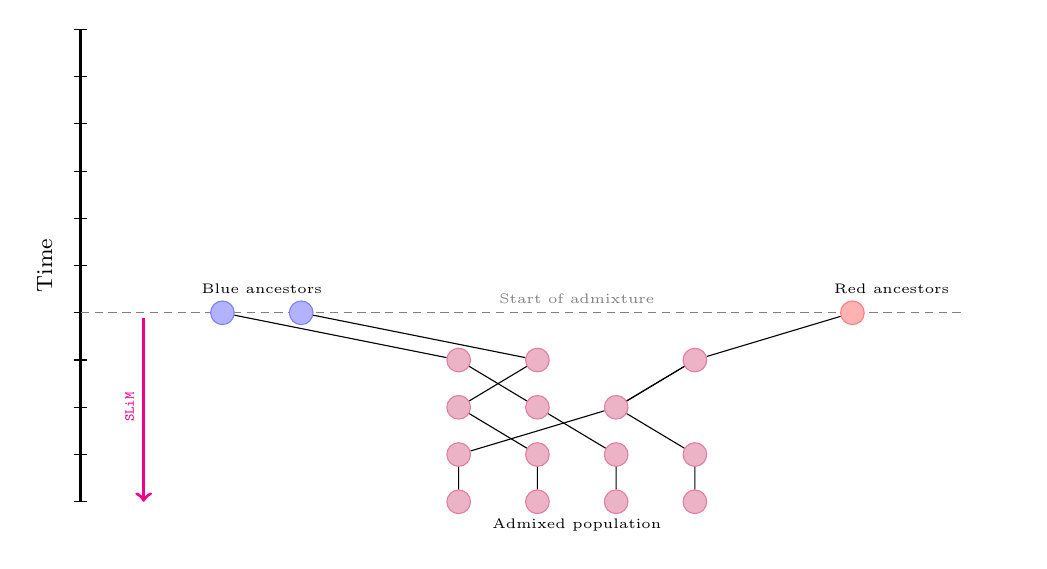
\begin{tikzpicture}[node distance=2mm and 2mm,xscale=.8,yscale=.6,font=\tiny]

\tikzset{greynode/.style={font=\footnotesize,node distance=1cm and 1 cm,fill=black!10,draw=black!30,inner sep=0pt,minimum size=3mm,shape=circle},
rednode/.style={font=\footnotesize,node distance=1cm and 1 cm,fill=red!30,draw=red!50,inner sep=0pt,minimum size=3mm,shape=circle},
bluenode/.style={font=\footnotesize,node distance=1cm and 1 cm,fill=blue!30,draw=blue!50,inner sep=0pt,minimum size=3mm,shape=circle},
purplenode/.style={font=\footnotesize,node distance=1cm and 1cm,fill=purple!30,draw=purple!50,inner sep=0pt,minimum size=3mm,shape=circle},
whitenode/.style={font=\footnotesize,node distance=1cm and 1cm,fill=white,draw=white,inner sep=0pt,minimum size=3.3mm,shape=circle}}

% Axis
\node (leftAx) at (-6,0) {};
\draw[very thick] (-6,0) -- +(0, 10);
\foreach \y in {0, 1, 2, 3, 4, 5, 6, 7, 8, 9, 10} \draw ($(leftAx) + (-0.1, \y)$) -- ($(leftAx) + (0.1, \y)$); % tick marks
\node[rotate=90,anchor=south] (leftLabel) at ($(leftAx) + (-0.3,5)$) {\footnotesize$\textrm{Time}$};

% Important times
\draw[gray,densely dashed] ($(leftAx) + (0,4)$) -- +(14, 0);

% Sample nodes
\node[purplenode] (s1) at (0,0) {};
\node (s2) [purplenode,right of=s1] {};
\node (s3) [purplenode,right of=s2] {};
\node (s4) [purplenode,right of=s3] {};
%
%% Other purple nodes
%
\foreach \x in {1,2,3,4} \foreach \y in {1,2,3} \node[purplenode] (u\x\y) at ($(s\x) + (0, \y)$) {};

% Ancestral nodes
\node (pop1) at (-5, 4) {};
\node (pop2) at (5, 4) {};
\foreach \x in {2,3} \node[bluenode] (b\x) at ($(pop1) + (s\x)$) {};
\foreach \x in {1,4} \node (b\x) at ($(pop1) + (s\x)$) {};
\foreach \x in {1,3,4} \node (r\x) at ($(pop2) + (s\x)$) {};
\node[rednode] (r2) at ($(pop2) + (s2)$) {};

% SLiM-simulated edges
\draw (s1) -- (u11) -- (u32) -- (u43) -- (r2);
\draw (s2) -- (u21) -- (u12) -- (u23) -- (b3);
\draw (s3) -- (u31) -- (u22) -- (u13) -- (b2);
\draw (s4) -- (u41) -- (u32) -- (u43);

% Population labels
\node at ($0.5*(s2) + 0.5*(s3) + (0,-0.5)$) {$\tiny\textrm{Admixed population}$};
\node at ($(pop1) + 0.5*(s2) + 0.5*(s3) + (0,+0.5)$) {$\tiny\textrm{Blue ancestors}$};
\node at ($(pop2) + 0.5*(s2) + 0.5*(s3) + (0,+0.5)$) {$\tiny\textrm{Red ancestors}$};

% white nodes
\node[whitenode] at (u42){}; \node[whitenode] at (u33){};

% simulation label
\draw[very thick,<-,magenta] ($(s1) + (-5,0)$) -- +(0,3.9);
\node[rotate=90,anchor=south,magenta] (SLiM) at ($(s1) + (-5,0) + (0,2)$) {$\texttt{SLiM}$};

% Time of admixture
\node[anchor=south,color=gray] at ($0.5*(b4) + 0.5*(r1)$) {{\tiny Start of admixture}};

\end{tikzpicture} 

\end{center}
\end{frame}

\begin{frame}
\begin{center}
\centering

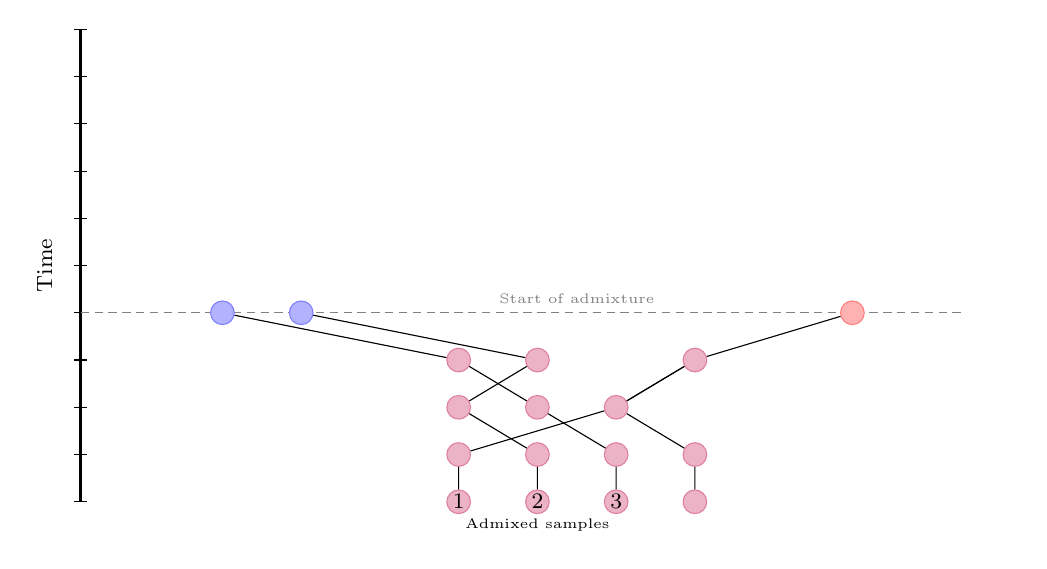
\begin{tikzpicture}[node distance=2mm and 2mm,xscale=.8,yscale=.6,font=\tiny]

\tikzset{greynode/.style={font=\footnotesize,node distance=1cm and 1 cm,fill=black!10,draw=black!30,inner sep=0pt,minimum size=3mm,shape=circle},
rednode/.style={font=\footnotesize,node distance=1cm and 1 cm,fill=red!30,draw=red!50,inner sep=0pt,minimum size=3mm,shape=circle},
bluenode/.style={font=\footnotesize,node distance=1cm and 1 cm,fill=blue!30,draw=blue!50,inner sep=0pt,minimum size=3mm,shape=circle},
purplenode/.style={font=\footnotesize,node distance=1cm and 1cm,fill=purple!30,draw=purple!50,inner sep=0pt,minimum size=3mm,shape=circle},
whitenode/.style={font=\footnotesize,node distance=1cm and 1cm,fill=white,draw=white,inner sep=0pt,minimum size=3.3mm,shape=circle}}

% Axis
\node (leftAx) at (-6,0) {};
\draw[very thick] (-6,0) -- +(0, 10);
\foreach \y in {0, 1, 2, 3, 4, 5, 6, 7, 8, 9, 10} \draw ($(leftAx) + (-0.1, \y)$) -- ($(leftAx) + (0.1, \y)$); % tick marks
\node[rotate=90,anchor=south] (leftLabel) at ($(leftAx) + (-0.3,5)$) {\footnotesize$\textrm{Time}$};

% Important times
\draw[gray,densely dashed] ($(leftAx) + (0,4)$) -- +(14, 0);

% Sample nodes
\node[purplenode] (s1) at (0,0) {1};
\node (s2) [purplenode,right of=s1] {2};
\node (s3) [purplenode,right of=s2] {3};
\node (s4) [purplenode,right of=s3] {};
%
%% Other purple nodes
%
\foreach \x in {1,2,3,4} \foreach \y in {1,2,3} \node[purplenode] (u\x\y) at ($(s\x) + (0, \y)$) {};

% Ancestral nodes
\node (pop1) at (-5, 4) {};
\node (pop2) at (5, 4) {};
\foreach \x in {2,3} \node[bluenode] (b\x) at ($(pop1) + (s\x)$) {};
\foreach \x in {1,4} \node (b\x) at ($(pop1) + (s\x)$) {};
\foreach \x in {1,3,4} \node (r\x) at ($(pop2) + (s\x)$) {};
\node[rednode] (r2) at ($(pop2) + (s2)$) {};

% SLiM-simulated edges
\draw (s1) -- (u11) -- (u32) -- (u43) -- (r2);
\draw (s2) -- (u21) -- (u12) -- (u23) -- (b3);
\draw (s3) -- (u31) -- (u22) -- (u13) -- (b2);
\draw (s4) -- (u41) -- (u32) -- (u43);

% Population labels
%\node at ($0.5*(s1) + 0.5*(s3) + (0,-0.5)$) {$\tiny\textrm{Admixed samples}$};

% white nodes
\node[whitenode] at (u42){}; \node[whitenode] at (u33){};

% samples
%\draw[red,very thick] ($(s1.north)+(-.3,.3)$) -- ($(s3.north) + (.3,.3)$) -- ($(s3.south) + (.3,-.3)$) -- ($(s1.south)+(-.3,-.3)$)-- cycle;

% Time of admixture
\node[anchor=south,color=gray] at ($0.5*(b4) + 0.5*(r1)$) {{\tiny Start of admixture}};

% Population labels
\node at ($0.5*(s1) + 0.5*(s3) + (0,-0.5)$) {$\tiny\textrm{Admixed samples}$};

\end{tikzpicture} 

\end{center}
\end{frame}

\begin{frame}
\begin{center}
\centering

\begin{tikzpicture}[node distance=2mm and 2mm,xscale=.8,yscale=.6,font=\tiny]

\tikzset{greynode/.style={font=\footnotesize,node distance=1cm and 1 cm,fill=black!10,draw=black!30,inner sep=0pt,minimum size=3mm,shape=circle},
rednode/.style={font=\footnotesize,node distance=1cm and 1 cm,fill=red!30,draw=red!50,inner sep=0pt,minimum size=3mm,shape=circle},
bluenode/.style={font=\footnotesize,node distance=1cm and 1 cm,fill=blue!30,draw=blue!50,inner sep=0pt,minimum size=3mm,shape=circle},
purplenode/.style={font=\footnotesize,node distance=1cm and 1cm,fill=purple!30,draw=purple!50,inner sep=0pt,minimum size=3mm,shape=circle},
whitenode/.style={font=\footnotesize,node distance=1cm and 1cm,fill=white,draw=white,inner sep=0pt,minimum size=3.3mm,shape=circle}}

% Axis
\node (leftAx) at (-6,0) {};
\draw[very thick] (-6,0) -- +(0, 10);
\foreach \y in {0, 1, 2, 3, 4, 5, 6, 7, 8, 9, 10} \draw ($(leftAx) + (-0.1, \y)$) -- ($(leftAx) + (0.1, \y)$); % tick marks
\node[rotate=90,anchor=south] (leftLabel) at ($(leftAx) + (-0.3,5)$) {$\footnotesize\textrm{Time}$};

% Important times
\draw[gray,densely dashed] ($(leftAx) + (0,4)$) -- +(14, 0);

% Sample nodes
\node[purplenode] (s1) at (0,0) {1};
\node (s2) [purplenode,right of=s1] {2};
\node (s3) [purplenode,right of=s2] {3};
\node (s4) [purplenode,right of=s3] {};
%
%% Other purple nodes
%
\foreach \x in {1,2,3,4} \foreach \y in {1,2,3} \node[purplenode] (u\x\y) at ($(s\x) + (0, \y)$) {};

% Ancestral nodes
\node (pop1) at (-5, 4) {};
\node (pop2) at (5, 4) {};
\foreach \x in {2,3} \node[bluenode] (b\x) at ($(pop1) + (s\x)$) {};
\foreach \x in {1,4} \node (b\x) at ($(pop1) + (s\x)$) {};
\foreach \x in {1,3,4} \node (r\x) at ($(pop2) + (s\x)$) {};
\node[rednode] (r2) at ($(pop2) + (s2)$) {};

% Population labels
\node at ($0.5*(s1) + 0.5*(s3) + (0,-0.5)$) {$\tiny\textrm{Admixed samples}$};

% Population labels
%\node at ($0.5*(s1) + 0.5*(s3) + (0,-0.5)$) {$\tiny\textrm{Admixed samples}$};

% white nodes
\node[whitenode] at (u42){}; \node[whitenode] at (u33){};
\node[whitenode] at (s4){}; \node[whitenode] at (u41){};
\foreach \x in {1,2,3,4} \foreach \y in {1,2,3} \node[whitenode] (u\x\y) at ($(s\x) + (0, \y)$) {};

% samples
%\draw[red,very thick] ($(s1.north)+(-.3,.3)$) -- ($(s3.north) + (.3,.3)$) -- ($(s3.south) + (.3,-.3)$) -- ($(s1.south)+(-.3,-.3)$)-- cycle;

% Time of admixture
\node[anchor=south,color=gray] at ($0.5*(b4) + 0.5*(r1)$) {{\tiny Start of admixture}};

% SLiM-simulated edges
\draw (s1) -- (u11.center) -- (u32.center) -- (u43.center) -- (r2);
\draw (s2) -- (u21.center) -- (u12.center) -- (u23.center) -- (b3);
\draw (s3) -- (u31.center) -- (u22.center) -- (u13.center) -- (b2);
\draw (u32.center) -- (u43.center);

\end{tikzpicture} 

\end{center}
\end{frame}

\begin{frame}
\begin{center}
\centering

\begin{tikzpicture}[node distance=2mm and 2mm,xscale=.8,yscale=.6,font=\tiny]

\tikzset{greynode/.style={font=\footnotesize,node distance=1cm and 1 cm,fill=black!10,draw=black!30,inner sep=0pt,minimum size=3mm,shape=circle},
rednode/.style={font=\footnotesize,node distance=1cm and 1 cm,fill=red!30,draw=red!50,inner sep=0pt,minimum size=3mm,shape=circle},
bluenode/.style={font=\footnotesize,node distance=1cm and 1 cm,fill=blue!30,draw=blue!50,inner sep=0pt,minimum size=3mm,shape=circle},
purplenode/.style={font=\footnotesize,node distance=1cm and 1cm,fill=purple!30,draw=purple!50,inner sep=0pt,minimum size=3mm,shape=circle},
whitenode/.style={font=\footnotesize,node distance=1cm and 1cm,fill=white,draw=white,inner sep=0pt,minimum size=3.3mm,shape=circle},
mutations/.style={shape=starburst,fill=red!50!blue,inner sep=0.8pt,starburst points=11,starburst point height=.2cm}}

% Axis
\node (leftAx) at (-6,0) {};
\draw[very thick] (-6,0) -- +(0, 10);
\foreach \y in {0, 1, 2, 3, 4, 5, 6, 7, 8, 9, 10} \draw ($(leftAx) + (-0.1, \y)$) -- ($(leftAx) + (0.1, \y)$); % tick marks
\node[rotate=90,anchor=south] (leftLabel) at ($(leftAx) + (-0.3,5)$) {$\footnotesize\textrm{Time}$};

% Important times
\draw[gray,densely dashed] ($(leftAx) + (0,4)$) -- +(14, 0);

% Sample nodes
\node[purplenode] (s1) at (0,0) {1};
\node (s2) [purplenode,right of=s1] {2};
\node (s3) [purplenode,right of=s2] {3};
\node (s4) [purplenode,right of=s3] {};
%
%% Other purple nodes
%
\foreach \x in {1,2,3,4} \foreach \y in {1,2,3} \node[purplenode] (u\x\y) at ($(s\x) + (0, \y)$) {};

% Ancestral nodes
\node (pop1) at (-5, 4) {};
\node (pop2) at (5, 4) {};
\foreach \x in {2,3} \node[bluenode] (b\x) at ($(pop1) + (s\x)$) {};
\foreach \x in {1,4} \node (b\x) at ($(pop1) + (s\x)$) {};
\foreach \x in {1,3,4} \node (r\x) at ($(pop2) + (s\x)$) {};
\node[rednode] (r2) at ($(pop2) + (s2)$) {};

% Population labels
\node at ($0.5*(s1) + 0.5*(s3) + (0,-0.5)$) {$\tiny\textrm{Admixed samples}$};

% Population labels
%\node at ($0.5*(s1) + 0.5*(s3) + (0,-0.5)$) {$\tiny\textrm{Admixed samples}$};

% white nodes
\node[whitenode] at (u42){}; \node[whitenode] at (u33){};
\node[whitenode] at (s4){}; \node[whitenode] at (u41){};
\foreach \x in {1,2,3,4} \foreach \y in {1,2,3} \node[whitenode] (u\x\y) at ($(s\x) + (0, \y)$) {};

% samples
%\draw[red,very thick] ($(s1.north)+(-.3,.3)$) -- ($(s3.north) + (.3,.3)$) -- ($(s3.south) + (.3,-.3)$) -- ($(s1.south)+(-.3,-.3)$)-- cycle;

% Time of admixture
\node[anchor=south,color=gray] at ($0.5*(b4) + 0.5*(r1)$) {{\tiny Start of admixture}};

% SLiM-simulated edges
\draw (s1) -- (u11.center) -- (u32.center) -- (u43.center) -- (r2);
\draw (s2) -- (u21.center) -- (u12.center) -- (u23.center) -- (b3);
\draw (s3) -- (u31.center) -- (u22.center) -- (u13.center) -- (b2);
\draw (u32.center) -- (u43.center);

% Mutations
\node[mutations] at ($(u11)!.5!(u32)$) {};
\node[mutations] at ($(u13)!.7!(u22)$) {};

\end{tikzpicture} 

\end{center}
\end{frame}

\begin{frame}
\begin{center}
\centering

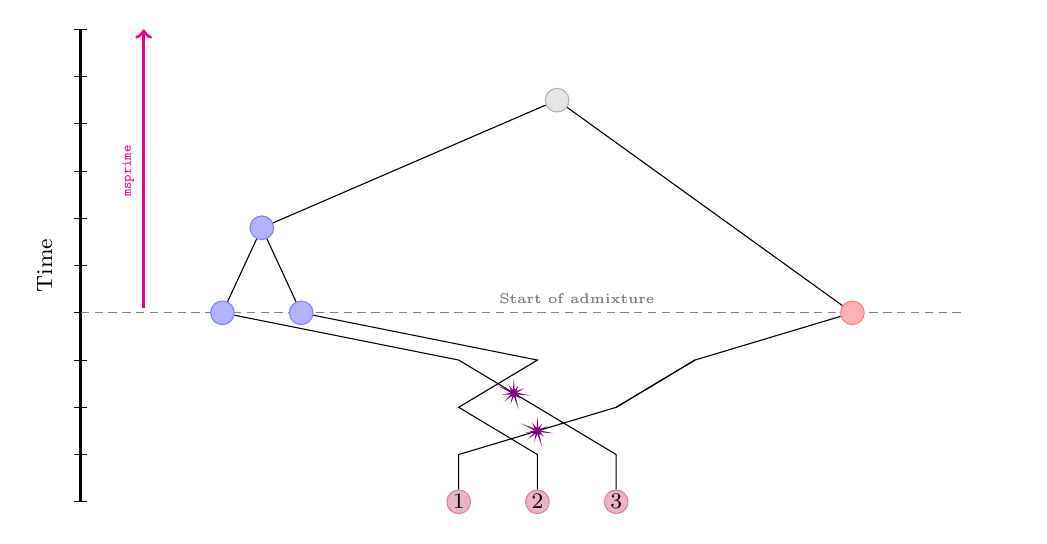
\begin{tikzpicture}[node distance=2mm and 2mm,xscale=.8,yscale=.6,font=\tiny]

\tikzset{greynode/.style={font=\footnotesize,node distance=1cm and 1 cm,fill=black!10,draw=black!30,inner sep=0pt,minimum size=3mm,shape=circle},
rednode/.style={font=\footnotesize,node distance=1cm and 1 cm,fill=red!30,draw=red!50,inner sep=0pt,minimum size=3mm,shape=circle},
bluenode/.style={font=\footnotesize,node distance=1cm and 1 cm,fill=blue!30,draw=blue!50,inner sep=0pt,minimum size=3mm,shape=circle},
purplenode/.style={font=\footnotesize,node distance=1cm and 1cm,fill=purple!30,draw=purple!50,inner sep=0pt,minimum size=3mm,shape=circle},
whitenode/.style={font=\footnotesize,node distance=1cm and 1cm,fill=white,draw=white,inner sep=0pt,minimum size=3.3mm,shape=circle},
mutations/.style={shape=starburst,fill=red!50!blue,inner sep=0.8pt,starburst points=11,starburst point height=.2cm}}

% Axis
\node (leftAx) at (-6,0) {};
\draw[very thick] (-6,0) -- +(0, 10);
\foreach \y in {0, 1, 2, 3, 4, 5, 6, 7, 8, 9, 10} \draw ($(leftAx) + (-0.1, \y)$) -- ($(leftAx) + (0.1, \y)$); % tick marks
\node[rotate=90,anchor=south] (leftLabel) at ($(leftAx) + (-0.3,5)$) {$\footnotesize\textrm{Time}$};

% Important times
\draw[gray,densely dashed] ($(leftAx) + (0,4)$) -- +(14, 0);

% Sample nodes
\node[purplenode] (s1) at (0,0) {1};
\node (s2) [purplenode,right of=s1] {2};
\node (s3) [purplenode,right of=s2] {3};
\node (s4) [purplenode,right of=s3] {};
%
%% Other purple nodes
%
\foreach \x in {1,2,3,4} \foreach \y in {1,2,3} \node[purplenode] (u\x\y) at ($(s\x) + (0, \y)$) {};

% Ancestral nodes
\node (pop1) at (-5, 4) {};
\node (pop2) at (5, 4) {};
\foreach \x in {2,3} \node[bluenode] (b\x) at ($(pop1) + (s\x)$) {};
\foreach \x in {1,4} \node (b\x) at ($(pop1) + (s\x)$) {};
\foreach \x in {1,3,4} \node (r\x) at ($(pop2) + (s\x)$) {};
\node[rednode] (r2) at ($(pop2) + (s2)$) {};

% white nodes
\node[whitenode] at (u42){}; \node[whitenode] at (u33){};
\node[whitenode] at (s4){}; \node[whitenode] at (u41){};
\foreach \x in {1,2,3,4} \foreach \y in {1,2,3} \node[whitenode] (u\x\y) at ($(s\x) + (0, \y)$) {};

% samples
%\draw[red,very thick] ($(s1.north)+(-.3,.3)$) -- ($(s3.north) + (.3,.3)$) -- ($(s3.south) + (.3,-.3)$) -- ($(s1.south)+(-.3,-.3)$)-- cycle;

% Time of admixture
\node[anchor=south,color=gray] at ($0.5*(b4) + 0.5*(r1)$) {{\tiny Start of admixture}};

% SLiM-simulated edges
\draw (s1) -- (u11.center) -- (u32.center) -- (u43.center) -- (r2);
\draw (s2) -- (u21.center) -- (u12.center) -- (u23.center) -- (b3);
\draw (s3) -- (u31.center) -- (u22.center) -- (u13.center) -- (b2);
\draw (u32.center) -- (u43.center);

% Mutations
\node[mutations] at ($(u11)!.5!(u32)$) {};
\node[mutations] at ($(u13)!.7!(u22)$) {};

% msprime nodes
\node[bluenode] (b5) at ($0.5*(b2)+0.5*(b3)+(0,1.8)$) {}; 
\node[greynode] (g1) at ($0.5*(b5)+0.5*(r2)+(0,3.6)$) {};

% msprime edges
\draw (b2) -- (b5) -- (b3); \draw (b5) -- (g1) -- (r2);

% simulation label
\draw[very thick,->,magenta] ($(b1) + (0,0.1)$) -- +(0,5.9);
\node[rotate=90,anchor=south,magenta] (msprime) at ($(b1) + (0,3)$) {$\texttt{msprime}$};

% Time of admixture
\node[anchor=south,color=gray] at ($0.5*(b4) + 0.5*(r1)$) {{\tiny Start of admixture}};

\end{tikzpicture} 

\end{center}
\end{frame}

\begin{frame}
\begin{center}
\centering

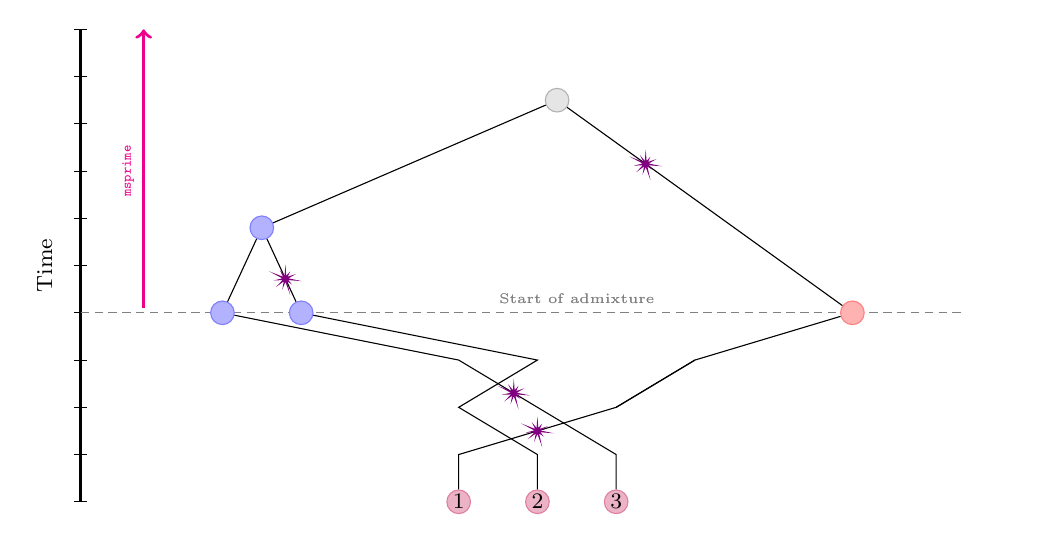
\begin{tikzpicture}[node distance=2mm and 2mm,xscale=.8,yscale=.6,font=\tiny]

\tikzset{greynode/.style={font=\footnotesize,node distance=1cm and 1 cm,fill=black!10,draw=black!30,inner sep=0pt,minimum size=3mm,shape=circle},
rednode/.style={font=\footnotesize,node distance=1cm and 1 cm,fill=red!30,draw=red!50,inner sep=0pt,minimum size=3mm,shape=circle},
bluenode/.style={font=\footnotesize,node distance=1cm and 1 cm,fill=blue!30,draw=blue!50,inner sep=0pt,minimum size=3mm,shape=circle},
purplenode/.style={font=\footnotesize,node distance=1cm and 1cm,fill=purple!30,draw=purple!50,inner sep=0pt,minimum size=3mm,shape=circle},
whitenode/.style={font=\footnotesize,node distance=1cm and 1cm,fill=white,draw=white,inner sep=0pt,minimum size=3.3mm,shape=circle},
mutations/.style={shape=starburst,fill=red!50!blue,inner sep=0.8pt,starburst points=11,starburst point height=.2cm}}

% Axis
\node (leftAx) at (-6,0) {};
\draw[very thick] (-6,0) -- +(0, 10);
\foreach \y in {0, 1, 2, 3, 4, 5, 6, 7, 8, 9, 10} \draw ($(leftAx) + (-0.1, \y)$) -- ($(leftAx) + (0.1, \y)$); % tick marks
\node[rotate=90,anchor=south] (leftLabel) at ($(leftAx) + (-0.3,5)$) {$\footnotesize\textrm{Time}$};

% Important times
\draw[gray,densely dashed] ($(leftAx) + (0,4)$) -- +(14, 0);

% Sample nodes
\node[purplenode] (s1) at (0,0) {1};
\node (s2) [purplenode,right of=s1] {2};
\node (s3) [purplenode,right of=s2] {3};
\node (s4) [purplenode,right of=s3] {};
%
%% Other purple nodes
%
\foreach \x in {1,2,3,4} \foreach \y in {1,2,3} \node[purplenode] (u\x\y) at ($(s\x) + (0, \y)$) {};

% Ancestral nodes
\node (pop1) at (-5, 4) {};
\node (pop2) at (5, 4) {};
\foreach \x in {2,3} \node[bluenode] (b\x) at ($(pop1) + (s\x)$) {};
\foreach \x in {1,4} \node (b\x) at ($(pop1) + (s\x)$) {};
\foreach \x in {1,3,4} \node (r\x) at ($(pop2) + (s\x)$) {};
\node[rednode] (r2) at ($(pop2) + (s2)$) {};

% white nodes
\node[whitenode] at (u42){}; \node[whitenode] at (u33){};
\node[whitenode] at (s4){}; \node[whitenode] at (u41){};
\foreach \x in {1,2,3,4} \foreach \y in {1,2,3} \node[whitenode] (u\x\y) at ($(s\x) + (0, \y)$) {};

% samples
%\draw[red,very thick] ($(s1.north)+(-.3,.3)$) -- ($(s3.north) + (.3,.3)$) -- ($(s3.south) + (.3,-.3)$) -- ($(s1.south)+(-.3,-.3)$)-- cycle;

% Time of admixture
\node[anchor=south,color=gray] at ($0.5*(b4) + 0.5*(r1)$) {{\tiny Start of admixture}};

% SLiM-simulated edges
\draw (s1) -- (u11.center) -- (u32.center) -- (u43.center) -- (r2);
\draw (s2) -- (u21.center) -- (u12.center) -- (u23.center) -- (b3);
\draw (s3) -- (u31.center) -- (u22.center) -- (u13.center) -- (b2);
\draw (u32.center) -- (u43.center);

% msprime nodes
\node[bluenode] (b5) at ($0.5*(b2)+0.5*(b3)+(0,1.8)$) {}; 
\node[greynode] (g1) at ($0.5*(b5)+0.5*(r2)+(0,3.6)$) {};

% msprime edges
\draw (b2) -- (b5) -- (b3); \draw (b5) -- (g1) -- (r2);

% simulation label
\draw[very thick,->,magenta] ($(b1) + (0,0.1)$) -- +(0,5.9);
\node[rotate=90,anchor=south,magenta] (msprime) at ($(b1) + (0,3)$) {$\texttt{msprime}$};

% Time of admixture
\node[anchor=south,color=gray] at ($0.5*(b4) + 0.5*(r1)$) {{\tiny Start of admixture}};

% Mutations
\node[mutations] at ($(u11)!.5!(u32)$) {};
\node[mutations] at ($(u13)!.7!(u22)$) {};
\node[mutations] at ($(b5)!.6!(b3)$) {};
\node[mutations] at ($(r2)!.7!(g1)$) {};

\end{tikzpicture} 

\end{center}
\end{frame}

\begin{frame}
\frametitle{New method performance}
\begin{center}
\small
\centering
\setlength{\aboverulesep}{5pt}
\setlength{\belowrulesep}{5pt}
\begin{tabularx}{1\textwidth}{p{3.5cm}p{2cm}p{1.9cm}p{1.9cm}X}
\toprule
%& \multicolumn{3}{c}{{\bf Global ancestry}} \\[1mm]
 & Missing data & Run time &  File size & Realism \\
\midrule 
%{\bf \texttt{msprime}} & $4.0$\% & 6 sec & 9 Mb & \crossmark \\ \addlinespace
{\bf \texttt{msprime}}  & $0.0$\% & 53 sec & 1700 Mb  & \crossmark \\ \addlinespace
%{\bf + migration records} & $0.0$\% &  & & \crossmark \\ 
%\midrule
%{\bf \texttt{SLiM}} & $4.0$\% & 10 min & 16 Mb  & \checkmark \\ \addlinespace
{\bf \texttt{SLiM}}& {$0.0$\%} & $>1$ hr  &  41 Mb & {\checkmark} \\ \addlinespace
%\midrule
{\bf\magenta{Georgia}} & \magenta{$0.0$\%} & \magenta{86 sec} & \magenta{39 Mb}  & \magenta{\checkmark} \\ \addlinespace
\bottomrule
\end{tabularx}
\end{center}
\vspace{5mm}
\end{frame}


%\section{Q. Can these methods simulate local ancestry?}
%
%
%
%
%\begin{frame}
%\frametitle{\texttt{SLiM} results}
%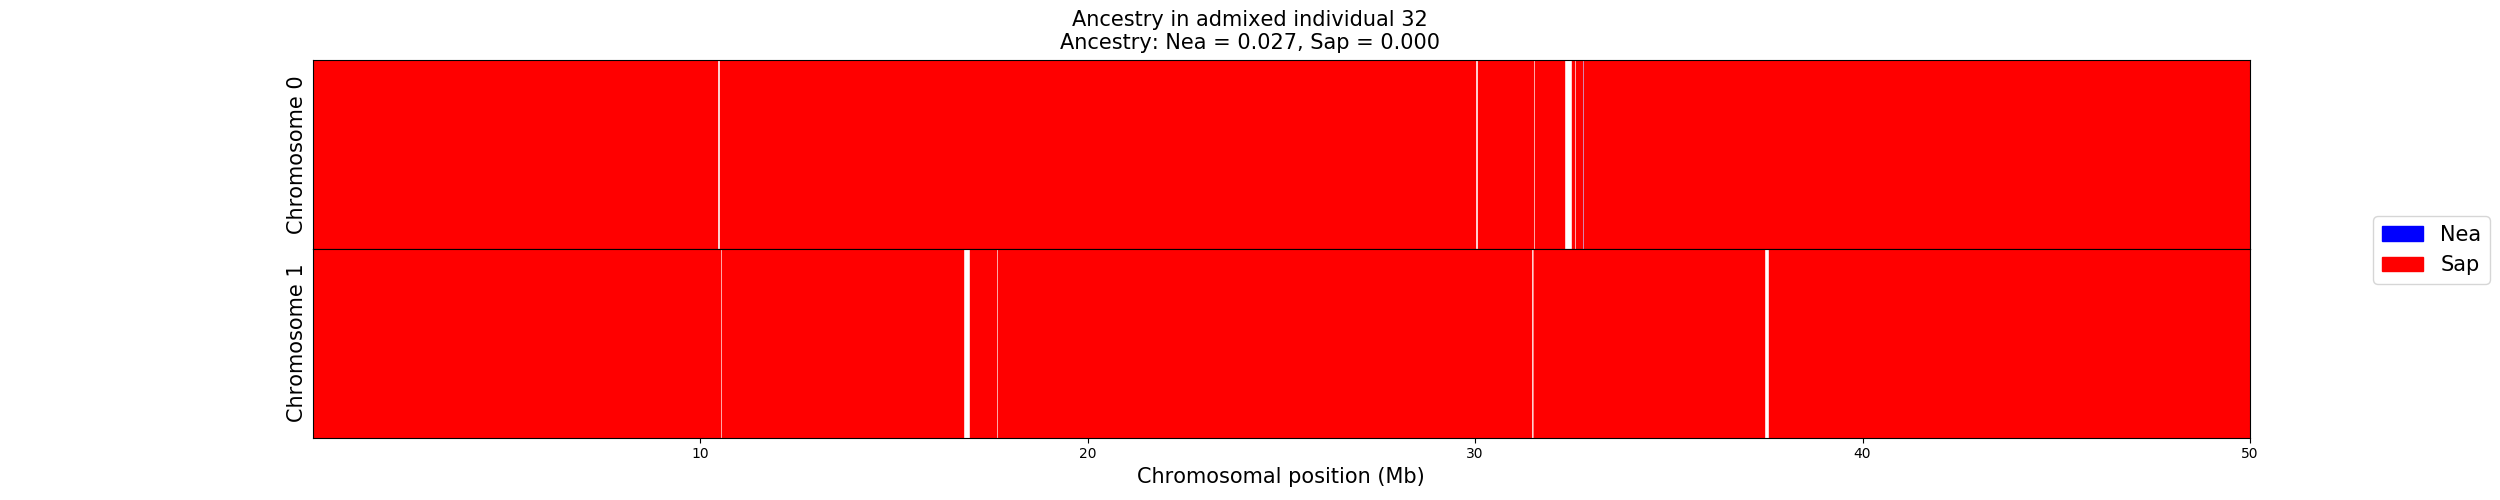
\includegraphics[scale=.22]{pics/slim-sample.png}\quad\quad
%Global ancestry averaged over all of the simulated samples was 
%\begin{itemize}
%\item $96.2\%$ Sapiens
%\item $<0.05\%$ Neanderthal
%\item \magenta{$3.8\%$ unassigned.}
%\end{itemize}
%%0.960 Sapiens, 0.000 Neanderthal, \magenta{0.040 unassigned.}
%\end{frame}
%
%\begin{frame}
%\frametitle{\texttt{SLiM} results - missing ancestry}
%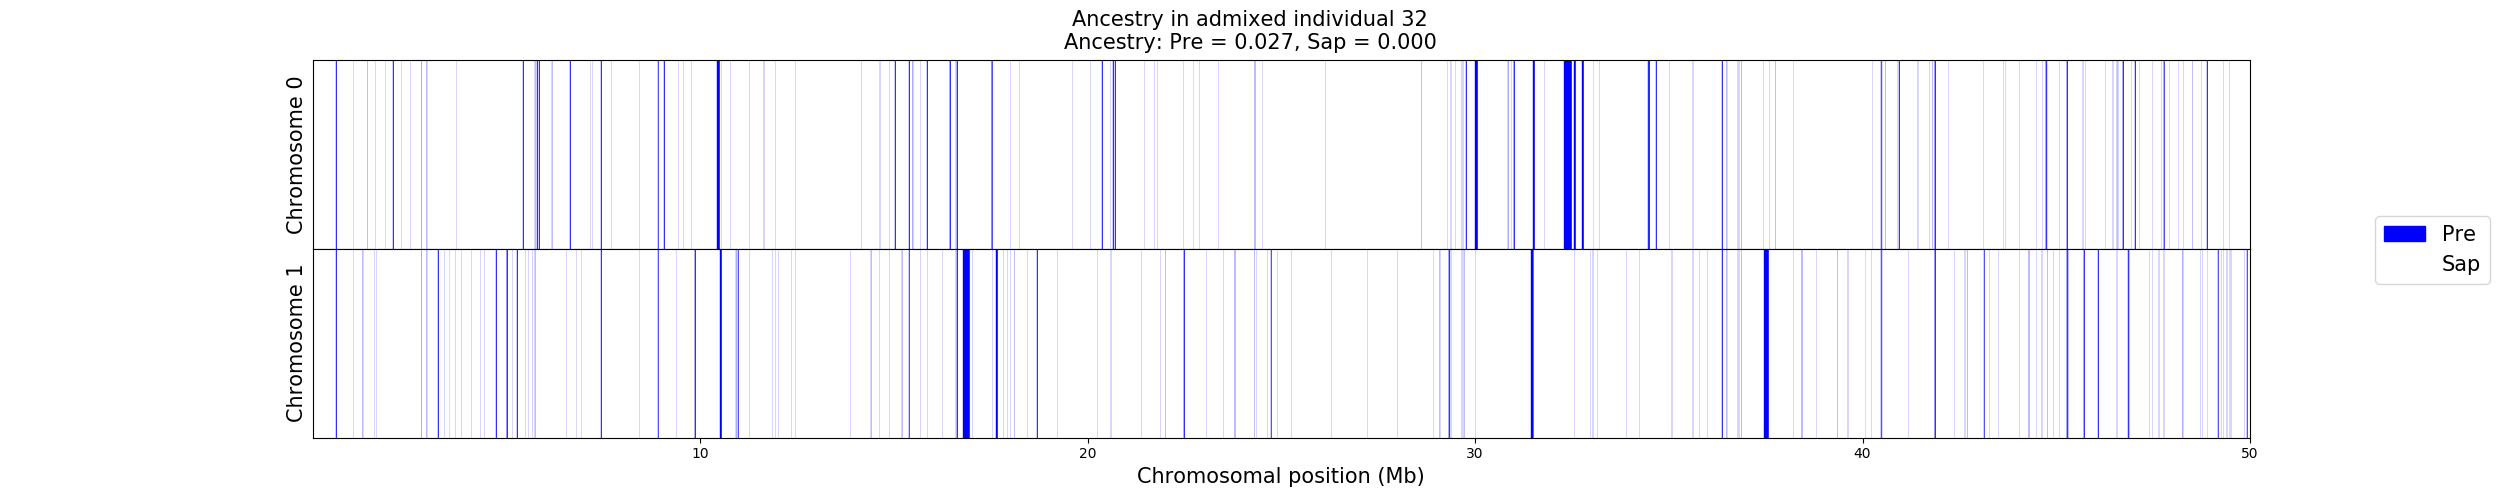
\includegraphics[scale=.22]{pics/slim-sample-missing.png}\quad\quad
%Global ancestry averaged over all of the simulated samples was 
%\begin{itemize}
%\item $96.2\%$ Sapiens
%\item $<0.05\%$ Neanderthal
%\item \magenta{$3.8\%$ unassigned.}
%\end{itemize}
%%0.960 Sapiens, 0.000 Neanderthal, \magenta{0.040 unassigned.}
%\end{frame}
%
%
%
%%\section{A new method for simulating admixture}
%%
%%\begin{frame}
%%\begin{center}
%%\centering
%%
\begin{tikzpicture}[node distance=2mm and 2mm,xscale=.8,yscale=.6,font=\tiny]

\tikzset{greynode/.style={font=\footnotesize,node distance=1cm and 1 cm,fill=black!10,draw=black!30,inner sep=0pt,minimum size=3mm,shape=circle},
rednode/.style={font=\footnotesize,node distance=1cm and 1 cm,fill=red!30,draw=red!50,inner sep=0pt,minimum size=3mm,shape=circle},
bluenode/.style={font=\footnotesize,node distance=1cm and 1 cm,fill=blue!30,draw=blue!50,inner sep=0pt,minimum size=3mm,shape=circle},
purplenode/.style={font=\footnotesize,node distance=1cm and 1cm,fill=purple!30,draw=purple!50,inner sep=0pt,minimum size=3mm,shape=circle},
whitenode/.style={font=\footnotesize,node distance=1cm and 1cm,fill=white,draw=white,inner sep=0pt,minimum size=3.3mm,shape=circle}}

% Axis
\node (leftAx) at (-6,0) {};
\draw[very thick] (-6,0) -- +(0, 10);
\foreach \y in {0, 1, 2, 3, 4, 5, 6, 7, 8, 9, 10} \draw ($(leftAx) + (-0.1, \y)$) -- ($(leftAx) + (0.1, \y)$); % tick marks
\node[rotate=90,anchor=south] (leftLabel) at ($(leftAx) + (-0.3,5)$) {$\footnotesize\textrm{Time}$};

% Important times
\draw[gray,densely dashed] ($(leftAx) + (0,4)$) -- +(16, 0);

% Sample nodes
\node(s1) [purplenode] at (0,0) {};
\node (s2) [purplenode,right of=s1] {};
\node (s3) [purplenode,right of=s2] {};
\node (s4) [purplenode,right of=s3] {};
%
%% Other purple nodes
%
%\foreach \x in {1,2,3,4} \foreach \y in {1,2,3} \node[purplenode] (u\x\y) at ($(s\x) + (0, \y)$) {};

% Ancestral nodes
\node (pop1) at (-5, 4) {};
\node (pop2) at (5, 4) {};
\foreach \x in {1,2,3,4} \node[bluenode] (b\x) at ($(pop1) + (s\x)$) {};
\foreach \x in {1,2,3,4} \node[rednode] (r\x) at ($(pop2) + (s\x)$) {};

% SLiM-simulated edges
%\draw (s1) -- (u11) -- (u32) -- (u43) -- (r2);
%\draw (s2) -- (u21) -- (u12) -- (u23) -- (b3);
%\draw (s3) -- (u31) -- (u22) -- (u13) -- (b2);
%\draw (s4) -- (u41) -- (u32) -- (u43);
%\draw (u42) -- (u33) -- (r1);

% Population labels
\node at ($0.5*(s2) + 0.5*(s3) + (0,-0.5)$) {$\tiny\textrm{Admixed population}$};
\node at ($(pop1) + 0.5*(s2) + 0.5*(s3) + (0,+0.5)$) {$\tiny\textrm{Blue ancestors}$};
\node at ($(pop2) + 0.5*(s2) + 0.5*(s3) + (0,+0.5)$) {$\tiny\textrm{Red ancestors}$};

% Cover the bottom bit
\foreach \x in {1,2,3,4} \node[whitenode] at (s\x) {};

% Time of admixture
\node[anchor=south,color=gray] at ($0.5*(b4) + 0.5*(r1)$) {{\tiny Start of admixture}};

\end{tikzpicture} 

%%\end{center}
%%\end{frame}
%%
%%\begin{frame}
%%\begin{center}
%%\centering
%%
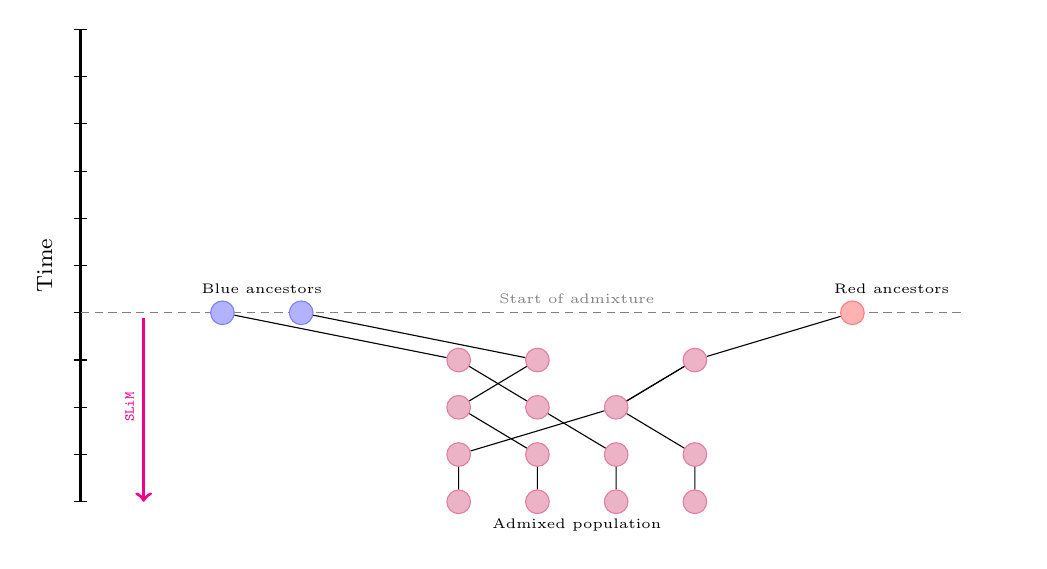
\begin{tikzpicture}[node distance=2mm and 2mm,xscale=.8,yscale=.6,font=\tiny]

\tikzset{greynode/.style={font=\footnotesize,node distance=1cm and 1 cm,fill=black!10,draw=black!30,inner sep=0pt,minimum size=3mm,shape=circle},
rednode/.style={font=\footnotesize,node distance=1cm and 1 cm,fill=red!30,draw=red!50,inner sep=0pt,minimum size=3mm,shape=circle},
bluenode/.style={font=\footnotesize,node distance=1cm and 1 cm,fill=blue!30,draw=blue!50,inner sep=0pt,minimum size=3mm,shape=circle},
purplenode/.style={font=\footnotesize,node distance=1cm and 1cm,fill=purple!30,draw=purple!50,inner sep=0pt,minimum size=3mm,shape=circle},
whitenode/.style={font=\footnotesize,node distance=1cm and 1cm,fill=white,draw=white,inner sep=0pt,minimum size=3.3mm,shape=circle}}

% Axis
\node (leftAx) at (-6,0) {};
\draw[very thick] (-6,0) -- +(0, 10);
\foreach \y in {0, 1, 2, 3, 4, 5, 6, 7, 8, 9, 10} \draw ($(leftAx) + (-0.1, \y)$) -- ($(leftAx) + (0.1, \y)$); % tick marks
\node[rotate=90,anchor=south] (leftLabel) at ($(leftAx) + (-0.3,5)$) {\footnotesize$\textrm{Time}$};

% Important times
\draw[gray,densely dashed] ($(leftAx) + (0,4)$) -- +(14, 0);

% Sample nodes
\node[purplenode] (s1) at (0,0) {};
\node (s2) [purplenode,right of=s1] {};
\node (s3) [purplenode,right of=s2] {};
\node (s4) [purplenode,right of=s3] {};
%
%% Other purple nodes
%
\foreach \x in {1,2,3,4} \foreach \y in {1,2,3} \node[purplenode] (u\x\y) at ($(s\x) + (0, \y)$) {};

% Ancestral nodes
\node (pop1) at (-5, 4) {};
\node (pop2) at (5, 4) {};
\foreach \x in {2,3} \node[bluenode] (b\x) at ($(pop1) + (s\x)$) {};
\foreach \x in {1,4} \node (b\x) at ($(pop1) + (s\x)$) {};
\foreach \x in {1,3,4} \node (r\x) at ($(pop2) + (s\x)$) {};
\node[rednode] (r2) at ($(pop2) + (s2)$) {};

% SLiM-simulated edges
\draw (s1) -- (u11) -- (u32) -- (u43) -- (r2);
\draw (s2) -- (u21) -- (u12) -- (u23) -- (b3);
\draw (s3) -- (u31) -- (u22) -- (u13) -- (b2);
\draw (s4) -- (u41) -- (u32) -- (u43);

% Population labels
\node at ($0.5*(s2) + 0.5*(s3) + (0,-0.5)$) {$\tiny\textrm{Admixed population}$};
\node at ($(pop1) + 0.5*(s2) + 0.5*(s3) + (0,+0.5)$) {$\tiny\textrm{Blue ancestors}$};
\node at ($(pop2) + 0.5*(s2) + 0.5*(s3) + (0,+0.5)$) {$\tiny\textrm{Red ancestors}$};

% white nodes
\node[whitenode] at (u42){}; \node[whitenode] at (u33){};

% simulation label
\draw[very thick,<-,magenta] ($(s1) + (-5,0)$) -- +(0,3.9);
\node[rotate=90,anchor=south,magenta] (SLiM) at ($(s1) + (-5,0) + (0,2)$) {$\texttt{SLiM}$};

% Time of admixture
\node[anchor=south,color=gray] at ($0.5*(b4) + 0.5*(r1)$) {{\tiny Start of admixture}};

\end{tikzpicture} 

%%\end{center}
%%\end{frame}
%%
%%\begin{frame}
%%\begin{center}
%%\centering
%%
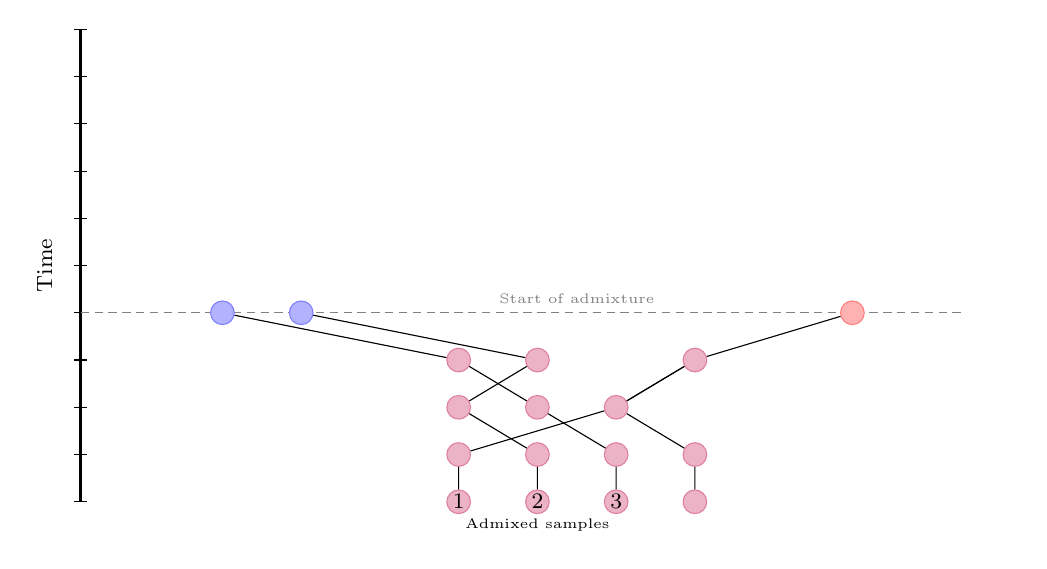
\begin{tikzpicture}[node distance=2mm and 2mm,xscale=.8,yscale=.6,font=\tiny]

\tikzset{greynode/.style={font=\footnotesize,node distance=1cm and 1 cm,fill=black!10,draw=black!30,inner sep=0pt,minimum size=3mm,shape=circle},
rednode/.style={font=\footnotesize,node distance=1cm and 1 cm,fill=red!30,draw=red!50,inner sep=0pt,minimum size=3mm,shape=circle},
bluenode/.style={font=\footnotesize,node distance=1cm and 1 cm,fill=blue!30,draw=blue!50,inner sep=0pt,minimum size=3mm,shape=circle},
purplenode/.style={font=\footnotesize,node distance=1cm and 1cm,fill=purple!30,draw=purple!50,inner sep=0pt,minimum size=3mm,shape=circle},
whitenode/.style={font=\footnotesize,node distance=1cm and 1cm,fill=white,draw=white,inner sep=0pt,minimum size=3.3mm,shape=circle}}

% Axis
\node (leftAx) at (-6,0) {};
\draw[very thick] (-6,0) -- +(0, 10);
\foreach \y in {0, 1, 2, 3, 4, 5, 6, 7, 8, 9, 10} \draw ($(leftAx) + (-0.1, \y)$) -- ($(leftAx) + (0.1, \y)$); % tick marks
\node[rotate=90,anchor=south] (leftLabel) at ($(leftAx) + (-0.3,5)$) {\footnotesize$\textrm{Time}$};

% Important times
\draw[gray,densely dashed] ($(leftAx) + (0,4)$) -- +(14, 0);

% Sample nodes
\node[purplenode] (s1) at (0,0) {1};
\node (s2) [purplenode,right of=s1] {2};
\node (s3) [purplenode,right of=s2] {3};
\node (s4) [purplenode,right of=s3] {};
%
%% Other purple nodes
%
\foreach \x in {1,2,3,4} \foreach \y in {1,2,3} \node[purplenode] (u\x\y) at ($(s\x) + (0, \y)$) {};

% Ancestral nodes
\node (pop1) at (-5, 4) {};
\node (pop2) at (5, 4) {};
\foreach \x in {2,3} \node[bluenode] (b\x) at ($(pop1) + (s\x)$) {};
\foreach \x in {1,4} \node (b\x) at ($(pop1) + (s\x)$) {};
\foreach \x in {1,3,4} \node (r\x) at ($(pop2) + (s\x)$) {};
\node[rednode] (r2) at ($(pop2) + (s2)$) {};

% SLiM-simulated edges
\draw (s1) -- (u11) -- (u32) -- (u43) -- (r2);
\draw (s2) -- (u21) -- (u12) -- (u23) -- (b3);
\draw (s3) -- (u31) -- (u22) -- (u13) -- (b2);
\draw (s4) -- (u41) -- (u32) -- (u43);

% Population labels
%\node at ($0.5*(s1) + 0.5*(s3) + (0,-0.5)$) {$\tiny\textrm{Admixed samples}$};

% white nodes
\node[whitenode] at (u42){}; \node[whitenode] at (u33){};

% samples
%\draw[red,very thick] ($(s1.north)+(-.3,.3)$) -- ($(s3.north) + (.3,.3)$) -- ($(s3.south) + (.3,-.3)$) -- ($(s1.south)+(-.3,-.3)$)-- cycle;

% Time of admixture
\node[anchor=south,color=gray] at ($0.5*(b4) + 0.5*(r1)$) {{\tiny Start of admixture}};

% Population labels
\node at ($0.5*(s1) + 0.5*(s3) + (0,-0.5)$) {$\tiny\textrm{Admixed samples}$};

\end{tikzpicture} 

%%\end{center}
%%\end{frame}
%%
%%\begin{frame}
%%\begin{center}
%%\centering
%%
\begin{tikzpicture}[node distance=2mm and 2mm,xscale=.8,yscale=.6,font=\tiny]

\tikzset{greynode/.style={font=\footnotesize,node distance=1cm and 1 cm,fill=black!10,draw=black!30,inner sep=0pt,minimum size=3mm,shape=circle},
rednode/.style={font=\footnotesize,node distance=1cm and 1 cm,fill=red!30,draw=red!50,inner sep=0pt,minimum size=3mm,shape=circle},
bluenode/.style={font=\footnotesize,node distance=1cm and 1 cm,fill=blue!30,draw=blue!50,inner sep=0pt,minimum size=3mm,shape=circle},
purplenode/.style={font=\footnotesize,node distance=1cm and 1cm,fill=purple!30,draw=purple!50,inner sep=0pt,minimum size=3mm,shape=circle},
whitenode/.style={font=\footnotesize,node distance=1cm and 1cm,fill=white,draw=white,inner sep=0pt,minimum size=3.3mm,shape=circle}}

% Axis
\node (leftAx) at (-6,0) {};
\draw[very thick] (-6,0) -- +(0, 10);
\foreach \y in {0, 1, 2, 3, 4, 5, 6, 7, 8, 9, 10} \draw ($(leftAx) + (-0.1, \y)$) -- ($(leftAx) + (0.1, \y)$); % tick marks
\node[rotate=90,anchor=south] (leftLabel) at ($(leftAx) + (-0.3,5)$) {$\footnotesize\textrm{Time}$};

% Important times
\draw[gray,densely dashed] ($(leftAx) + (0,4)$) -- +(14, 0);

% Sample nodes
\node[purplenode] (s1) at (0,0) {1};
\node (s2) [purplenode,right of=s1] {2};
\node (s3) [purplenode,right of=s2] {3};
\node (s4) [purplenode,right of=s3] {};
%
%% Other purple nodes
%
\foreach \x in {1,2,3,4} \foreach \y in {1,2,3} \node[purplenode] (u\x\y) at ($(s\x) + (0, \y)$) {};

% Ancestral nodes
\node (pop1) at (-5, 4) {};
\node (pop2) at (5, 4) {};
\foreach \x in {2,3} \node[bluenode] (b\x) at ($(pop1) + (s\x)$) {};
\foreach \x in {1,4} \node (b\x) at ($(pop1) + (s\x)$) {};
\foreach \x in {1,3,4} \node (r\x) at ($(pop2) + (s\x)$) {};
\node[rednode] (r2) at ($(pop2) + (s2)$) {};

% Population labels
\node at ($0.5*(s1) + 0.5*(s3) + (0,-0.5)$) {$\tiny\textrm{Admixed samples}$};

% Population labels
%\node at ($0.5*(s1) + 0.5*(s3) + (0,-0.5)$) {$\tiny\textrm{Admixed samples}$};

% white nodes
\node[whitenode] at (u42){}; \node[whitenode] at (u33){};
\node[whitenode] at (s4){}; \node[whitenode] at (u41){};
\foreach \x in {1,2,3,4} \foreach \y in {1,2,3} \node[whitenode] (u\x\y) at ($(s\x) + (0, \y)$) {};

% samples
%\draw[red,very thick] ($(s1.north)+(-.3,.3)$) -- ($(s3.north) + (.3,.3)$) -- ($(s3.south) + (.3,-.3)$) -- ($(s1.south)+(-.3,-.3)$)-- cycle;

% Time of admixture
\node[anchor=south,color=gray] at ($0.5*(b4) + 0.5*(r1)$) {{\tiny Start of admixture}};

% SLiM-simulated edges
\draw (s1) -- (u11.center) -- (u32.center) -- (u43.center) -- (r2);
\draw (s2) -- (u21.center) -- (u12.center) -- (u23.center) -- (b3);
\draw (s3) -- (u31.center) -- (u22.center) -- (u13.center) -- (b2);
\draw (u32.center) -- (u43.center);

\end{tikzpicture} 

%%\end{center}
%%\end{frame}
%%
%%\begin{frame}
%%\begin{center}
%%\centering
%%
\begin{tikzpicture}[node distance=2mm and 2mm,xscale=.8,yscale=.6,font=\tiny]

\tikzset{greynode/.style={font=\footnotesize,node distance=1cm and 1 cm,fill=black!10,draw=black!30,inner sep=0pt,minimum size=3mm,shape=circle},
rednode/.style={font=\footnotesize,node distance=1cm and 1 cm,fill=red!30,draw=red!50,inner sep=0pt,minimum size=3mm,shape=circle},
bluenode/.style={font=\footnotesize,node distance=1cm and 1 cm,fill=blue!30,draw=blue!50,inner sep=0pt,minimum size=3mm,shape=circle},
purplenode/.style={font=\footnotesize,node distance=1cm and 1cm,fill=purple!30,draw=purple!50,inner sep=0pt,minimum size=3mm,shape=circle},
whitenode/.style={font=\footnotesize,node distance=1cm and 1cm,fill=white,draw=white,inner sep=0pt,minimum size=3.3mm,shape=circle},
mutations/.style={shape=starburst,fill=red!50!blue,inner sep=0.8pt,starburst points=11,starburst point height=.2cm}}

% Axis
\node (leftAx) at (-6,0) {};
\draw[very thick] (-6,0) -- +(0, 10);
\foreach \y in {0, 1, 2, 3, 4, 5, 6, 7, 8, 9, 10} \draw ($(leftAx) + (-0.1, \y)$) -- ($(leftAx) + (0.1, \y)$); % tick marks
\node[rotate=90,anchor=south] (leftLabel) at ($(leftAx) + (-0.3,5)$) {$\footnotesize\textrm{Time}$};

% Important times
\draw[gray,densely dashed] ($(leftAx) + (0,4)$) -- +(14, 0);

% Sample nodes
\node[purplenode] (s1) at (0,0) {1};
\node (s2) [purplenode,right of=s1] {2};
\node (s3) [purplenode,right of=s2] {3};
\node (s4) [purplenode,right of=s3] {};
%
%% Other purple nodes
%
\foreach \x in {1,2,3,4} \foreach \y in {1,2,3} \node[purplenode] (u\x\y) at ($(s\x) + (0, \y)$) {};

% Ancestral nodes
\node (pop1) at (-5, 4) {};
\node (pop2) at (5, 4) {};
\foreach \x in {2,3} \node[bluenode] (b\x) at ($(pop1) + (s\x)$) {};
\foreach \x in {1,4} \node (b\x) at ($(pop1) + (s\x)$) {};
\foreach \x in {1,3,4} \node (r\x) at ($(pop2) + (s\x)$) {};
\node[rednode] (r2) at ($(pop2) + (s2)$) {};

% Population labels
\node at ($0.5*(s1) + 0.5*(s3) + (0,-0.5)$) {$\tiny\textrm{Admixed samples}$};

% Population labels
%\node at ($0.5*(s1) + 0.5*(s3) + (0,-0.5)$) {$\tiny\textrm{Admixed samples}$};

% white nodes
\node[whitenode] at (u42){}; \node[whitenode] at (u33){};
\node[whitenode] at (s4){}; \node[whitenode] at (u41){};
\foreach \x in {1,2,3,4} \foreach \y in {1,2,3} \node[whitenode] (u\x\y) at ($(s\x) + (0, \y)$) {};

% samples
%\draw[red,very thick] ($(s1.north)+(-.3,.3)$) -- ($(s3.north) + (.3,.3)$) -- ($(s3.south) + (.3,-.3)$) -- ($(s1.south)+(-.3,-.3)$)-- cycle;

% Time of admixture
\node[anchor=south,color=gray] at ($0.5*(b4) + 0.5*(r1)$) {{\tiny Start of admixture}};

% SLiM-simulated edges
\draw (s1) -- (u11.center) -- (u32.center) -- (u43.center) -- (r2);
\draw (s2) -- (u21.center) -- (u12.center) -- (u23.center) -- (b3);
\draw (s3) -- (u31.center) -- (u22.center) -- (u13.center) -- (b2);
\draw (u32.center) -- (u43.center);

% Mutations
\node[mutations] at ($(u11)!.5!(u32)$) {};
\node[mutations] at ($(u13)!.7!(u22)$) {};

\end{tikzpicture} 

%%\end{center}
%%\end{frame}
%%
%%\begin{frame}
%%\begin{center}
%%\centering
%%
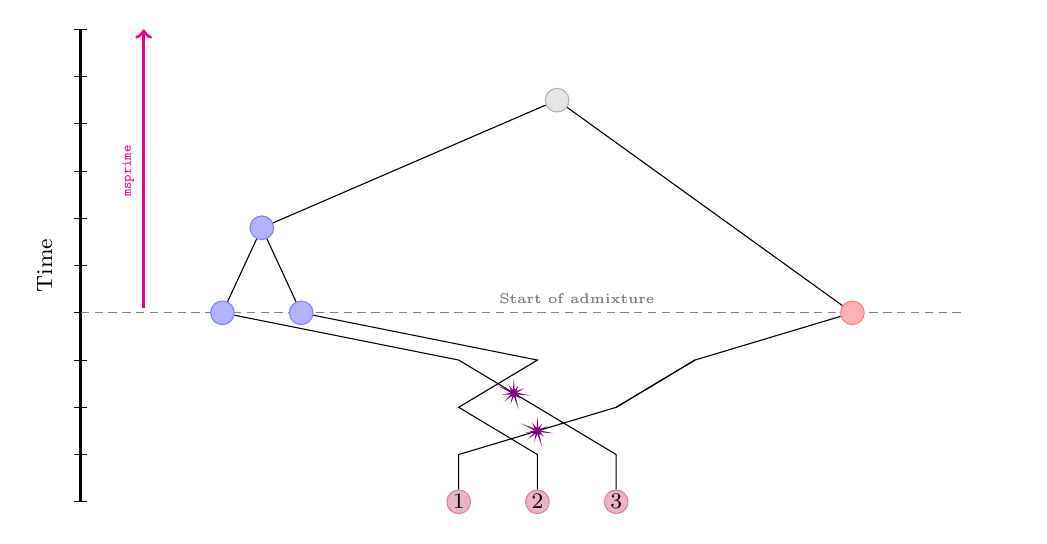
\begin{tikzpicture}[node distance=2mm and 2mm,xscale=.8,yscale=.6,font=\tiny]

\tikzset{greynode/.style={font=\footnotesize,node distance=1cm and 1 cm,fill=black!10,draw=black!30,inner sep=0pt,minimum size=3mm,shape=circle},
rednode/.style={font=\footnotesize,node distance=1cm and 1 cm,fill=red!30,draw=red!50,inner sep=0pt,minimum size=3mm,shape=circle},
bluenode/.style={font=\footnotesize,node distance=1cm and 1 cm,fill=blue!30,draw=blue!50,inner sep=0pt,minimum size=3mm,shape=circle},
purplenode/.style={font=\footnotesize,node distance=1cm and 1cm,fill=purple!30,draw=purple!50,inner sep=0pt,minimum size=3mm,shape=circle},
whitenode/.style={font=\footnotesize,node distance=1cm and 1cm,fill=white,draw=white,inner sep=0pt,minimum size=3.3mm,shape=circle},
mutations/.style={shape=starburst,fill=red!50!blue,inner sep=0.8pt,starburst points=11,starburst point height=.2cm}}

% Axis
\node (leftAx) at (-6,0) {};
\draw[very thick] (-6,0) -- +(0, 10);
\foreach \y in {0, 1, 2, 3, 4, 5, 6, 7, 8, 9, 10} \draw ($(leftAx) + (-0.1, \y)$) -- ($(leftAx) + (0.1, \y)$); % tick marks
\node[rotate=90,anchor=south] (leftLabel) at ($(leftAx) + (-0.3,5)$) {$\footnotesize\textrm{Time}$};

% Important times
\draw[gray,densely dashed] ($(leftAx) + (0,4)$) -- +(14, 0);

% Sample nodes
\node[purplenode] (s1) at (0,0) {1};
\node (s2) [purplenode,right of=s1] {2};
\node (s3) [purplenode,right of=s2] {3};
\node (s4) [purplenode,right of=s3] {};
%
%% Other purple nodes
%
\foreach \x in {1,2,3,4} \foreach \y in {1,2,3} \node[purplenode] (u\x\y) at ($(s\x) + (0, \y)$) {};

% Ancestral nodes
\node (pop1) at (-5, 4) {};
\node (pop2) at (5, 4) {};
\foreach \x in {2,3} \node[bluenode] (b\x) at ($(pop1) + (s\x)$) {};
\foreach \x in {1,4} \node (b\x) at ($(pop1) + (s\x)$) {};
\foreach \x in {1,3,4} \node (r\x) at ($(pop2) + (s\x)$) {};
\node[rednode] (r2) at ($(pop2) + (s2)$) {};

% white nodes
\node[whitenode] at (u42){}; \node[whitenode] at (u33){};
\node[whitenode] at (s4){}; \node[whitenode] at (u41){};
\foreach \x in {1,2,3,4} \foreach \y in {1,2,3} \node[whitenode] (u\x\y) at ($(s\x) + (0, \y)$) {};

% samples
%\draw[red,very thick] ($(s1.north)+(-.3,.3)$) -- ($(s3.north) + (.3,.3)$) -- ($(s3.south) + (.3,-.3)$) -- ($(s1.south)+(-.3,-.3)$)-- cycle;

% Time of admixture
\node[anchor=south,color=gray] at ($0.5*(b4) + 0.5*(r1)$) {{\tiny Start of admixture}};

% SLiM-simulated edges
\draw (s1) -- (u11.center) -- (u32.center) -- (u43.center) -- (r2);
\draw (s2) -- (u21.center) -- (u12.center) -- (u23.center) -- (b3);
\draw (s3) -- (u31.center) -- (u22.center) -- (u13.center) -- (b2);
\draw (u32.center) -- (u43.center);

% Mutations
\node[mutations] at ($(u11)!.5!(u32)$) {};
\node[mutations] at ($(u13)!.7!(u22)$) {};

% msprime nodes
\node[bluenode] (b5) at ($0.5*(b2)+0.5*(b3)+(0,1.8)$) {}; 
\node[greynode] (g1) at ($0.5*(b5)+0.5*(r2)+(0,3.6)$) {};

% msprime edges
\draw (b2) -- (b5) -- (b3); \draw (b5) -- (g1) -- (r2);

% simulation label
\draw[very thick,->,magenta] ($(b1) + (0,0.1)$) -- +(0,5.9);
\node[rotate=90,anchor=south,magenta] (msprime) at ($(b1) + (0,3)$) {$\texttt{msprime}$};

% Time of admixture
\node[anchor=south,color=gray] at ($0.5*(b4) + 0.5*(r1)$) {{\tiny Start of admixture}};

\end{tikzpicture} 

%%\end{center}
%%\end{frame}
%%
%%\begin{frame}
%%\begin{center}
%%\centering
%%
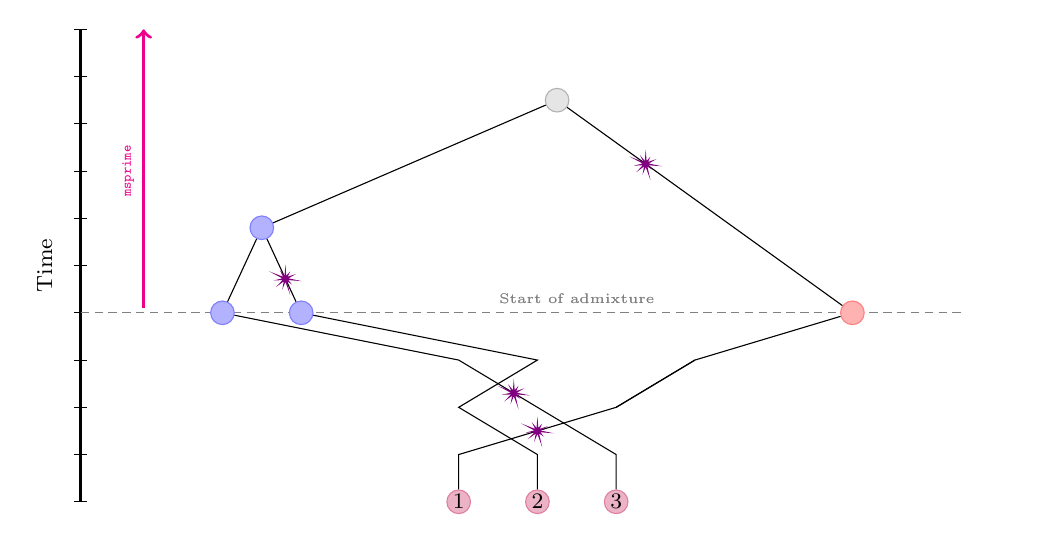
\begin{tikzpicture}[node distance=2mm and 2mm,xscale=.8,yscale=.6,font=\tiny]

\tikzset{greynode/.style={font=\footnotesize,node distance=1cm and 1 cm,fill=black!10,draw=black!30,inner sep=0pt,minimum size=3mm,shape=circle},
rednode/.style={font=\footnotesize,node distance=1cm and 1 cm,fill=red!30,draw=red!50,inner sep=0pt,minimum size=3mm,shape=circle},
bluenode/.style={font=\footnotesize,node distance=1cm and 1 cm,fill=blue!30,draw=blue!50,inner sep=0pt,minimum size=3mm,shape=circle},
purplenode/.style={font=\footnotesize,node distance=1cm and 1cm,fill=purple!30,draw=purple!50,inner sep=0pt,minimum size=3mm,shape=circle},
whitenode/.style={font=\footnotesize,node distance=1cm and 1cm,fill=white,draw=white,inner sep=0pt,minimum size=3.3mm,shape=circle},
mutations/.style={shape=starburst,fill=red!50!blue,inner sep=0.8pt,starburst points=11,starburst point height=.2cm}}

% Axis
\node (leftAx) at (-6,0) {};
\draw[very thick] (-6,0) -- +(0, 10);
\foreach \y in {0, 1, 2, 3, 4, 5, 6, 7, 8, 9, 10} \draw ($(leftAx) + (-0.1, \y)$) -- ($(leftAx) + (0.1, \y)$); % tick marks
\node[rotate=90,anchor=south] (leftLabel) at ($(leftAx) + (-0.3,5)$) {$\footnotesize\textrm{Time}$};

% Important times
\draw[gray,densely dashed] ($(leftAx) + (0,4)$) -- +(14, 0);

% Sample nodes
\node[purplenode] (s1) at (0,0) {1};
\node (s2) [purplenode,right of=s1] {2};
\node (s3) [purplenode,right of=s2] {3};
\node (s4) [purplenode,right of=s3] {};
%
%% Other purple nodes
%
\foreach \x in {1,2,3,4} \foreach \y in {1,2,3} \node[purplenode] (u\x\y) at ($(s\x) + (0, \y)$) {};

% Ancestral nodes
\node (pop1) at (-5, 4) {};
\node (pop2) at (5, 4) {};
\foreach \x in {2,3} \node[bluenode] (b\x) at ($(pop1) + (s\x)$) {};
\foreach \x in {1,4} \node (b\x) at ($(pop1) + (s\x)$) {};
\foreach \x in {1,3,4} \node (r\x) at ($(pop2) + (s\x)$) {};
\node[rednode] (r2) at ($(pop2) + (s2)$) {};

% white nodes
\node[whitenode] at (u42){}; \node[whitenode] at (u33){};
\node[whitenode] at (s4){}; \node[whitenode] at (u41){};
\foreach \x in {1,2,3,4} \foreach \y in {1,2,3} \node[whitenode] (u\x\y) at ($(s\x) + (0, \y)$) {};

% samples
%\draw[red,very thick] ($(s1.north)+(-.3,.3)$) -- ($(s3.north) + (.3,.3)$) -- ($(s3.south) + (.3,-.3)$) -- ($(s1.south)+(-.3,-.3)$)-- cycle;

% Time of admixture
\node[anchor=south,color=gray] at ($0.5*(b4) + 0.5*(r1)$) {{\tiny Start of admixture}};

% SLiM-simulated edges
\draw (s1) -- (u11.center) -- (u32.center) -- (u43.center) -- (r2);
\draw (s2) -- (u21.center) -- (u12.center) -- (u23.center) -- (b3);
\draw (s3) -- (u31.center) -- (u22.center) -- (u13.center) -- (b2);
\draw (u32.center) -- (u43.center);

% msprime nodes
\node[bluenode] (b5) at ($0.5*(b2)+0.5*(b3)+(0,1.8)$) {}; 
\node[greynode] (g1) at ($0.5*(b5)+0.5*(r2)+(0,3.6)$) {};

% msprime edges
\draw (b2) -- (b5) -- (b3); \draw (b5) -- (g1) -- (r2);

% simulation label
\draw[very thick,->,magenta] ($(b1) + (0,0.1)$) -- +(0,5.9);
\node[rotate=90,anchor=south,magenta] (msprime) at ($(b1) + (0,3)$) {$\texttt{msprime}$};

% Time of admixture
\node[anchor=south,color=gray] at ($0.5*(b4) + 0.5*(r1)$) {{\tiny Start of admixture}};

% Mutations
\node[mutations] at ($(u11)!.5!(u32)$) {};
\node[mutations] at ($(u13)!.7!(u22)$) {};
\node[mutations] at ($(b5)!.6!(b3)$) {};
\node[mutations] at ($(r2)!.7!(g1)$) {};

\end{tikzpicture} 

%%\end{center}
%%\end{frame}
%
%\begin{frame}
%\frametitle{Results}
%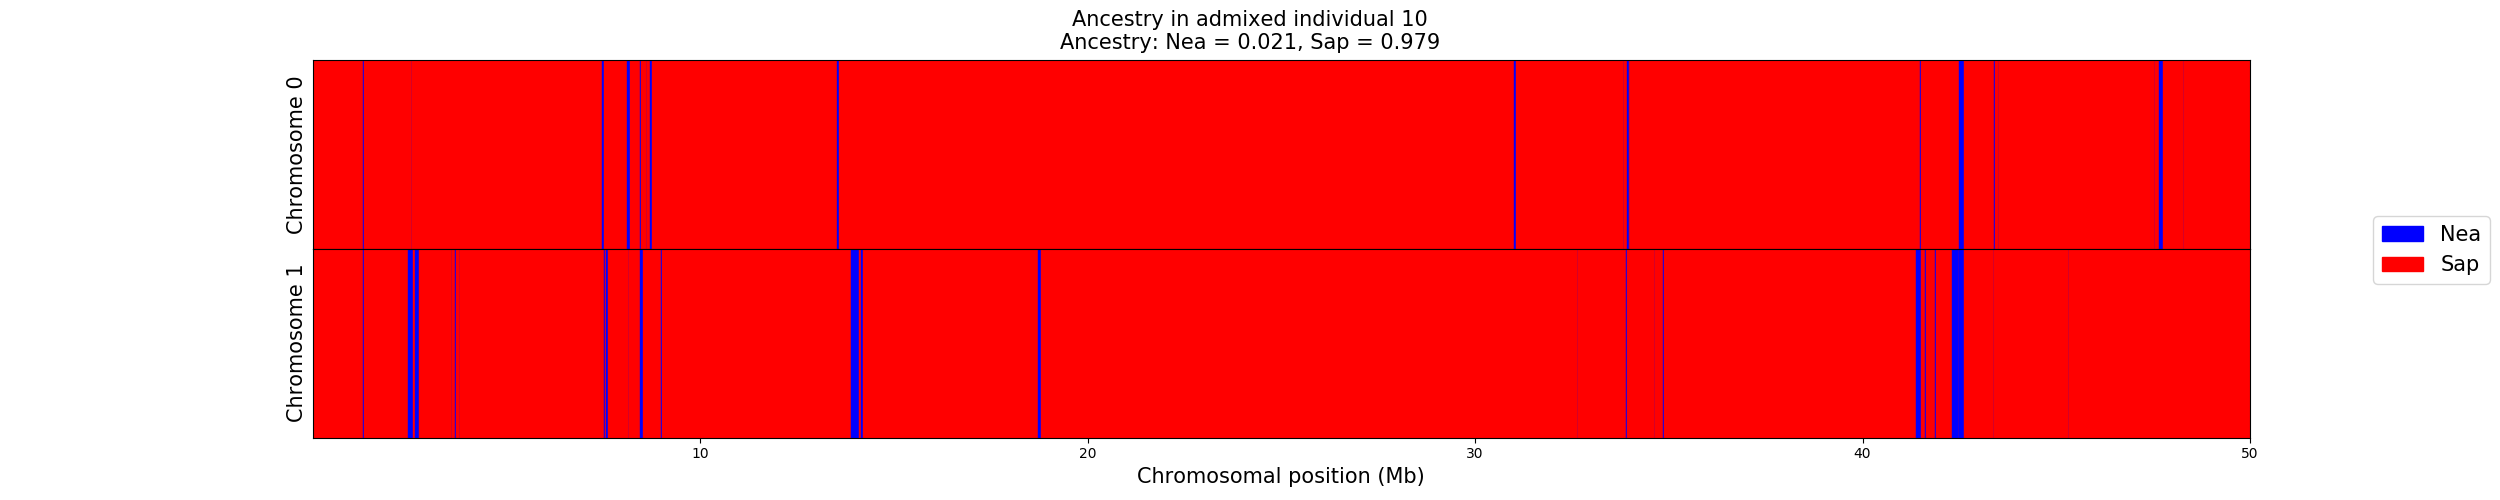
\includegraphics[scale=.22]{pics/new-method-sample.png}\quad\quad
%Global ancestry averaged over all of the simulated samples was 
%\begin{itemize}
%\item $98.0\%$ Sapiens
%\item $2.0\%$ Neanderthal
%\item \magenta{$0.0\%$ unassigned.}
%\end{itemize}
%%0.960 Sapiens, 0.000 Neanderthal, \magenta{0.040 unassigned.}
%\end{frame}
%
%\section{Why this work matters}
%
%\begin{frame}
%\begin{center}
%\small
%\centering
%\begin{tabularx}{.7\textwidth}{p{2.5cm}p{1.7cm}p{1.7cm}X}
%\toprule
%& \multicolumn{3}{c}{{\bf Global ancestry}} \\[1mm]
% & { Sapiens} & { Neanderthal} &  Missing \\
%\midrule 
%{\bf msprime} & $96.0$\% & $\approx 0.0$\% & $4.0\%$  \\[3mm]
%{\bf SLiM} & $96.2\%$ &  $\approx 0.0\%$ & $3.8\%$ \\[3mm]
%{\bf Georgia} & $98.0\%$ & $2.0\%$ & $0.0\%$  \\[3mm]
%\midrule
%{\bf\magenta{Expected}} & \magenta{$98.0\%$} & \magenta{$2.0\%$} & \magenta{$0.0\%$} \\[1mm]
%\bottomrule
%\end{tabularx}
%\end{center}
%\vspace{5mm}
%Affects the computation of ancestral tract lengths, population-specific frequency spectra, ancestry-informative markers...
%\end{frame}

%\begin{frame}
%\frametitle{Simulations are often used to benchmark methods\\ for inferring local ancestry}
%{\footnotesize
%Steinruecken, M., Spence, J. P., Kamm, J. A., Wieczorek, E., \& Song, Y. S. (2018). Model-based detection and analysis of introgressed Neanderthal ancestry in modern humans. \emph{Molecular Ecology, 27(19)}, pp. 3873 - 3888.
%}\\[2mm]
%
%\begin{center}
%\includegraphics[scale=.5]{pics/paper-2018Steinrucken/2018Steinrucken-1.png}\\[2mm]
%\includegraphics[scale=.5]{pics/paper-2018Steinrucken/2018Steinrucken-2.png}
%\end{center}
%\end{frame}
%
%\begin{frame}
%\frametitle{Testing your method on incomplete ancestral data\\
%makes it look better than it actually is}
%\begin{center}
%\includegraphics[scale=.5]{pics/paper-2018Steinrucken/2018Steinrucken-3.png}\\[10mm]
%\magenta{NOPE :(}
%\end{center}
%\end{frame}

%\begin{frame}
%\frametitle{Another example}
%{\small
%Browning, S. R., Browning, B. L., Zhou, Y., Tucci, S., \& Akey, J. M. (2018). Analysis of Human Sequence Data Reveals Two Pulses of Archaic Denisovan Admixture. \emph{Cell, 173(1),} 53–61
%}\\[2mm]
%\begin{center}
%\includegraphics[scale=.4]{pics/paper-2018Browning/2018Browning-1.png}\\[2mm]
%\includegraphics[scale=.4]{pics/paper-2018Browning/2018Browning-2.png}
%\end{center}
%This paper inferred a `true' introgression status of haplotypes simulated with msprime (?)
%
%\end{frame}

%\begin{frame}
%\frametitle{Ancestry inference methods trained on flawed simulations\\
%are likely to be biased
%}
%{\footnotesize
%Sankararaman, S. et al (2014). The genomic landscape of Neanderthal ancestry in present-day humans. \emph{Nature, 507(7492)}, pp. 354 - 357.
%}\\[2mm]
%\begin{center}
%\includegraphics[scale=.35]{pics/paper-2014Sankararaman/Sankararaman-1.png}\\[2mm]
%\includegraphics[scale=.4]{pics/paper-2014Sankararaman/Sankararaman-2.png}
%\end{center}
%\end{frame}

\begin{frame}
\frametitle{Summary}
\begin{wideitemize}
\item It is useful to keep track of local ancestry in genetic simulations.
\item Standard tree sequence simulators are able to do this with the help of efficient ancestry-extraction algorithms.
\item A new simulation method can do this quickly while also allowing the user to model complex admixture scenarios.
\end{wideitemize}
\end{frame}

\begin{frame}
\frametitle{Thanks to...}

\begin{tabularx}{.68\textwidth}{p{3cm}X}
My supervisors & $\begin{cases}
\mathrm{Damjan\ts\ts Vukcevic\ts\ts (University\ts\ts of\ts\ts Melbourne)} \\
\mathrm{Stephen\ts\ts Leslie\ts\ts (University\ts\ts of \ts\ts Melbourne)}
\end{cases}$\\ \addlinespace
My collaborators &
$\begin{cases}
\mathrm{Peter\ts\ts Ralph\ts\ts(University\ts\ts of\ts\ts Oregon)} \\
\mathrm{Jerome\ts\ts Kelleher\ts\ts(BDI,\ts\ts University\ts\ts of\ts\ts Oxford)}
\end{cases}$\\ \addlinespace
Sources of \$\ &
$\begin{cases}
\mathrm{Helen\ts\ts Freeman\ts\ts scholarship,\ts\ts UniMelb} \\
\mathrm{Maurice\ts\ts Belz\ts\ts Fund,\ts\ts UniMelb}\\
\mathrm{Research\ts\ts Training\ts\ts Scheme,\ts\ts Australian\ts\ts Government}
\end{cases}$\\ \addlinespace
\end{tabularx}

Special thanks to Jerome and the University of Oxford for hosting me in the UK this year.

%My supervisors\quad
\end{frame}

\begin{frame}
\frametitle{References}

{\bf \texttt{msprime} and tree sequences:}\\
Kelleher, J., et al. (2016). Efficient Coalescent Simulation and Genealogical Analysis for Large Sample Sizes. PLOS Computational Biology, 12(5).
\vspace{5mm}

{\bf \texttt{SLiM}:}\\
Galloway, J.,  et al. (2018). Tree-sequence recording in SLiM opens new horizons for forward-time simulation of whole genomes. Molecular Ecology Resources, (November 2018), 552–566.

\end{frame}

\end{document}